\documentclass{Fabiano_file}
\usepackage[table,usenames,dvipsnames]{xcolor}
\usepackage{tikz} %para desenhar
\usepackage{epstopdf}
\usepackage{hhline}
\usepackage{amsmath}
\usepackage{array}
\usepackage{cancel}
\usepackage{multirow}
\usepackage{bm}
\usepackage{float}
\usepackage{makecell} % diagonal table cells
\usepackage{tabularx}
\usepackage{bold-extra} % mini caps e negrito ao mesmo tempo %
\usepackage{fixltx2e} 
\usepackage{graphicx,amssymb}
\usepackage{subcaption} 
\usepackage{alltt}
\usepackage{mathtools}
\usepackage[figuresleft]{rotating}
\usepackage{caption}
\usepackage{varwidth}
\usepackage{longtable}

\usepackage[american,cuteinductors,smartlabels]{circuitikz}
\usepackage[hidelinks]{hyperref}
\usepackage[nottoc]{tocbibind}
\usepackage[a4paper,left=2cm,right=2cm,top=2cm,bottom=3cm]{geometry}

\usepackage{graphicx}
\usepackage{amssymb, amsmath, amsthm}
\usepackage{float}

\setcounter{secnumdepth}{5}

\usepackage{listings}
\usepackage{color}    %May be necessary if you want to color links
\usepackage{hyperref}
\hypersetup{
    colorlinks=true, %set true if you want colored links
    linktoc=all,     %set to all if you want both sections and subsections linked
    linkcolor=blue,  %choose some color if you want links to stand out
}
\lstset{language=C}


\title{Simulação do Microcontrolador 80c51 Utilizando o Software PROTEUS.\\Trabalho Baseado no Artigo:\\2010-Application of Proteus Virtual System Modelling (VSM) in Teaching of Microcontroller }
\author{Aluno: Fabiano Aparecido Marino \\NºUsp:7143980}

\begin{document}

	\newpage
	\thispagestyle{empty}
	\clearpage
	\begin{sidewaysfigure}
		\centering
		\includegraphics[width=1\linewidth]{capac_principal}
		\label{fig:capac_principal}
	\end{sidewaysfigure}
	\clearpage
	\pagenumbering{arabic}
	\newpage
	
\maketitle

\begin{figure}[h!]
\centering

\includegraphics[width=.9\textwidth]{capa.jpg}
\end{figure}

\newpage

\tableofcontents
\newpage

\listoffigures
\newpage

\section{Proteus}
O software proteus, oferecido pela empresa Labcenter Electronics, não é gratuito, apesar de haver a versao demo disponível no site da fabircante.
Possui diversos componentes tanto na área analógica quanto digital, estando muito deles disponíveis para simulação.
Em suas bibliotecas há componentes ideais, que fazem seu principio de funcionamento sem parametros de limitação, e componentes especificado por fabricantes, 
havendo também a possibilidade de se criar componentes, tanto em esquemático quanto em PCB (Printed Circuit Board) para fins de construção do esquemático 
produzido.Por enquanto o que se vê de diferencial é a presença de componentes digitais, e isso não se restringe a portas lógicas e flip-flops como 
encontra-se presente em diversos softwares de simulação, mas também com conversores AD e DA de vários fabricantes e micrcontroladores programáveis de 
diversos fabricantes, indo desde de ARM a outros menos robustos como a famosa família de controladores MCU8051.Display de sete segmentos e de cristal 
liquido também encontram-se presentes, permitindo a simulação  conjunta dos componentes citados.Memórias também encontram-se disponiveis para simulação 
e esquemático podendo ser usadas em simulação conjunta com outros periféricos.Concluindo, fica a critério do projetista como utilizar os vários componentes 
presentes no simulador.\\
Um outro fato que leva a utilização do proteus, é a relação que exite entre suas duas interface ISIS e ARES, que permite a construção do projeto esquemático
no ISIS posteriomente apenas transportando para o ARES com as ligações entre componentes já executada, oque é comum em softwares de PCB.
O que diferencia  o proteus é que o esquemático já possui sua simulação, assim o PCB só é executado quando o esquemático estiver funcionando, 
garantindo de primeira a construção do circuito.A figura (\ref{fig:Simulacao_proteus_esquematico_PCB}) ilustra essa vantagem.\\

\begin{figure}[h!]
\centering
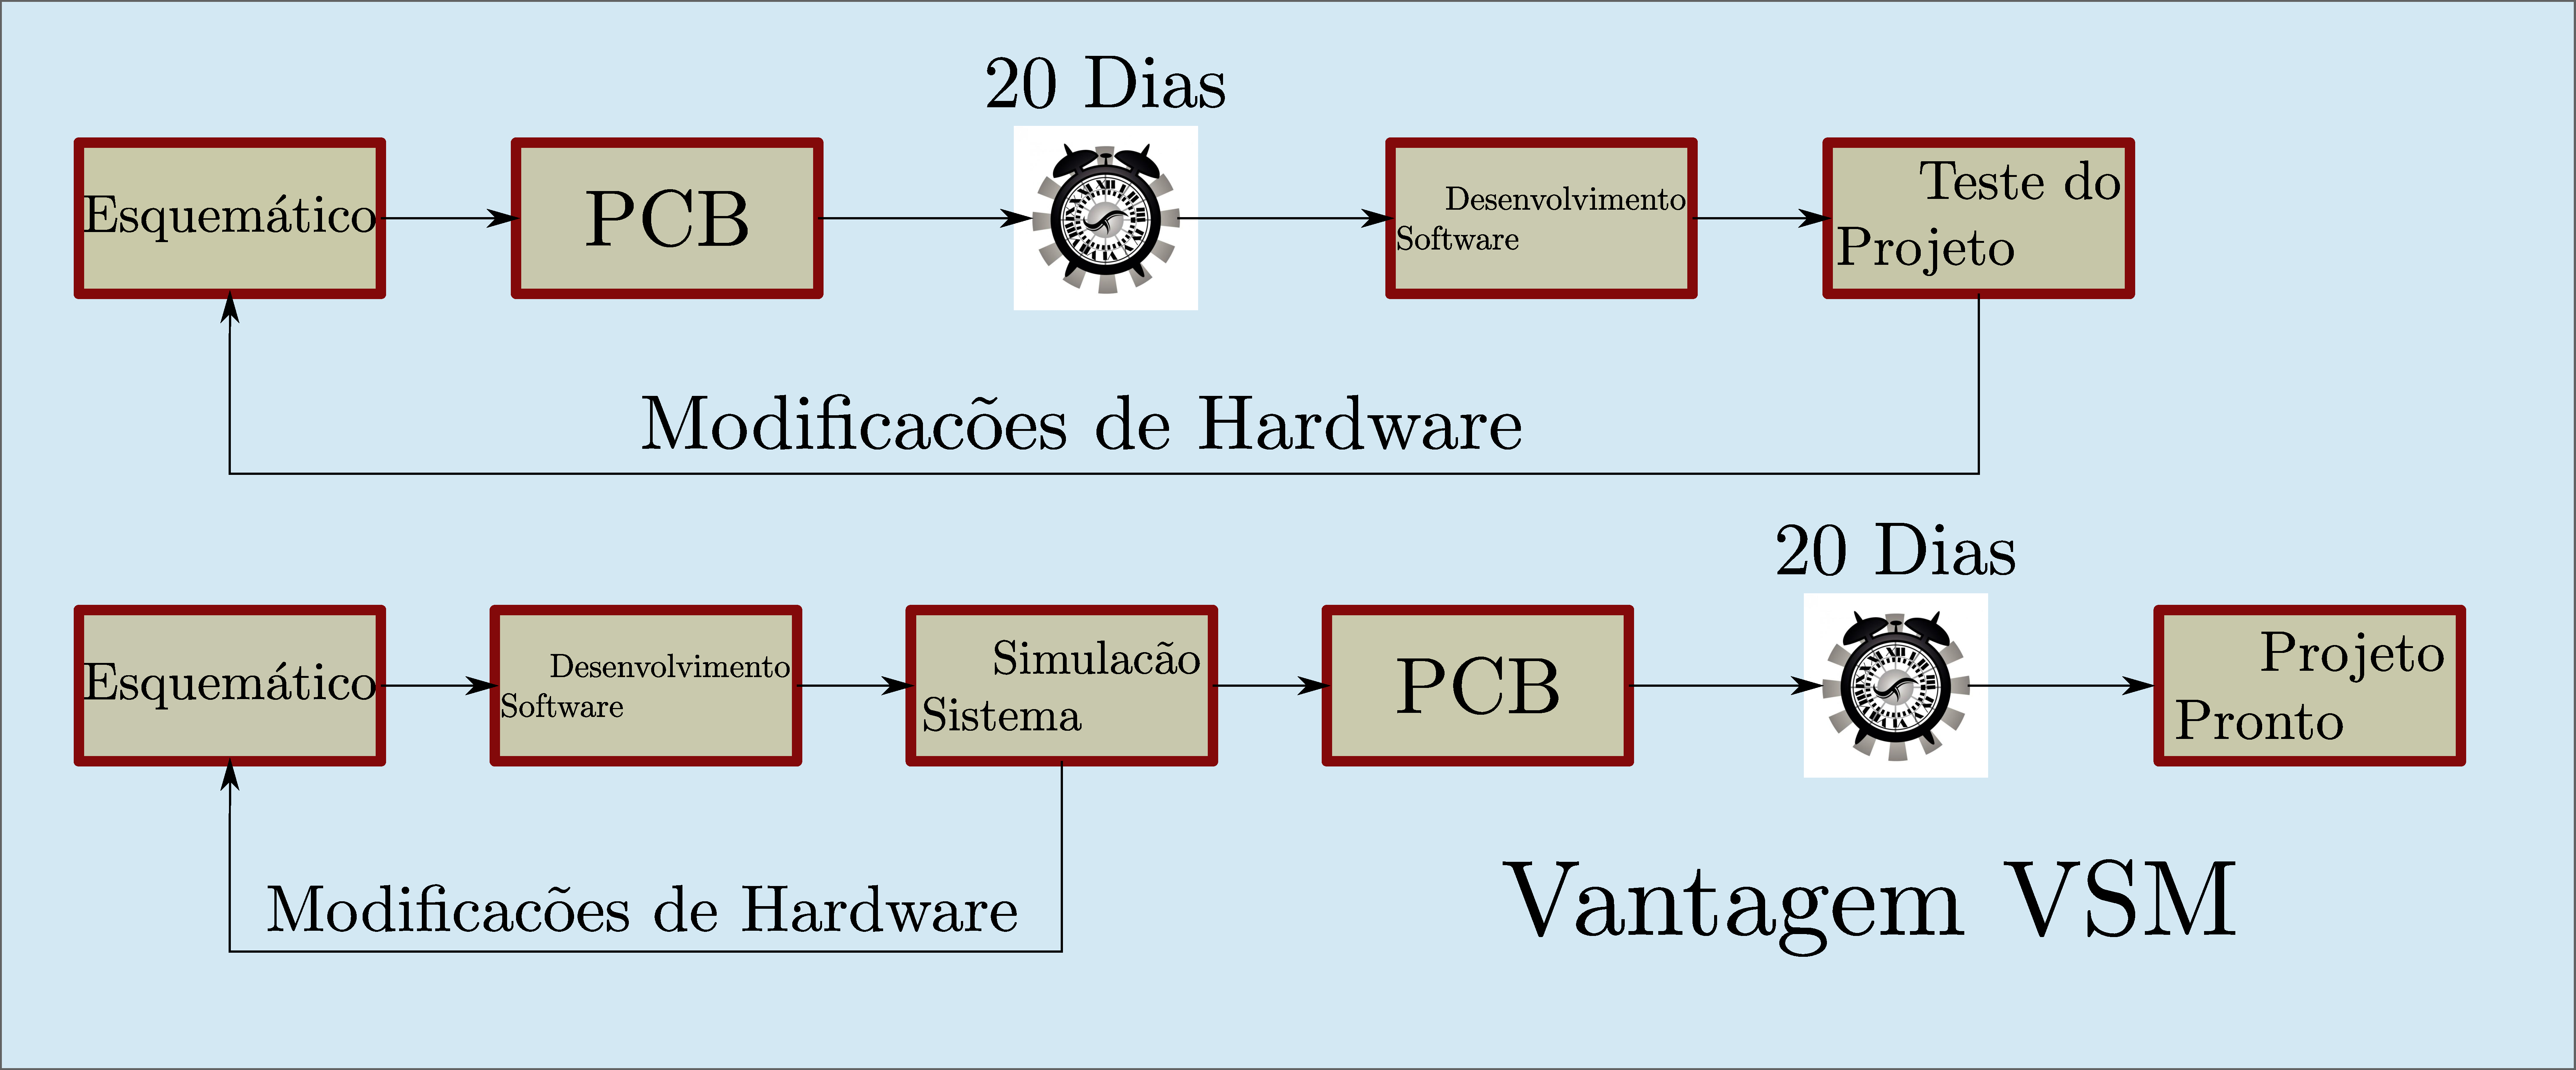
\includegraphics[width=1\textwidth]{Simulacao_proteus_esquematico_PCB.pdf}
\caption{VSM Proteus Vantagem de Uso}
\label{fig:Simulacao_proteus_esquematico_PCB}
\end{figure}

\pagebreak

\subsection{Proteus Interface}
\begin{figure}[h!]
\centering
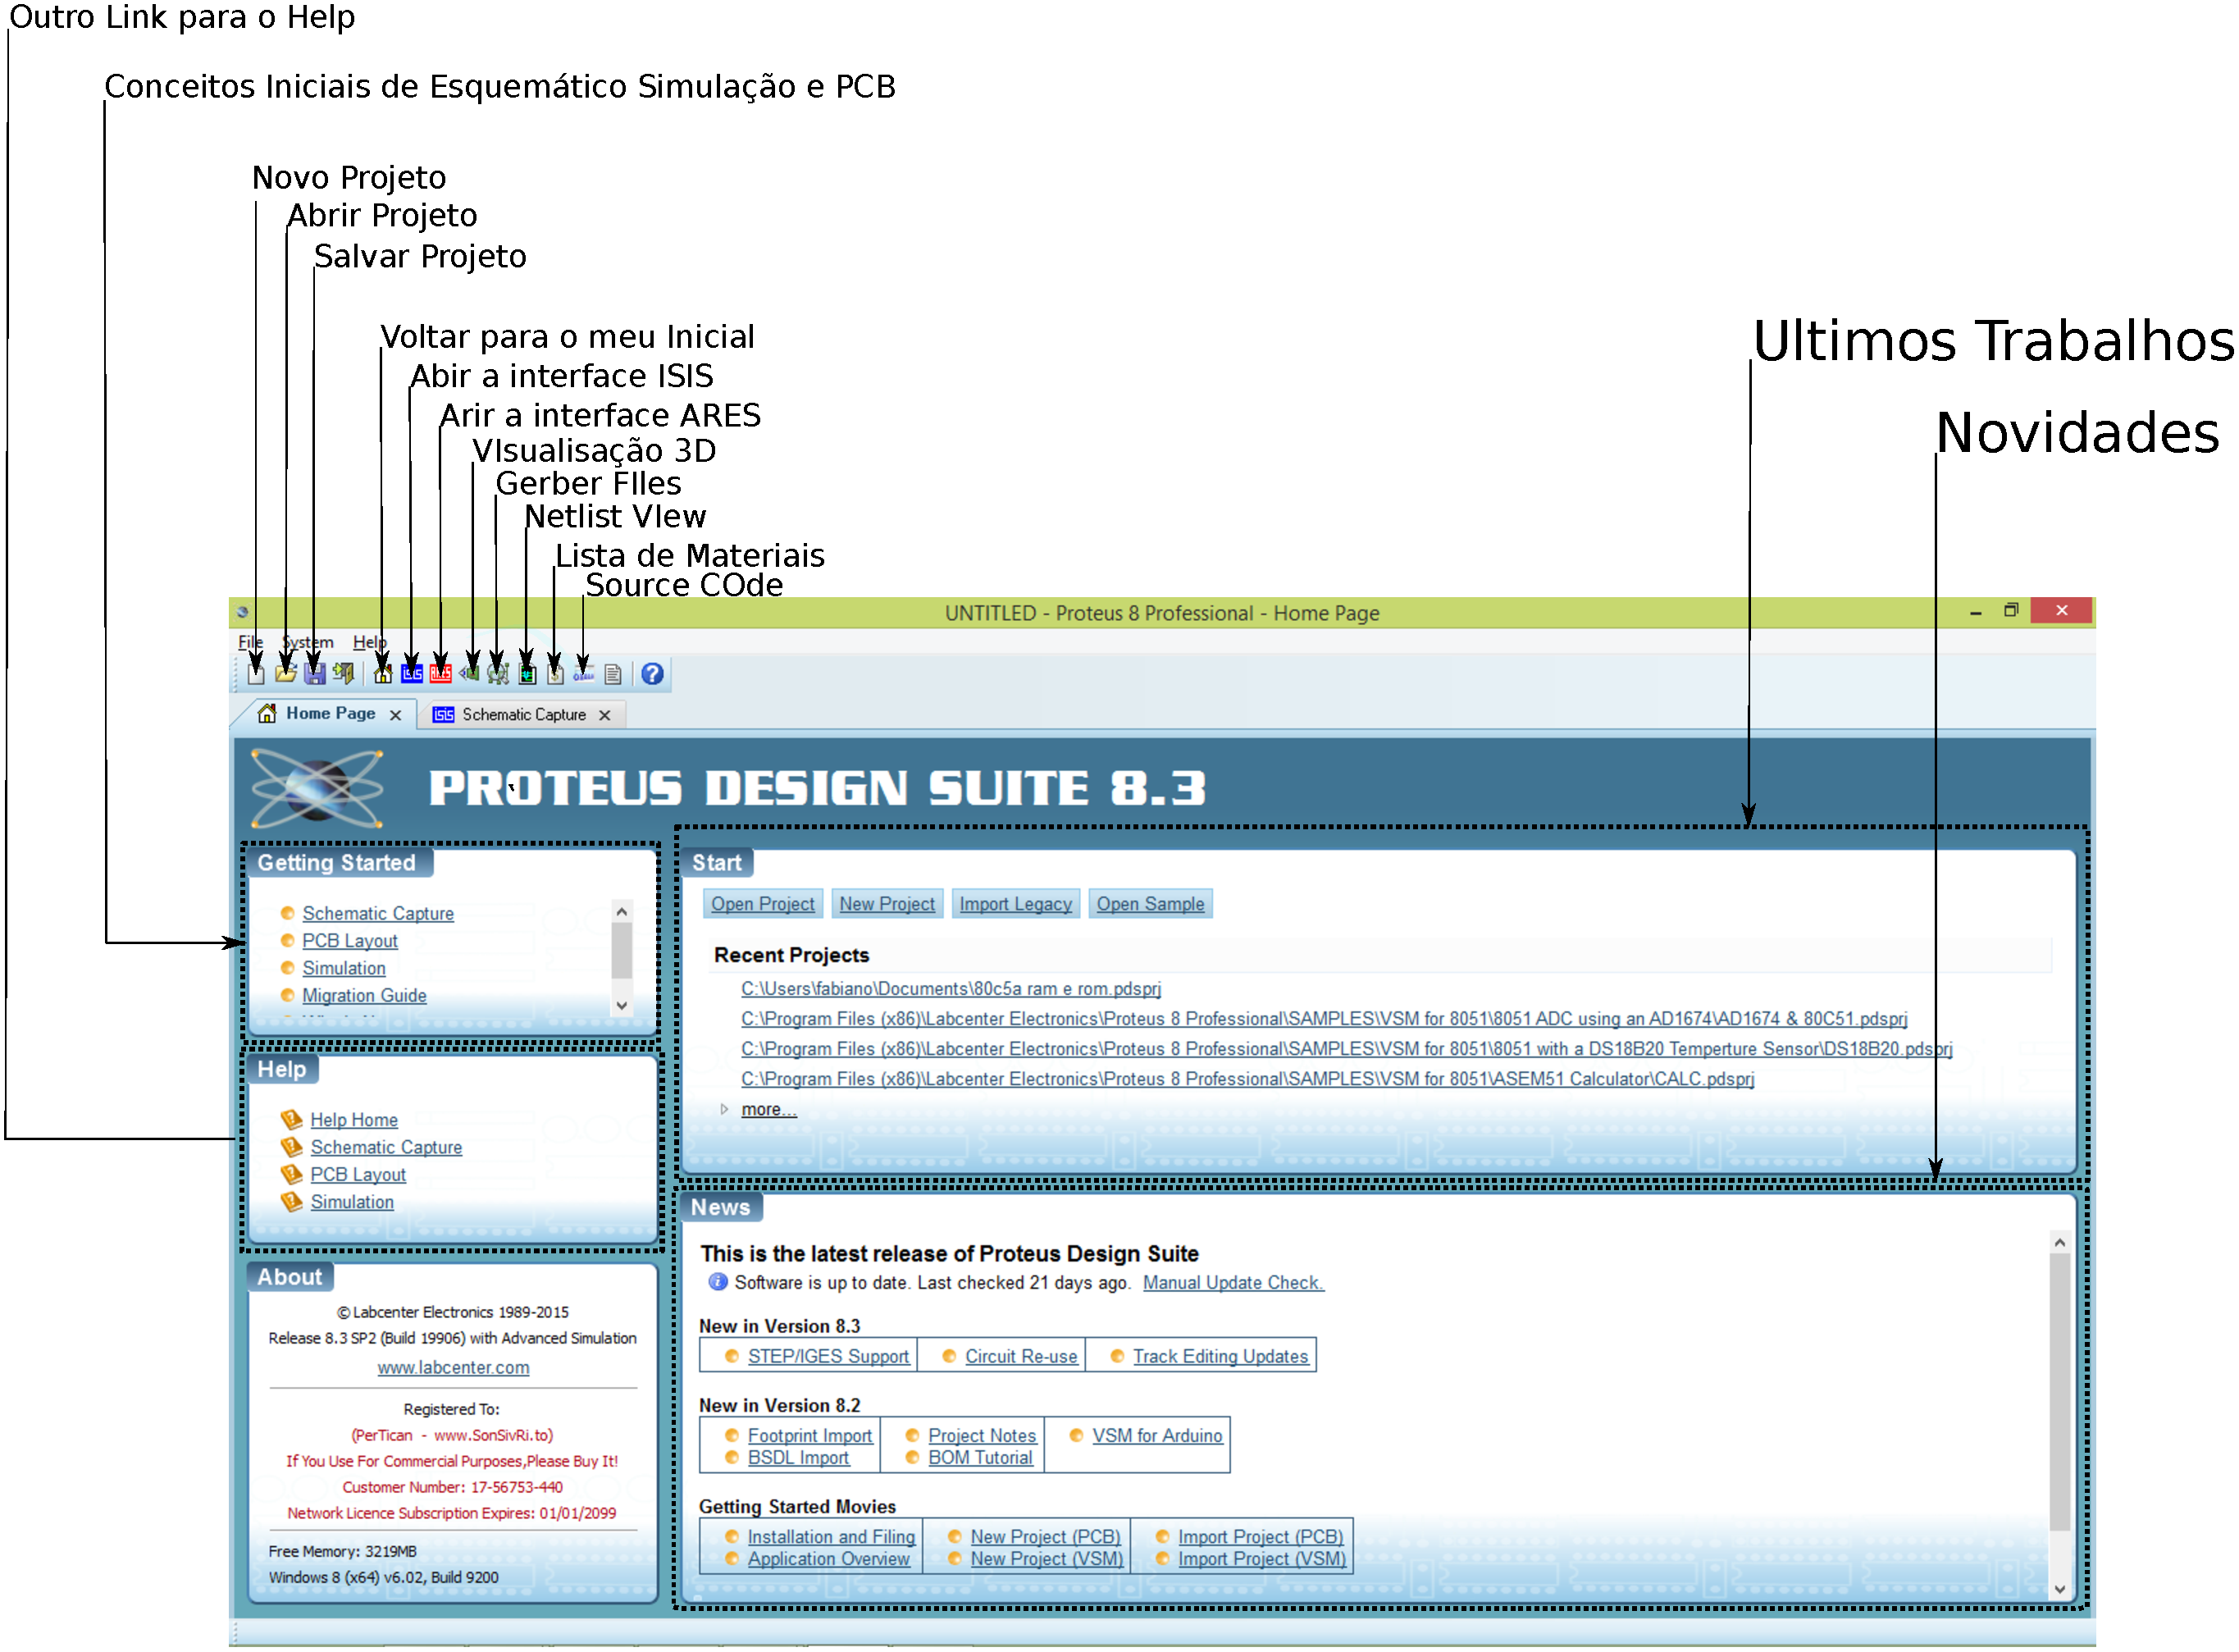
\includegraphics[width=1\textwidth]{Tela_Inicial.pdf}
\caption{Tela Inicial Proteus}
\label{fig:Tela_Inicial}
\end{figure}

\begin{itemize}
 \item \textbf{Outro link para o help} O help pode ser acessado por dois links, um pela janela indicada o outro pelo sinal de interrogação 2 
 itens ao lado de \textbf{Source Code}.
 \item \textbf{Conceitos iniciais de esquemático e simulação e PCB} Contem informações acerca dos itens citados, PCB, simulação e esquemático.
 Servindo como se fosse
 iniciais a serem exemplificado pelo software.
 \item \textbf{Novo Projeto} Inicia um novo projeto com opções de escolher o firmware se for desejado e outras configurações tais 
 layout do papel de esquemático
 e a possibilidade do emprego de PCB's de arduinos se o desejo do projetista é criar shields para essa plataforma.
 \item \textbf{Abrir Projeto} Escolha de um projeto pronto em algum diretório.
 \item \textbf{Salvar Projeto} Salva o projeto que foi iniciado.
 \item \textbf{Voltar ao Menu Inicial} Volta  para a interface expressa na figura(\ref{fig:Tela_Inicial}).
 \item \textbf{Abrir a Interface ISIS} Abre a interface que possibilita a construção e simulação do esquemático.
 \item \textbf{Abrir a interface ARES} Abre a interfaçe que possibilita a construção do PCB.
 \item \textbf{Visualização 3D} Visualiza o modelo real da placa renderizada no modo 3d.
 \item \textbf{Gerber Files} Gera os arquivos que após a construção do modelo PCB serão usados na confecção do produto gerado.
 \item \textbf{Netlist View} Verifica as ligações presentes no esquemático.
 \item \textbf{Lista de materiais} Após a confecção do equemático pode ser gerado uma lista de materiais que descrevem oque foram usados no esquemático.
 \item \textbf{Source Code} Para simulações aonde há a presença de microcontroladores pode-se , diretamente do proteus colocar o código de funcionamento do 
 microcontrolador.
 \item \textbf{Ultimos Trabalhos} Lista dos ultimos trabalhos acessados pelo programa.
 \item \textbf{Novidades} Novidades do da versão corrente do programa em relação aos anteriores.
 \end{itemize}

 
\pagebreak

\subsection{Proteus ISIS Interface}

\begin{figure}[h!]
\centering
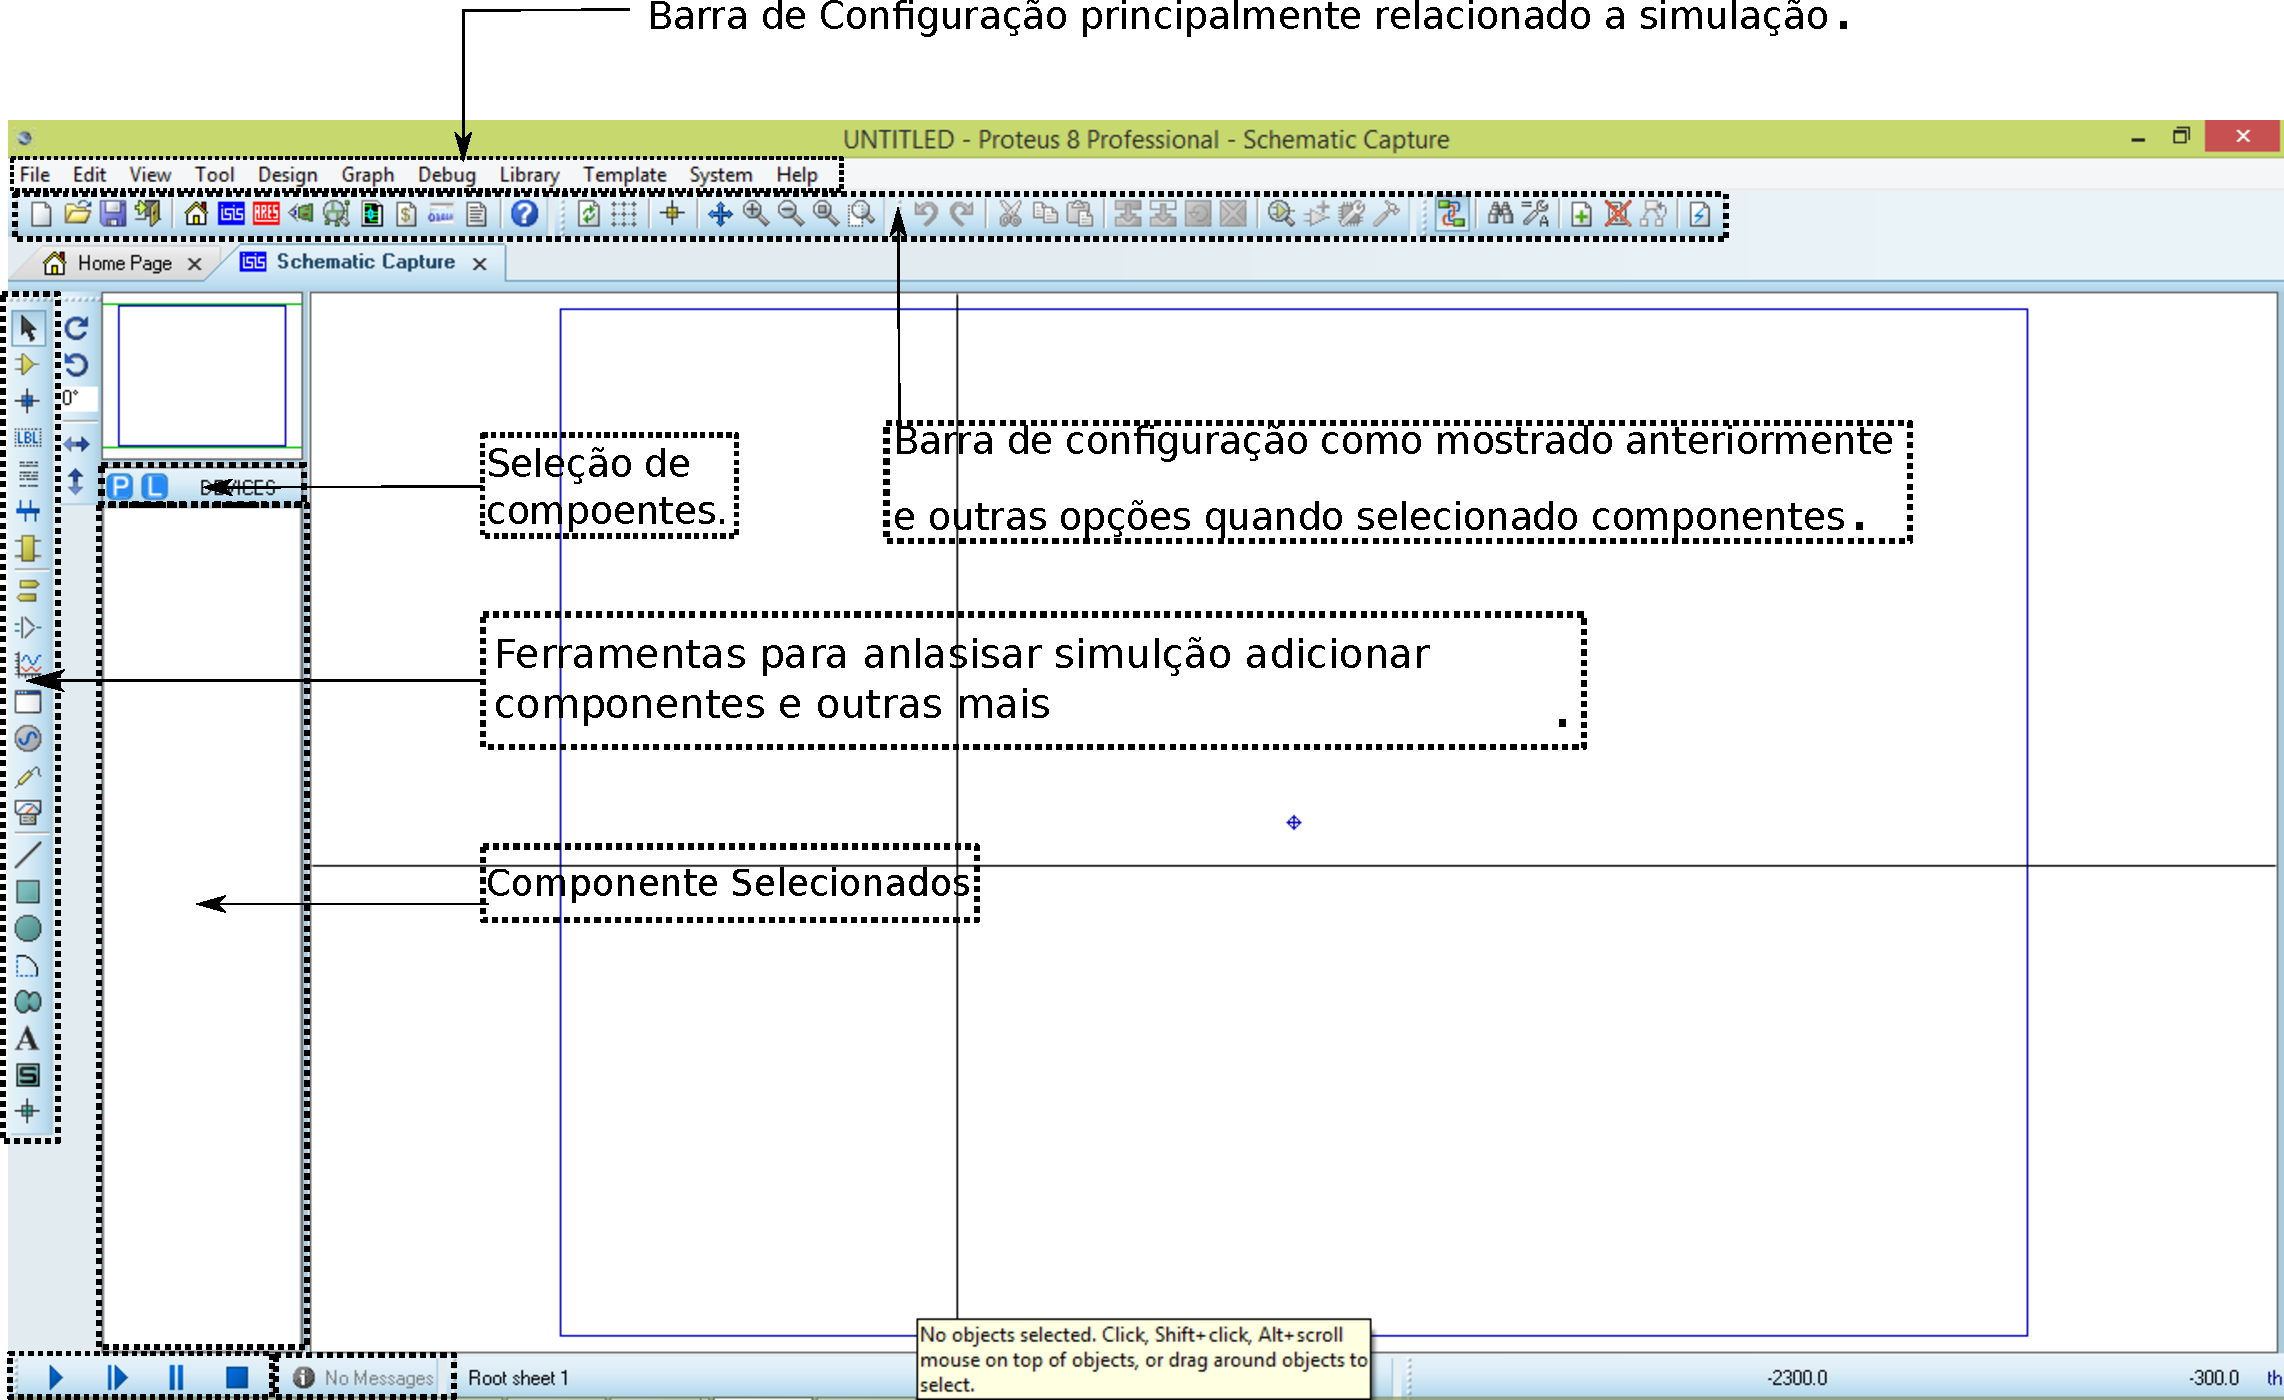
\includegraphics[width=1\textwidth]{tela_inicial_isis.pdf}
\caption{Tela Inicial Proteus ISIS}
\label{fig:tela_inicial_isis}
\end{figure}

Explicando os conceitos relacionado as possiveis opções a se escolher na pagina inicial do proteus, resta algumas opções a se explicar quando se esta na plataforma 
ISIS.

\begin{itemize}
 \item \textbf{Componentes Selecionados} Mostram os componentes que já foram adicinados a lista da onde podem ser retirados e colocados no esquemático.
 \item \textbf{Ferramentas para analisar simulação adicionar componentes dentre outras funcionalidades} Nesta seção há a possibilidade de adicionar ao esquemático
 ferramentas de verificação de simulação tanto no VSM como na simulação não animada.Cursor, seleção de componentes, centralização de imagem em um ponto, adição de
 bus para a criação de duto de dados, criação de componentes , seleção de ground e power 5v são a função das 8 primeiras possibilidades.\\
 Após estes simbolos encontra-se o  de simulação não animada tendo diversas possibilidade de simulação analógica ou digital.Letras e formas de figuras também 
 são adicionados por essa barra.
 \item \textbf{Seleção de Componentes} O P significa pick new component e o L Library são dois modo de se procurar componentes um por bibliotecas e outras 
 escolhendo pelo nome e ir filtrando pelas possibilidades de biliotecas e caracteristíca do componente a ser escolhido.
 \item \textbf{Barra de configuração dispensa comentários devido a imagem anterior}
\end{itemize}

\pagebreak

\section{Simulação 80c51 Assembler}
As simulações presentes neste documento baseam-se nas disciplinas Aplicação de Microprocessadores 1 e 2 sendo que o mesmo inicia-se em programação utilizando 
a linguagem assembler e a 
subsequente simulação no sistema via ISIS de todos os projetos.Assim o código será descrito via fluxograma e subsequente esquemático, com os resutados, ou 
somente esquemático que simula o programa. Na próxima seção todos os programas serão simulados em C.\\

\subsection{Práticas Botões e Leds}

As práticas consistem em simular o comportamento de leds com relação a chaves ligadas na porta P3, nos respectivos pinos P3.5, P3.6 e P3.7, ligando leds de
modos diferentes conforme o botão pe apertado, estando os leds na porta P1, respectivamente P1.1, P1.2 e P1.3.Isto e indicado na figura (\ref{fig:pratica_led_e_botoes}) 
sendo o esquemático do 8051 junto aos botões e leds. 

\begin{figure}[h!]
\centering
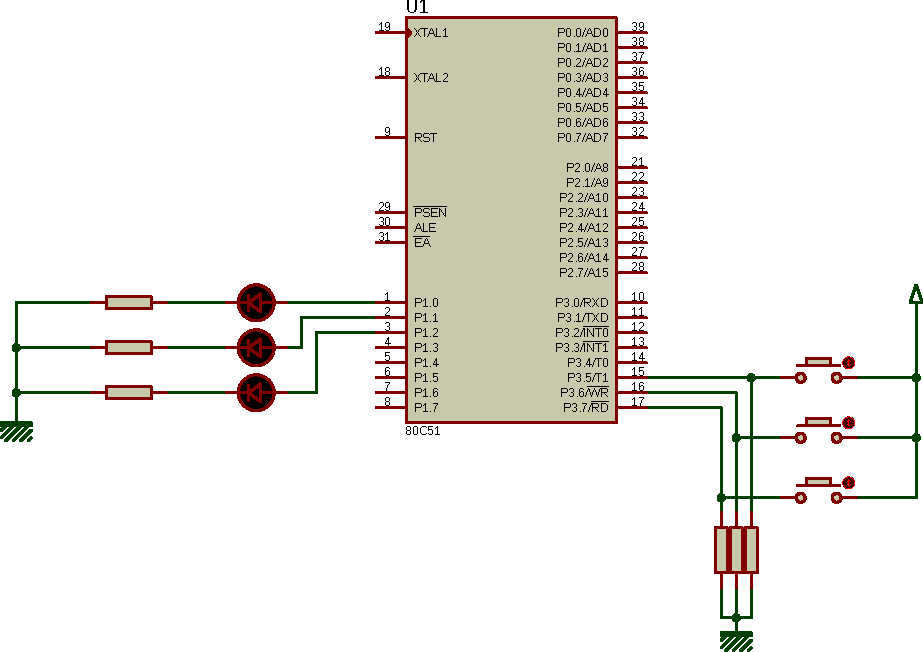
\includegraphics[width=.9\textwidth]{pratica_led_e_botoes.pdf}
\caption{Esquemático de Simulação Exercício Botões e Leds}
\label{fig:pratica_led_e_botoes}
\end{figure}

\pagebreak

O fluxograma que representa a programação do problema proposto encontra-se na figura (\ref{fig:fluxograma_exercicio1}) abaixo.

\begin{figure}[h!]
\centering
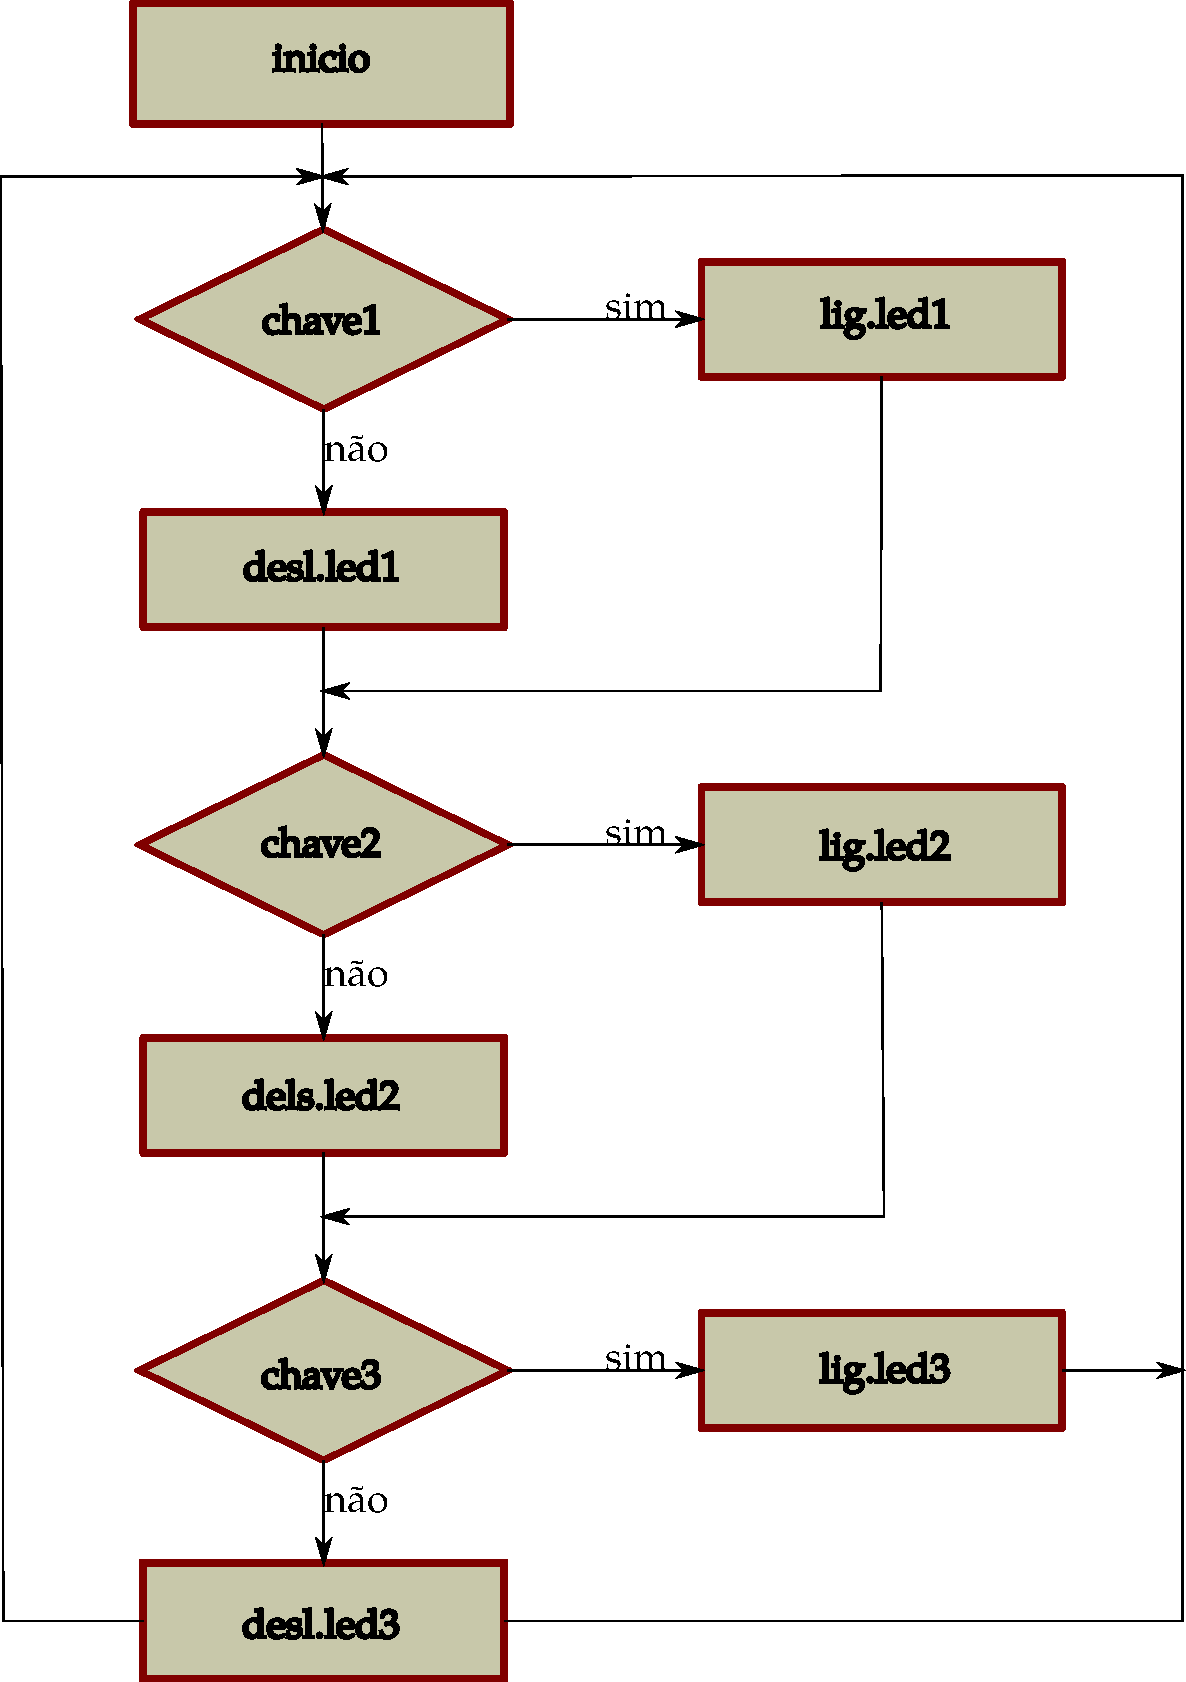
\includegraphics[width=.5\textwidth]{fluxograma_exercicio1.pdf}
\caption{Fluxograma do exercício 1}
\label{fig:fluxograma_exercicio1}
\end{figure}

O problema tem três possibilidades de elaboração, uma é essa expressa na figura (\ref{fig:fluxograma_exercicio1}) outra delas é a listada acima no fluoxograma
que acende o led correspondente conforme a chave ligada.Ainda é proposta para essa configuração como exercício os itens presentes abaixo.

\begin{itemize}
 \item Acender piscar cada led na frequência de 1 Hz para cada chave ligada correspondete ao mesmo.
 \item Acender um led com a chave1, outro led com a chave2 e piscar o led1 e led3 com a chave3 ligada, na frequência correspondente de 1 Hz cada led.
 \textbf{Atenção} Ligar os leds somente se a chave3 não estiver fechada.
 \end{itemize}

 
 \pagebreak
 
 Abaixo na figura (\ref{fig:exercicio2_simulacao}) encontra-se a simulação do exercício proposto no segundo item mostrando que piscam os leds na frequência de 
 1 Hz cada quando a chave3 esta pressionada. 
 
\begin{figure}[h!]
\centering
\includegraphics[width=.9\textwidth]{exercicio2_simulacao.pdf}
\caption{Simulação Exercício 2}
\label{fig:exercicio2_simulacao}
\end{figure}

\pagebreak

\subsection{Simulação Memória Ram e Rom Externas}
As memórias ram e rom externas podem fazer-se necessárias em projetos mais robustos, aonde exige-se mais armazenamento de dados do que a familia de 
microcontroladores oferece, que no caso, da 80c5x varia de 128 bytes de ram a 512 bytes e rom de 4 Kbytes a 32 Kbytes.Fazendo a expansão é possível endereçar 
até 64kbytes de ram externa e rom, e com outros modos, é possível também aumentar ainda mais essa possibilidade utilizando um shift-register como selecionador 
de memórias.Este ultimo modo não é coberto neste trabalho.\\
Para acessar os conteudos das memórias ram, em assembler no caso, considerando o compilador \textbf{MCU IDE 8051} é preciso usar os comando MOVX A,@A+DPTR
para acessar um valor externo ao microcontrolador que está endereçado no valor incluso no DPTR, e para colocar um valor no endereço apontado pelo DPTR é usado o
comando MOVX @DPTR,A. A memŕoria rom também tem comandos simples, bastando usar no lugar de MOVX o MOVC. Lembrando que faz-se somente leitura da rom e 
usa-se somente o comando MOVC A,@A+DPTR.O pino EA do micro deve estar ativo para acessar a memória rom externa, devendo haver atenção com este aspecto de esquemático\\
Assim, sendo simples os comandos, é importante focar no hardware que as operações exigem, afinal o funcionamento depende da montagem peculiar do esquemático,
iniciando uma ideia bastante importante do 80c51 que é a utilização do duto de dados presente na porta P0 como demultiplexada entre endereços e dados.O duto de 
endereços se estende até a porta P2, totalizando 16 bits de endereçamento oque possibilita uma expansão de até 64k de memórias.\\
Se caso não for usado todos os bits de endereçamento, os restante são usados como seleção fazendo uma regra em que cada endereço alocado selecione um componente,
por um chip chamado decodificador.O esquemático pode ser visto na figura (\ref{fig:ram_rom}) com o microcontrolador uma memória ram de 8k e uma rom de 8k.\\
É importante salientar o uso dos probes na simulação, eles permitem verificar o valor de um dado pino em um dado instante, havendo a possibilidade de simulações
digitais, ou mixas, oque será visto mais adiante.Há a possibilidade de se verificar qual o conteúdo de um duto, apenas utilizando os probes e o bus-wire, crucial
na montagem de esquemas afinal este diminui bastante a desorganização do esquemático, porém torna mais minuciosa a construção, afinal cada ligação precisa estar
corretamente nomeada.

\begin{figure}[h!]
\centering
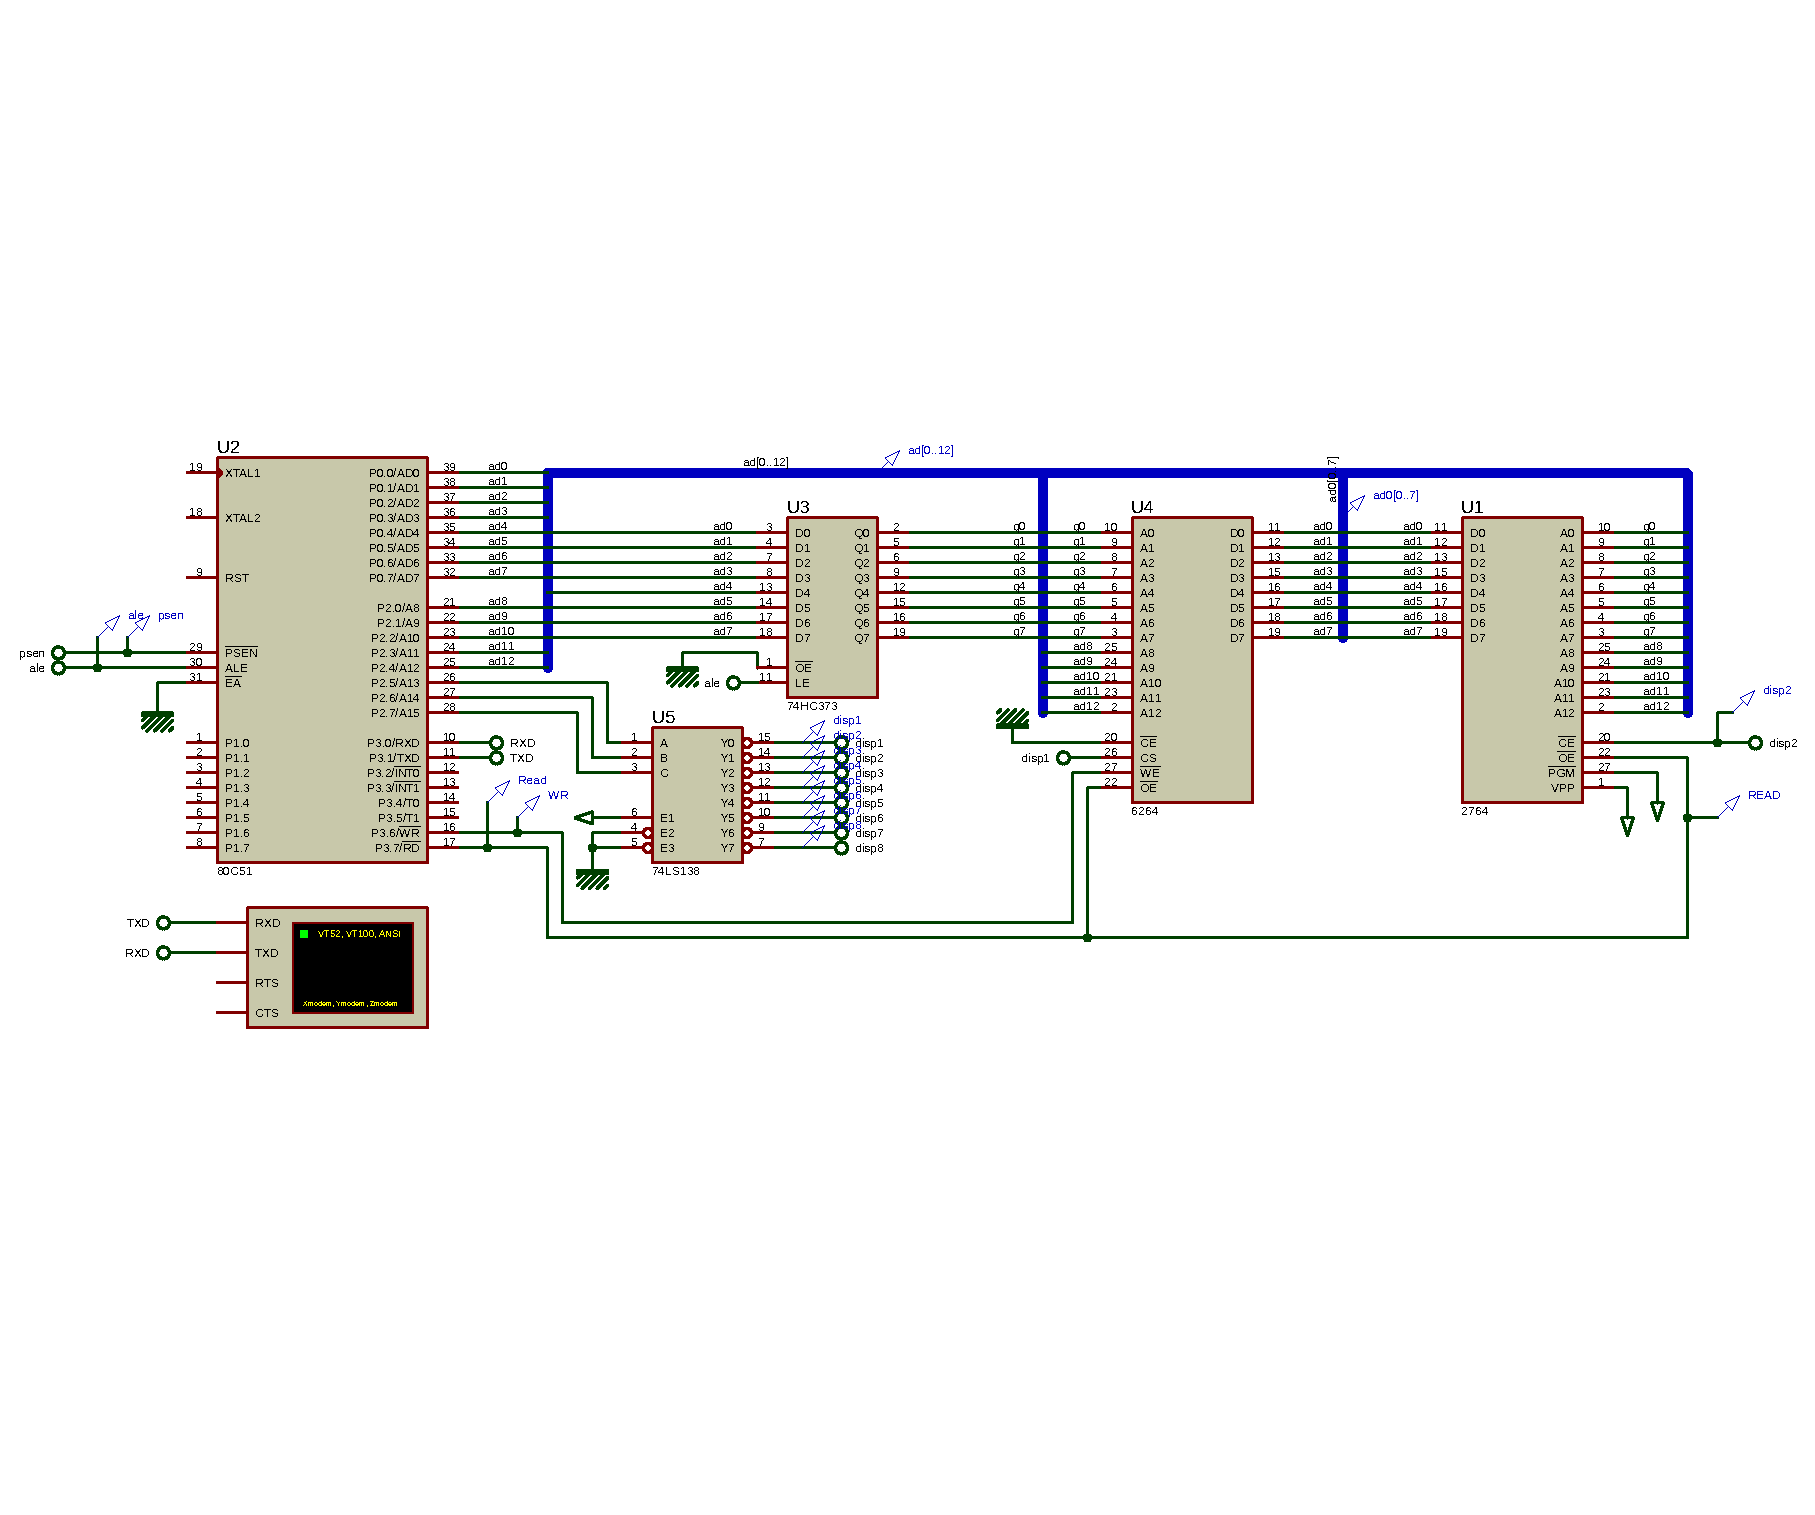
\includegraphics[width=1\textwidth]{ram_rom.pdf}
\caption{Hardware Ram e Rom de 8Kbytes}
\label{fig:ram_rom}
\end{figure}

Foi feito um programa que varre o DPTR de 0000h a ffffh e coloca um valor de 00h a ffh na memória ram.Além disso verifica os pinos de seleção, que são ativos em 
zero.Como a mémoria é de 8K, há a necessidade de 13 pinos do microcontrolador para conectá-las, sobrando, ao fim, 3 pinos para seleção, o que torna possível a 
utilização de um decodificador para endereçar 8 elementos. O resultado da simulação encontram-se nas figuras (\ref{fig:ram_rom_varrendo_tudo}) 
e (\ref{fig:ram_e_rom_duto_conteudo}) uma mostrando a simulação por completo e a outra especificando, em um dado momento, o dado passando pelo duto de dados 
e de endereços.

\newpage

\begin{figure}[h!]
\centering
\includegraphics[width=0.89\textwidth]{ram_rom_varrendo_tudo.pdf}
\caption{Varrendo Todos os Valores do DPTR}
\label{fig:ram_rom_varrendo_tudo}
\end{figure}

\begin{figure}[h!]
\centering
\includegraphics[width=0.89\textwidth]{ram_e_rom_duto_conteudo.pdf}
\caption{Selecionando Valores Vizualizaveis do DPTR}
\label{fig:ram_e_rom_duto_conteudo}
\end{figure}

\newpage

Verifica-se, na simulação acima, figura (\ref{fig:ram_e_rom_duto_conteudo}) que no valor 080Ch do DPTR é colocado o valor DCh e assim sucessivamente, incrementando
o DPTR e o valor a ser colocado na memória.Verifica-se também que o dispositivo selecionado no momento da operação é o dispositivo 7, afinal seu valor vai para
zero quando colocado o valor no duto de dados, enquanto todos os demais fica em nível alto no momento da alocação de dados.\\
Essa maneira de pensar , selecionando objetos e trabalhando somente com o selecionado, como já foi dito, é muito importante para o 80c51.\\

\pagebreak

\subsection{Comunicação Serial}
Pode-se fazer comunicação serial de dados, oque significa enviar um bit por vez, partindo do emissor para o receptor, sendo que desses bits alguns sinalizam
o caracter e outros que significam informações de parada, inicio de comunicação dentre outros conforme  a configuração da comunicação.\\
Neste documento foram realizadas as comunicações seriais de 8 bits de caracter e um de inicio, que pode ser configurado no 80c51.Interessante resaltar 
que há possibilidade de uma comunicação serial com o 80c51 se da devido ao mesmo possuir uma UART como hardware em sua arquitetura.\\
A taxa BAUD-RATE de comunicação serial, sendo a quantidade de bit enviada por segundo pelo terminal de comunicação, foi taxada como sendo de 9600($\frac{bits}{s}$ 
porém pode-se configurar o microcontrolador para realizar comunicações com outros BAUD-RATE, lembrando que no proteus a configuração deve ser feita tanto em software 
como em hardware, modificando no terminal serial, mostrado na figura ({\ref{fig:serial_80c51}) abaixo.

\begin{figure}[h!]
\centering
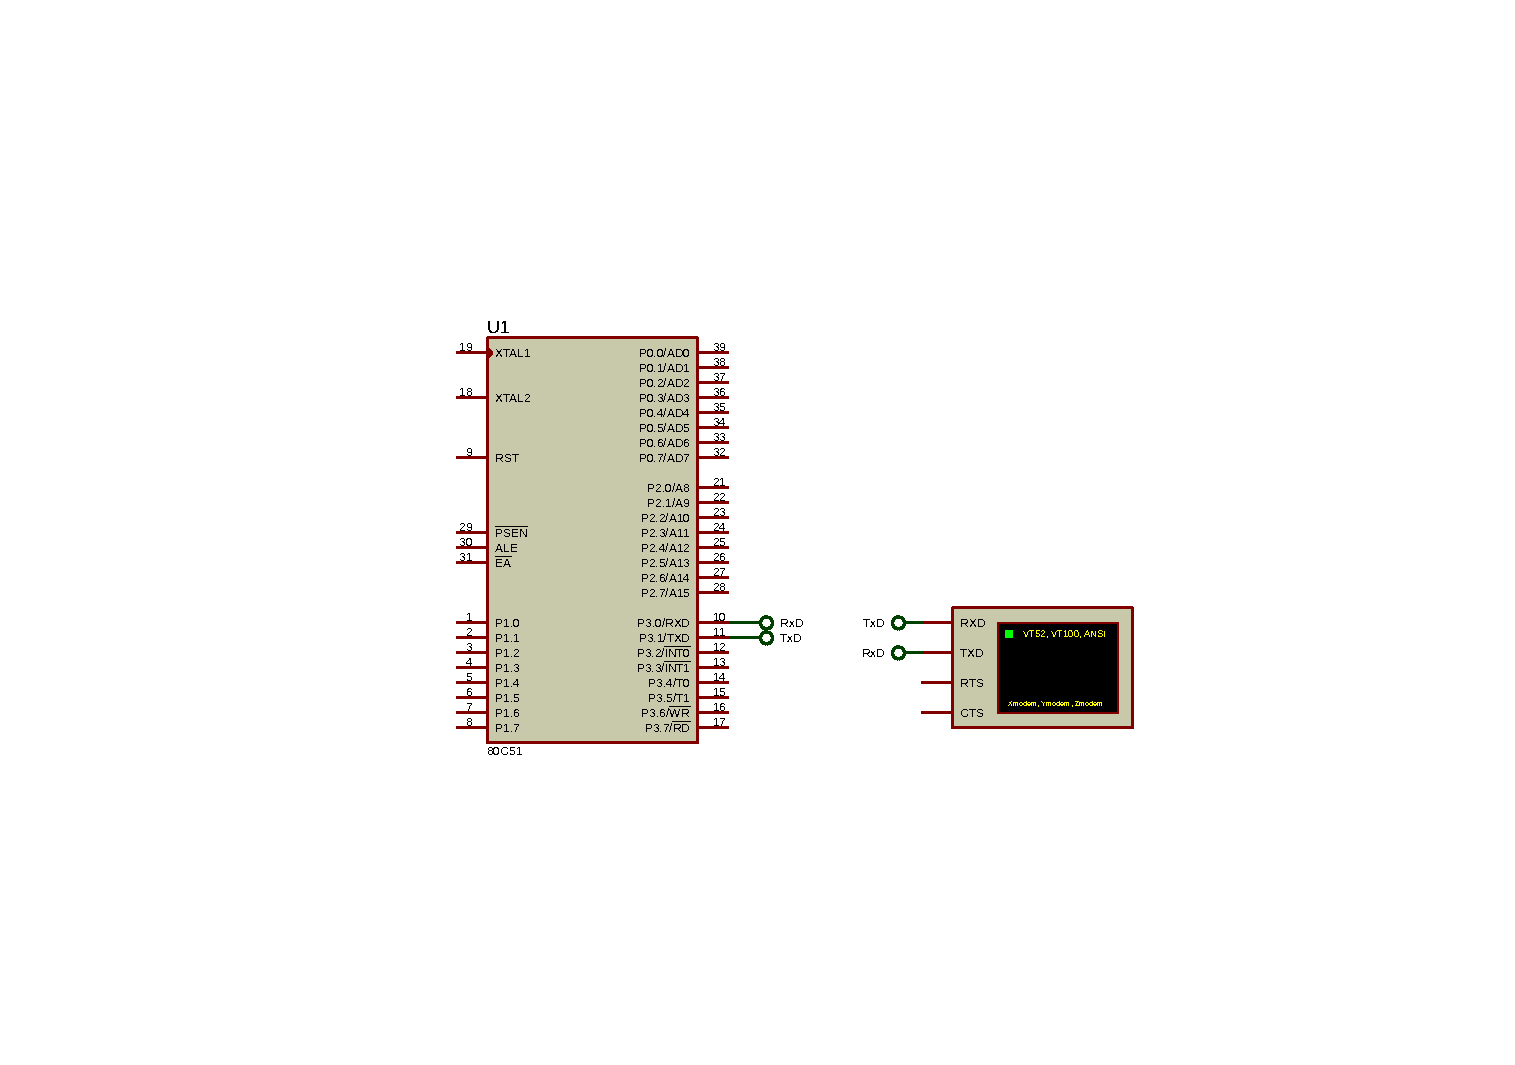
\includegraphics[width=1.2\textwidth]{serial_80c51.pdf}
\caption{Esquema de Hardware Para a Simulação da Comunicação Serial}
\label{fig:serial_80c51}
\end{figure}

\pagebreak

Há  as configurações de BAUD-RATE variando conforme protocolos de comunicação sendo dois bastante conhecidos de comunicação RS-232 e o RS-485.
Também pode-se configurar o microcontrolador para realização comunicação com diferentes quantidade de bits.Foram fixados 10 bits, e taxa de BAUD-RATE de 9600($\frac{Bits}{s}$).
A figura (\ref{fig:enviando_um_caracter_continuamente}) ilustra como se dá o comportamento dos bits da comunicação quando é enviado para o terminal serial.
O caracter enviado é o 'F'.

\begin{figure}[h!]
\centering
\includegraphics[width=0.95\textwidth]{enviando_um_caracter_continuamente.pdf}
\caption{Bits que Representam a Comunicação Serial do Caracter F}
\label{fig:enviando_um_caracter_continuamente}
\end{figure}

Como possibilidades de simulação ficam a critérios de escolha de configuração de outros valores de BAUD-RATE, e o iten listado abaixo:

\begin{itemize}
\item Fazer um programa que envia uma frase dependendo do caracter enviado, ainda contando com um caracter que imprima todas as frases armazenas.
\end{itemize}

\newpage

\begin{figure}[h!]
\centering
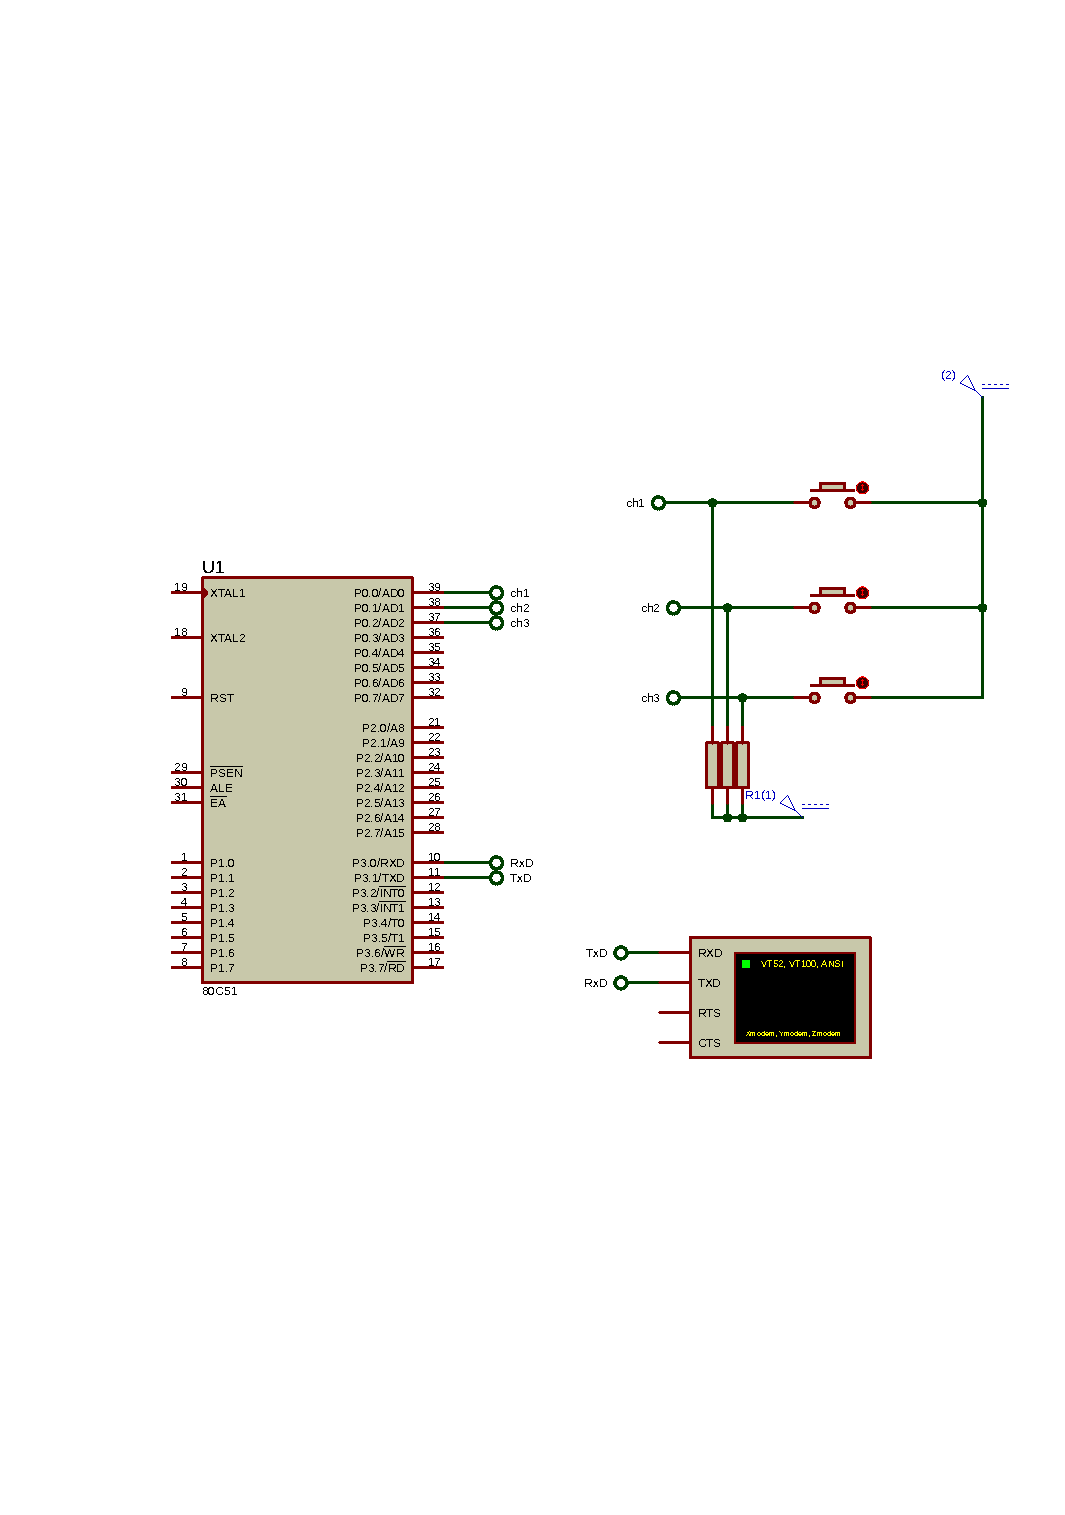
\includegraphics[width=0.95\textwidth]{botoes_serial.pdf}
\caption{Hardware Que Possibilita a Simulação de Envio de Frase Dependente de Botão.}
\label{fig:botoes_serial}
\end{figure}

\newpage

Abaixo na figura (\ref{fig:fluxograma__envio_de_caracter}) encontra-se o fluxograma que ilustra o envio continuo de um caracter.O envio de uma frase exige 
a utilização de um ponteiro que aponte para a frase fazendo com que o conteúdo do ponteiro seja passada para o registrador SBUF.
Assim, além de verificar se a transmissão de cada caracter é preciso identificar mais um if(cjne) verificando o fim do envio da frase.Para fazer as 
simulações com a interrupção bastam configurá-la, lenbrando que é preciso habilitar a recepção, por meio do bit REN.\\


\begin{figure}[h!]
\centering
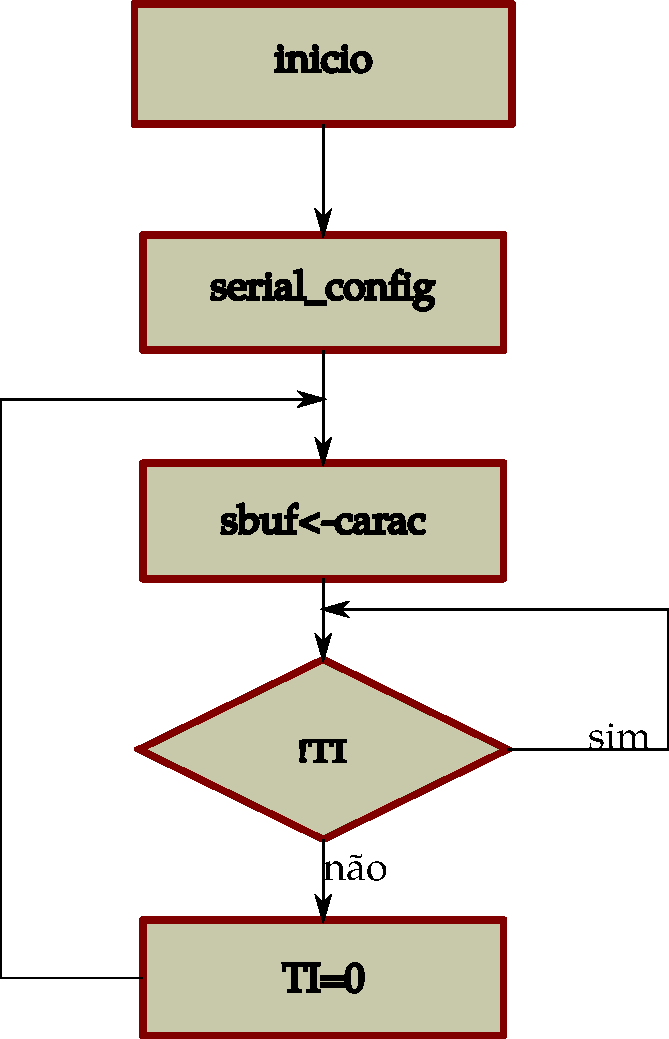
\includegraphics[width=0.3\textwidth]{fluxograma__envio_de_caracter.pdf}
\caption{Fluxograma do Recebimento de um Caracter sem Interrupção}
\label{fig:fluxograma__envio_de_caracter}
\end{figure}

\pagebreak

\subsection{Timers, Interrupções e Contadores : Projeto Conversor AD}
Dentre os elementos que constituem o microcontrolador 80c51 há dois timers de 16 bits cada e a presença de 5 tipos de interrupção,sendo uma delas extra.
Sempre que utilizá-las é preciso que se faça sua configuração e escolha conforme o trabalho a ser executado.\\

Os timers presentes são \textbf{timer1} e o \textbf{timer0} ambos de 16 bits configurados pelos registrados DPHx e DPLx sendo x 1 ou 0, correspondendo ao timer em 
questão.\\

As interrupções estão relacionadas aos hardwares com as quais funcionam, no caso de recepção e transmissão serial, ao bit de finalização da transmissão recepção
da serial.As externas relacionam-se com os pinos INT0 e INT1 e o overflow dos timers que se relacionam com bit TF, indicando estouro de contagem.\\

Como possibilidades de projeto pode-se fazer a geração de formas de ondas quadradas com qualquer dos timers utilizando um esquemático que seja apenas o 80c51
ou contar quanto tempo uma onda fica em nivel alto, utilizando o timer como temporizador, para isso basta que se faça a configuração do microcontrolador 
e adicione probes no esquemático para visualizá-la.Pode-se utilizar o oscilocópio disponível na barra de ferramentas, caso opte-se pela simulação animada.\\

Outra possibilidade de projeto é fazer um medidor de tempo em nível alto de uma onda e imprimir na serial, lembrando que será preciso fazer a conversão hexa asc 
do valor presente no contador.Além disso há o fato de que os timers são de dezesseis bits, o acumulador e registradores são de oito bits,
devendo retirar os valores dos registradores DPhx e DPLx.\\

O projeto do conversor AD não irá dar enfase em critérios de conversão, como precisão e se os tempos de amostragem estão satisfazendo os critérios de desempenho
da aplicação em questão, mas sim a utilização de uma maneira bastante prática o uso de interrupções, utilizando a interrupção de qualquer dos timers além de uma 
externa.

\subsubsection{Conversores e Breve Conversão AD e DA}
Conversão analógica digital envolve vários conceitos, como tempo de amostragem, resolução, tempo de conversão para limites de frequência que podem ser converti
dos.Isto será deixado de lado nesta análise, sendo o objetivo somente fazer funcionar o conversor AD, pegar o valor convertido e colocar em outra porta do microcontrolador
aonde está conectado um conversor DA, com a qual será feita comparação entre os sinais de entrada e de saída.\\

O esquemático que possibilita esta simulação encontra-se na figura (\ref{fig:adc_dac_ideal}) que trata-se do microcontrolador 80c51 junto a um conversor ADC0808 e DAC0808.Utilizando
geradores de onda do proteus para simular os cloks e pulso de start que encontra-se no esquemático citado.\\

O esquemático que simula o conversor AD junto ao microcontrolador, fazendo uso de uma fonte, um node de geração de pulsos, acessado na barra de ferramenta a 
esquerda no ISIS, cujos valores são 680k para o clok e 5k para o start é o mesmo citado anteriormente.A programação do micro é apenas colocar na porta P2 
o valor convertido que encontra-se na porta P1, enfim o código faz P2=P1.Em P1 encontra-se um conversor AD, que converter para analógico o sinal digitalizado.
Na figura (\ref{fig:adc_8051_dac_ideal}) encontra-se a simulação da conversão ad realizada.

	\newpage
	%\thispagestyle{empty}
	\clearpage
	\begin{sidewaysfigure}
		\centering
		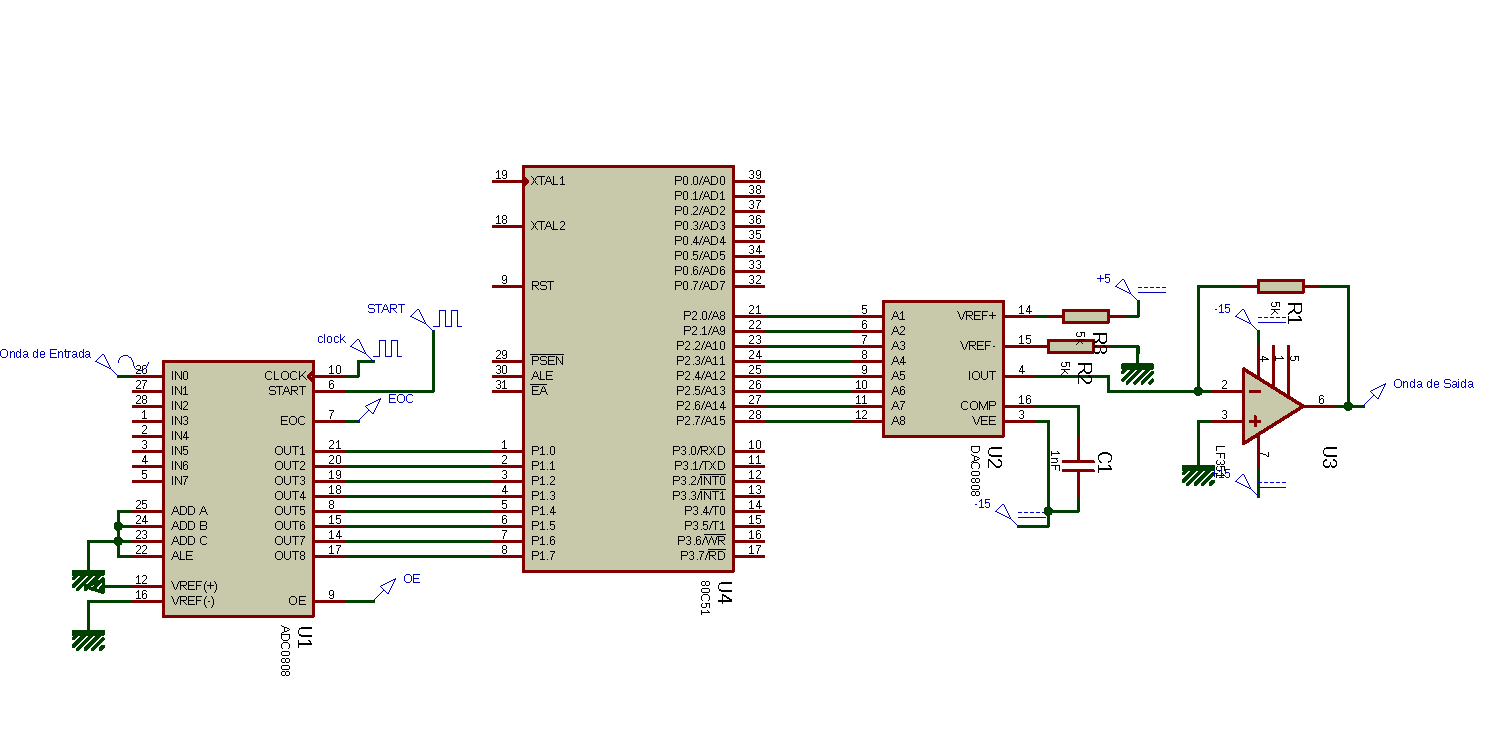
\includegraphics[width=1\linewidth]{adc_dac_ideal}
		\label{fig:adc_dac_ideal}
	\end{sidewaysfigure}
	%\clearpage
	%\pagenumbering{gobble}
	\newpage

\begin{figure}[h!]
\centering
\includegraphics[width=1\textwidth]{adc_8051_dac_ideal.pdf}
\caption{Simulação Conversores AD DA e 80c51}
\label{fig:adc_8051_dac_ideal}
\end{figure}

\newpage

\subsection{Conversor AD e DA Controlado Pelo 80c51}
È preciso que haja a leitura do datasheet do conversor ADC0808 e DAC0808 para verificar os valor que deve ser inserido como clock que 
não pode ser alcançado pelo micorontrolador 80c51 levando a necessidade de se trablahar em uma frequência mais baixa,além de carregar o 
timer no máxino fffeh, para que haja interrupção no seu estouro.Ao fim da conversão é gerado um pulso em nivel alto no pino EOC do conversor AD.
O conversor DA apenas converte para analógico o sinal digital, assim sua única limitação é quanto ao tempo de conversão, oque, para testes 
não significara muito caso sejam convertidos sinais de baixa frequência.\\

Assim, tem-se como objetivo gerar uma onda quadrada por meio da interrupção de um dos timers e configurar alguma interrupção externa sensível a borda de subida
do EOC, e dentro da interrupção ler o valor convertido.O fluxograma da figura (\ref{fig:adc_dac_80c51_fluxograma}) espressa o controle do conversor AD.
	

\begin{figure}[h!]
\centering
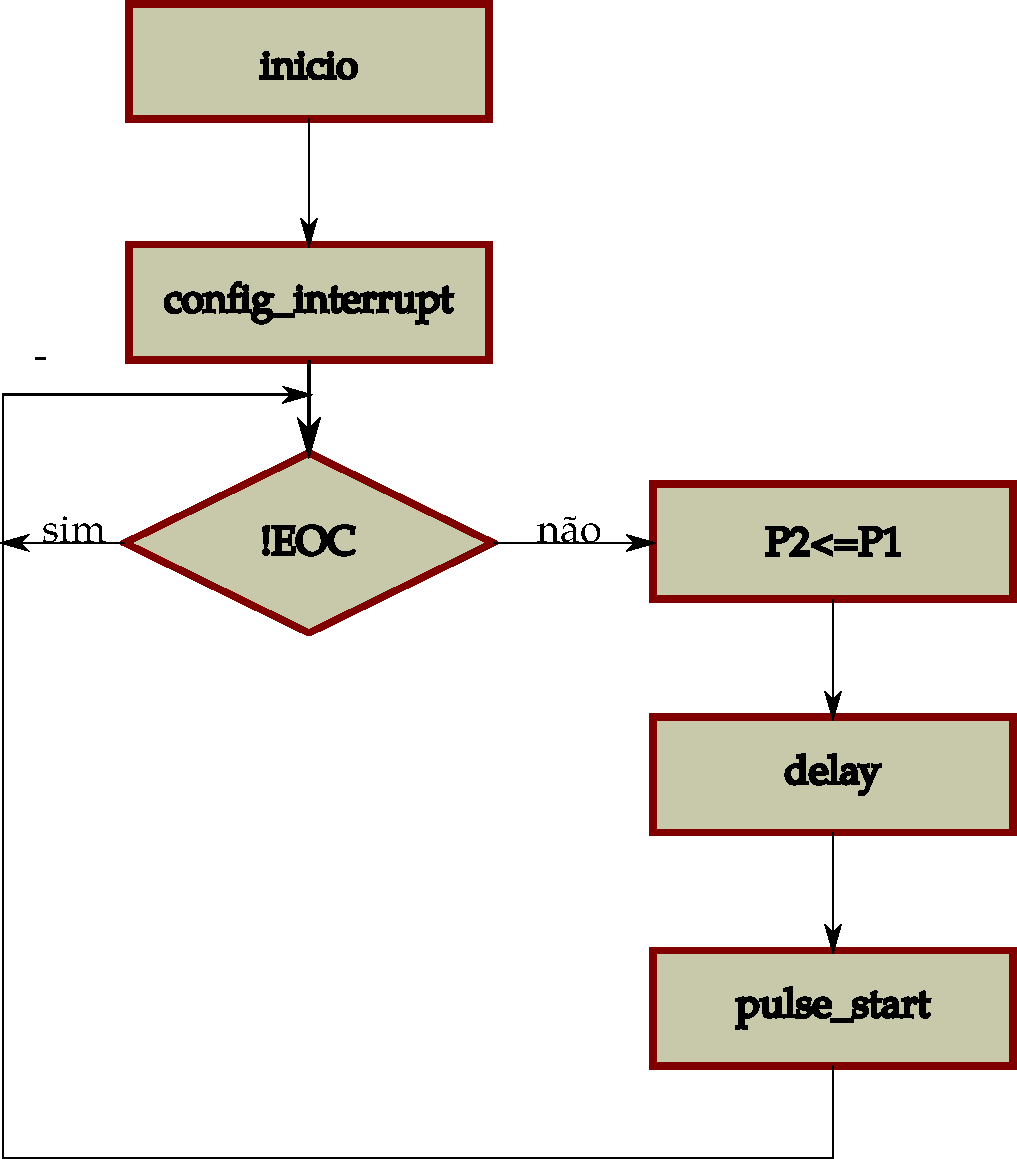
\includegraphics[width=.47\textwidth]{adc_dac_80c51_fluxograma.pdf}
\caption{Simulação Conversores AD DA e 80c51}
\label{fig:adc_dac_80c51_fluxograma}
\end{figure}

Verifica-se pelo datasheet do ADC0808 que o mesmo trabalha com clock tipico de 680kHz.Diz também que o pulso de start tem que ter duração maior que 
200ns e que o tempo de conversão será no valor de 90 a 100us.Dessa forma há a necessidade de se trabalhar com valores menores de clock e aumentar o 
pulso de start para controlá-lo por meio do 80c51 afinal nem carregando o timerx com fffeh não é um tempo minimo de overflow que gera 680kHZ.\\
	
Na simulação feita foi carregado timer1 com o máximo fffeH, inicia o timer1, espera 10us e da um pulso de start após isto espera o EOC ir para 1, acionando a 
interrupção.Na interrupção tirar o valor da P1 e passar para P2.Após isto reinicia-se o ciclo.\\
 
Na figura (\ref{fig:adc_dac_completa}) encontra-se o hardware que possibilita esta simulação.Deste modo tem-se o fluxograma e o hardware mínimo para simulação.
A figura (\ref{fig:adc_8051_dac}) expressa o resultado da conversor de uma forma de onda construida a mão pelo gerado pwlin.Além de desenhar a forma de 
onda é possível programa-la por meio da linguagem HDL.

	%\newpage
	%\thispagestyle{empty}
	%\clearpage
	\begin{sidewaysfigure}
		\centering
		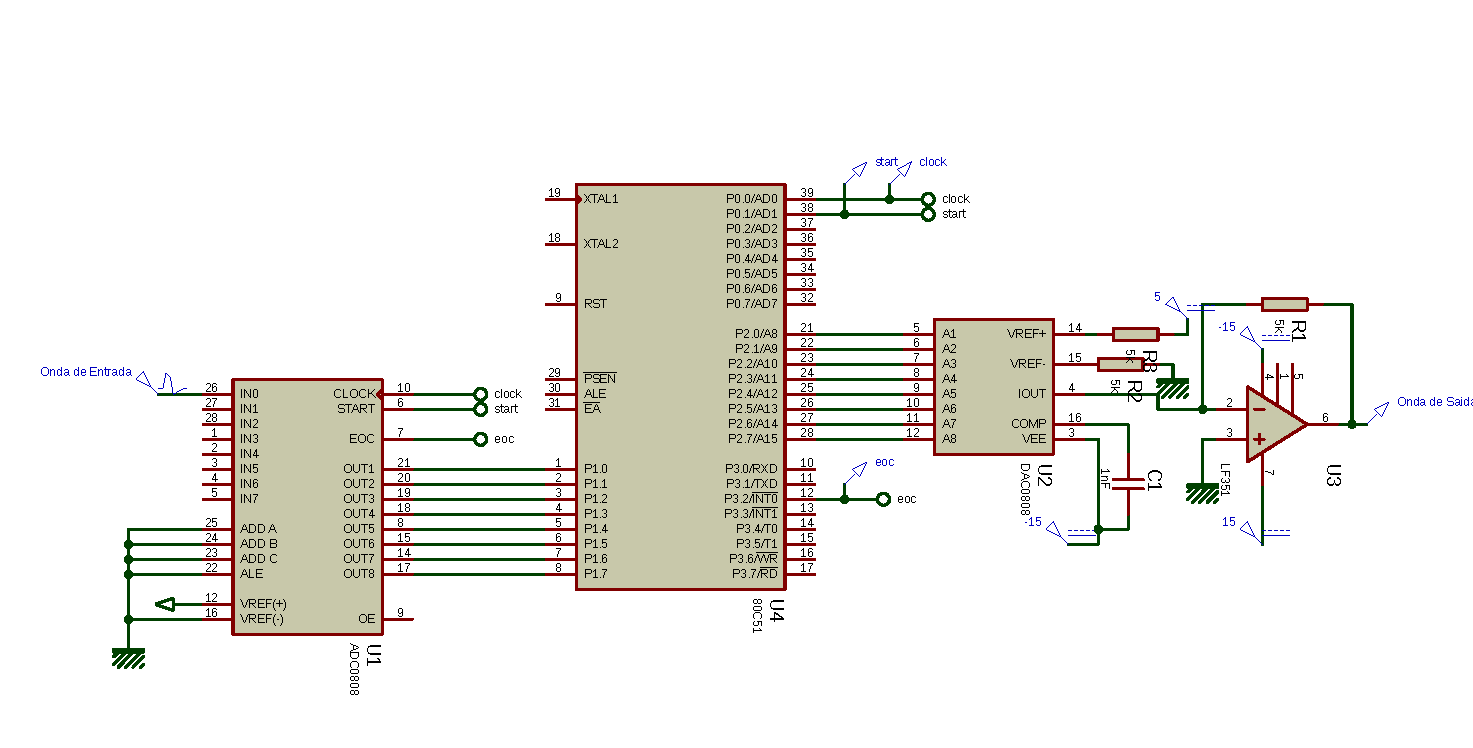
\includegraphics[width=1\linewidth]{adc_dac_completa}
		\label{fig:adc_dac_completa}
	\end{sidewaysfigure}
	%\clearpage
	%\pagenumbering{gobble}
	%\newpage
	
\begin{figure}[h!]
\centering
\includegraphics[width=1\textwidth]{adc_8051_dac.pdf}
\caption{Simulação Conversores AD DA e 80c51}
\label{fig:adc_8051_dac}
\end{figure}

\newpage

\subsection{Motor de Passo}
Uma possível aplicação de controle do 80c51 é controlando o motor de passo.Um motor de passo é um conversor eletromecânico que da uma rotação, cujo sentido e 
velocidade de rotação, dentro de certo limites, são configuráveis.Como o motor é um dispositivo que exige correntes elevadas com relação as que as portas 
do 80c51 podem oferecer, é preciso mediá-lo por meio de um driver, sendo os chips utilizados para se contruir o driver o L297 como controlador e o l298 
como dispositivo de potência.Uma leitura nos datasheet desses componentes é importante para a realização desta prática.\\
A figura (\ref{fig:motor_passo_80c51}) exprime o hardware completo com o driver do motor, lembrando que para encontrar o motor basta entrar na seleção de 
componentes e digitar motor, que surgira as opções, após isto basta escolher o stepper motor.

\begin{figure}[h!]
\centering
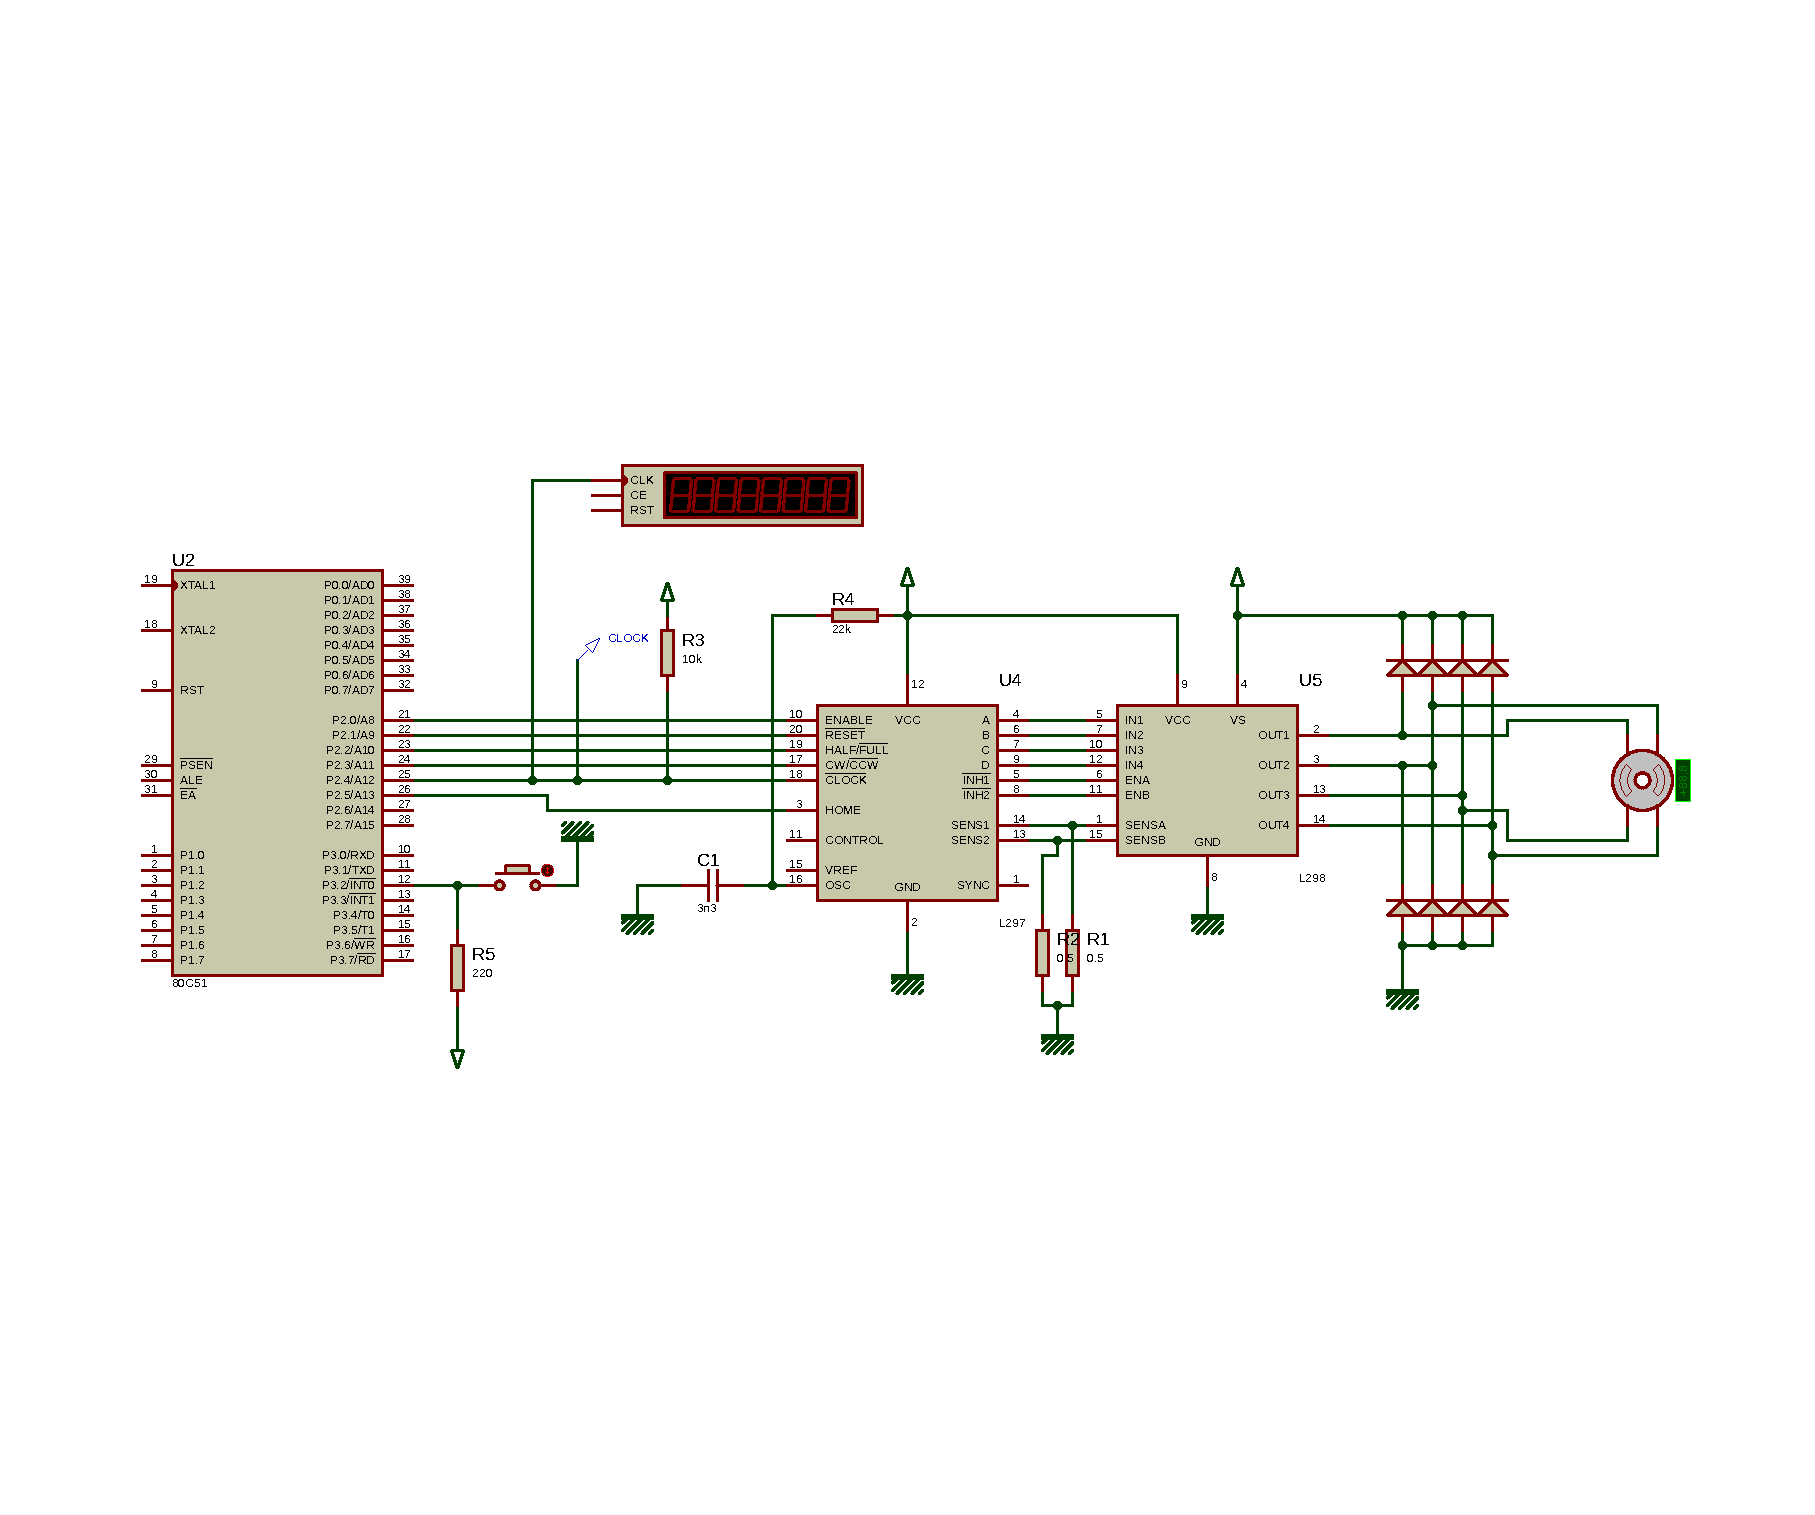
\includegraphics[width=1\textwidth]{motor_passo_80c51.pdf}
\caption{Hardware Utilizado Para a Simulação do Motor de Passo}
\label{fig:motor_passo_80c51}
\end{figure}

A simulaçao consite em fazer o motor girar para o sentido horário e esperar até que uma interrrupção externa ocorra , como isto não é possível de simular no ISIS
colocou-se o botão junto a INT0, quando pressionado o botão a interrupção é atendida e o motor espera por 5s,e gira novamente no sentido anti-horário
até haver novamente uma interrupção no mesmo pino.Após isto o motor para por dez segundos e reinicia o ciclo.\\

Esta implementação pode ser a automação de um a esteira que que para por tempos diferentes quando um objeto, ou produto, passa por um determinado sensor que
envia um sinal para o microntrolador.As paradas da esteira podem ser entendidas como tempos em o produto esteja sendo modificado.\\

Abaixo, na figura (\ref{fig:fluoxograma_motor_de_passo}), encontra-se o fluxograma que representa o código do controle do motor de passo.È preciso conhecer 
os drivers para executar a simulação, então é dito novamemte que a leitura dos datasheets é indispensável.\\

Como é necessário gerar uma onda de frequência aproximada de 10Hz para fazer com que o motor de passo se movemente, ligando o micro no driver, nos pinos 
corretos, é preciso usar a interrupção de um dos timers para realizar esta tarefa.\\

\begin{figure}[h!]
\centering
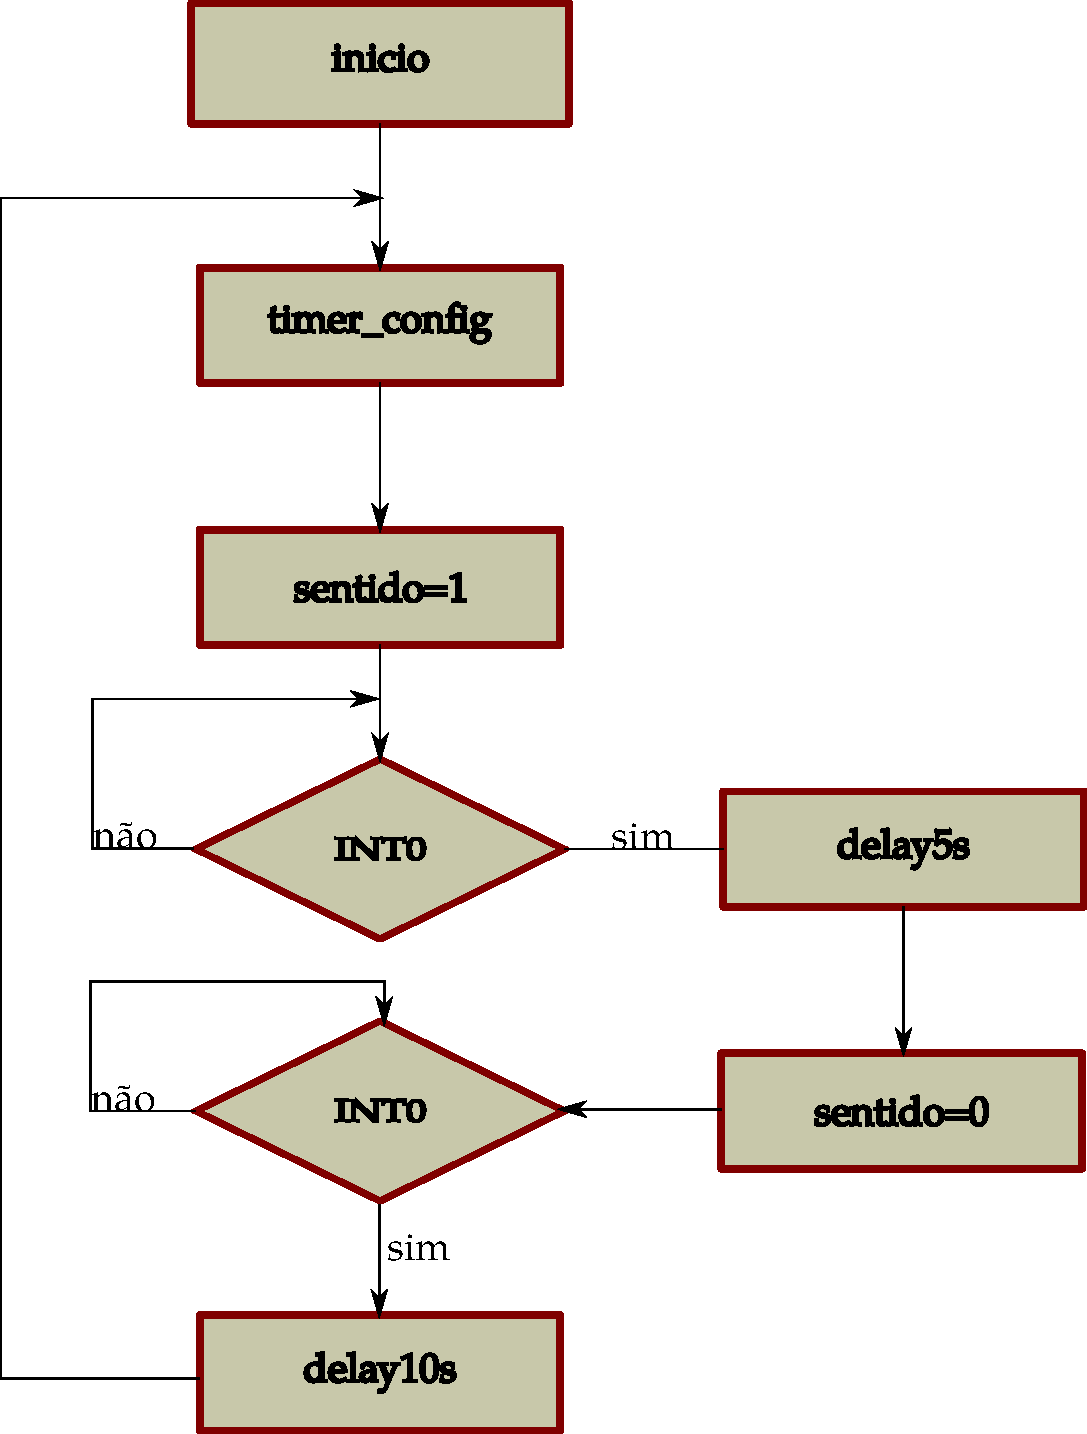
\includegraphics[width=0.5\textwidth]{fluoxograma_motor_de_passo.pdf}
\caption{Fluxograma Motor de Passo}
\label{fig:fluoxograma_motor_de_passo}
\end{figure}

\pagebreak

\subsection{Display de Sete Segmetos e LCD}
Há a disponibilidade de displays de sete segmentos para simulação animada no ISIS. Os displays devem ser multiplexados e o valor a se colocar no display
deve corresponder a conversão hexa-decimal do valor em hexa em questão.Pode-se também, simplesmente adicionar um conversor BCD a saida do microcontrolador e 
ligá-lo por sua vez aos displays.Assim basta somente multiplexá-los e colocar o valor desejado na porta aonde encontra-se o conversor.È também preciso esperar 
um tempo para o display ficar ligado com o respectivo valor.Na prática o ser humano enxerga até no máximo 30Hz, havendo um atraso que não ultrapasse essa 
frequência de acendimento de cada display, não há problemas em configurar o delay.\\

Abaixo na figura (\ref{fig:display_sete_segmetos_fluxpgrama}) encontra-se o fluxograma que traduz o codigo a ser usado para expresar um valor constante a quatro display de sete segmentos.

\begin{figure}[h!]
\centering
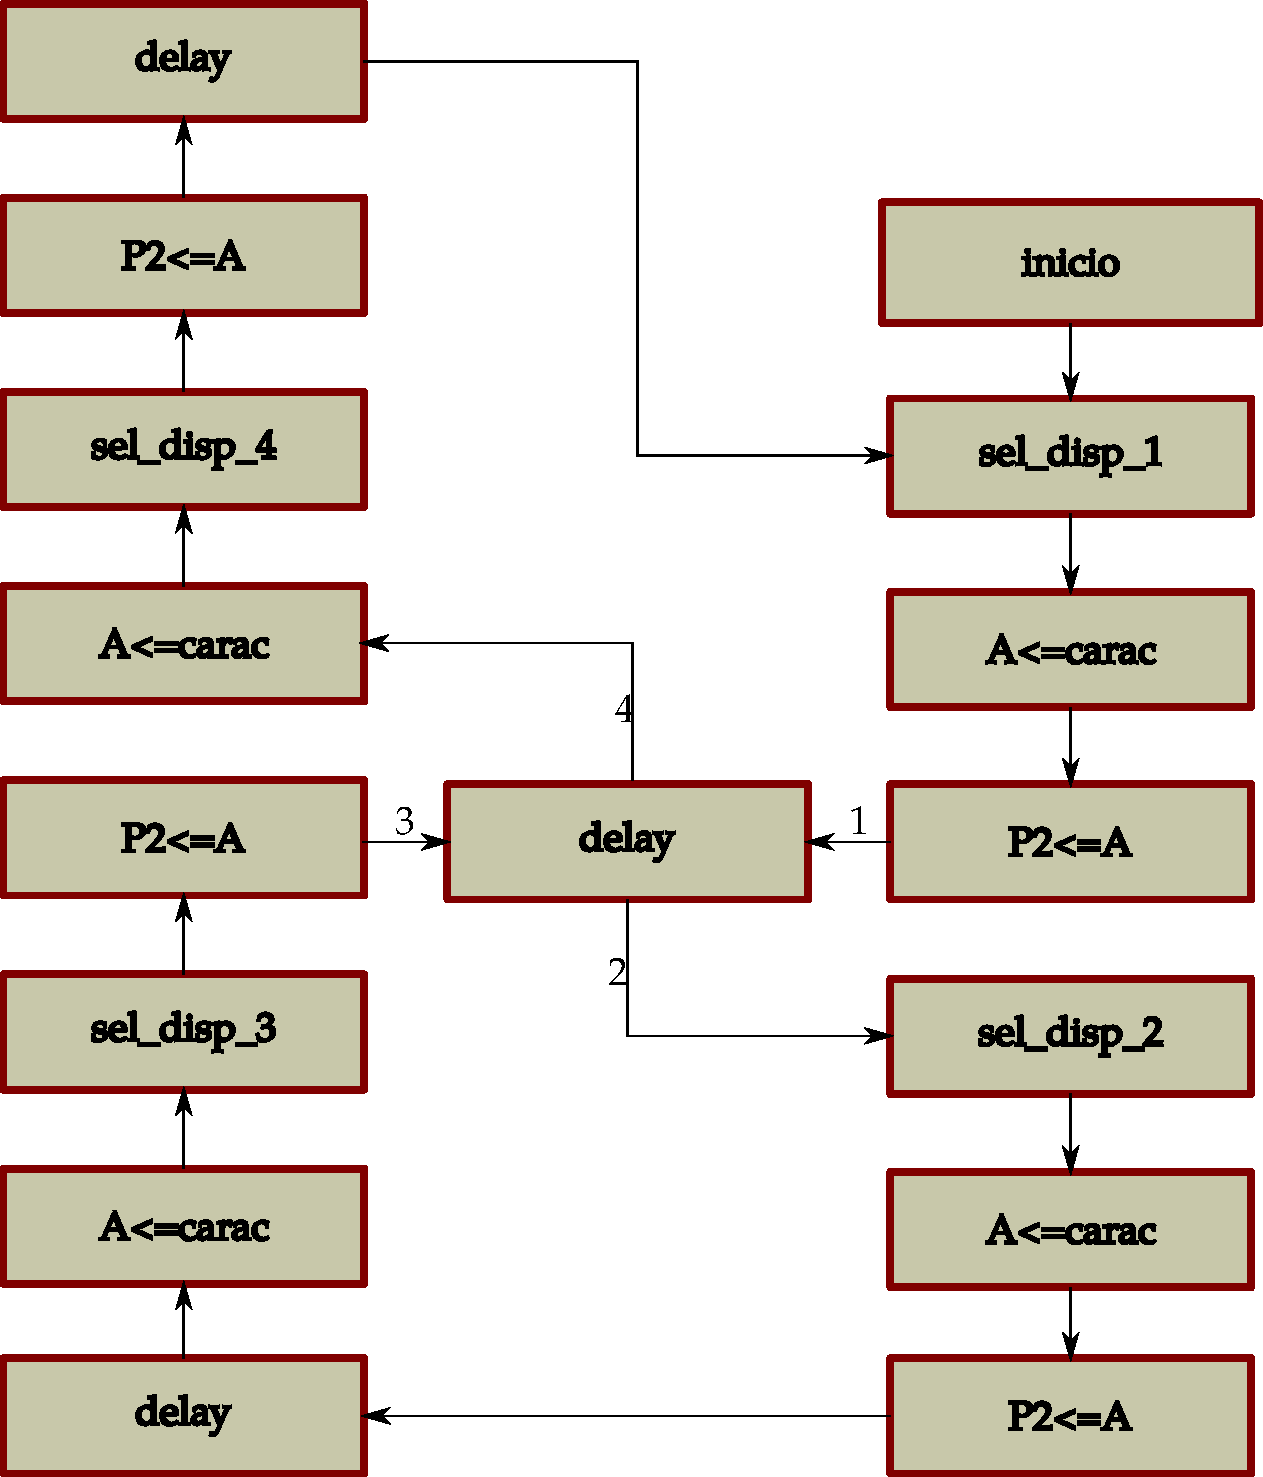
\includegraphics[width=.7\textwidth]{display_sete_segmetos_fluxpgrama.pdf}
\caption{Fluxograma Display de Sete Segmentos}
\label{fig:display_sete_segmetos_fluxpgrama}
\end{figure}

Abaixo na figura (\ref{fig:display_sete_segmentos}) encontra-se a montagem do esquemático necessario para a utilização do display de sete segmentos, considerando o uso d um conversor
BCD.

\pagebreak

\begin{figure}[h!]
\centering
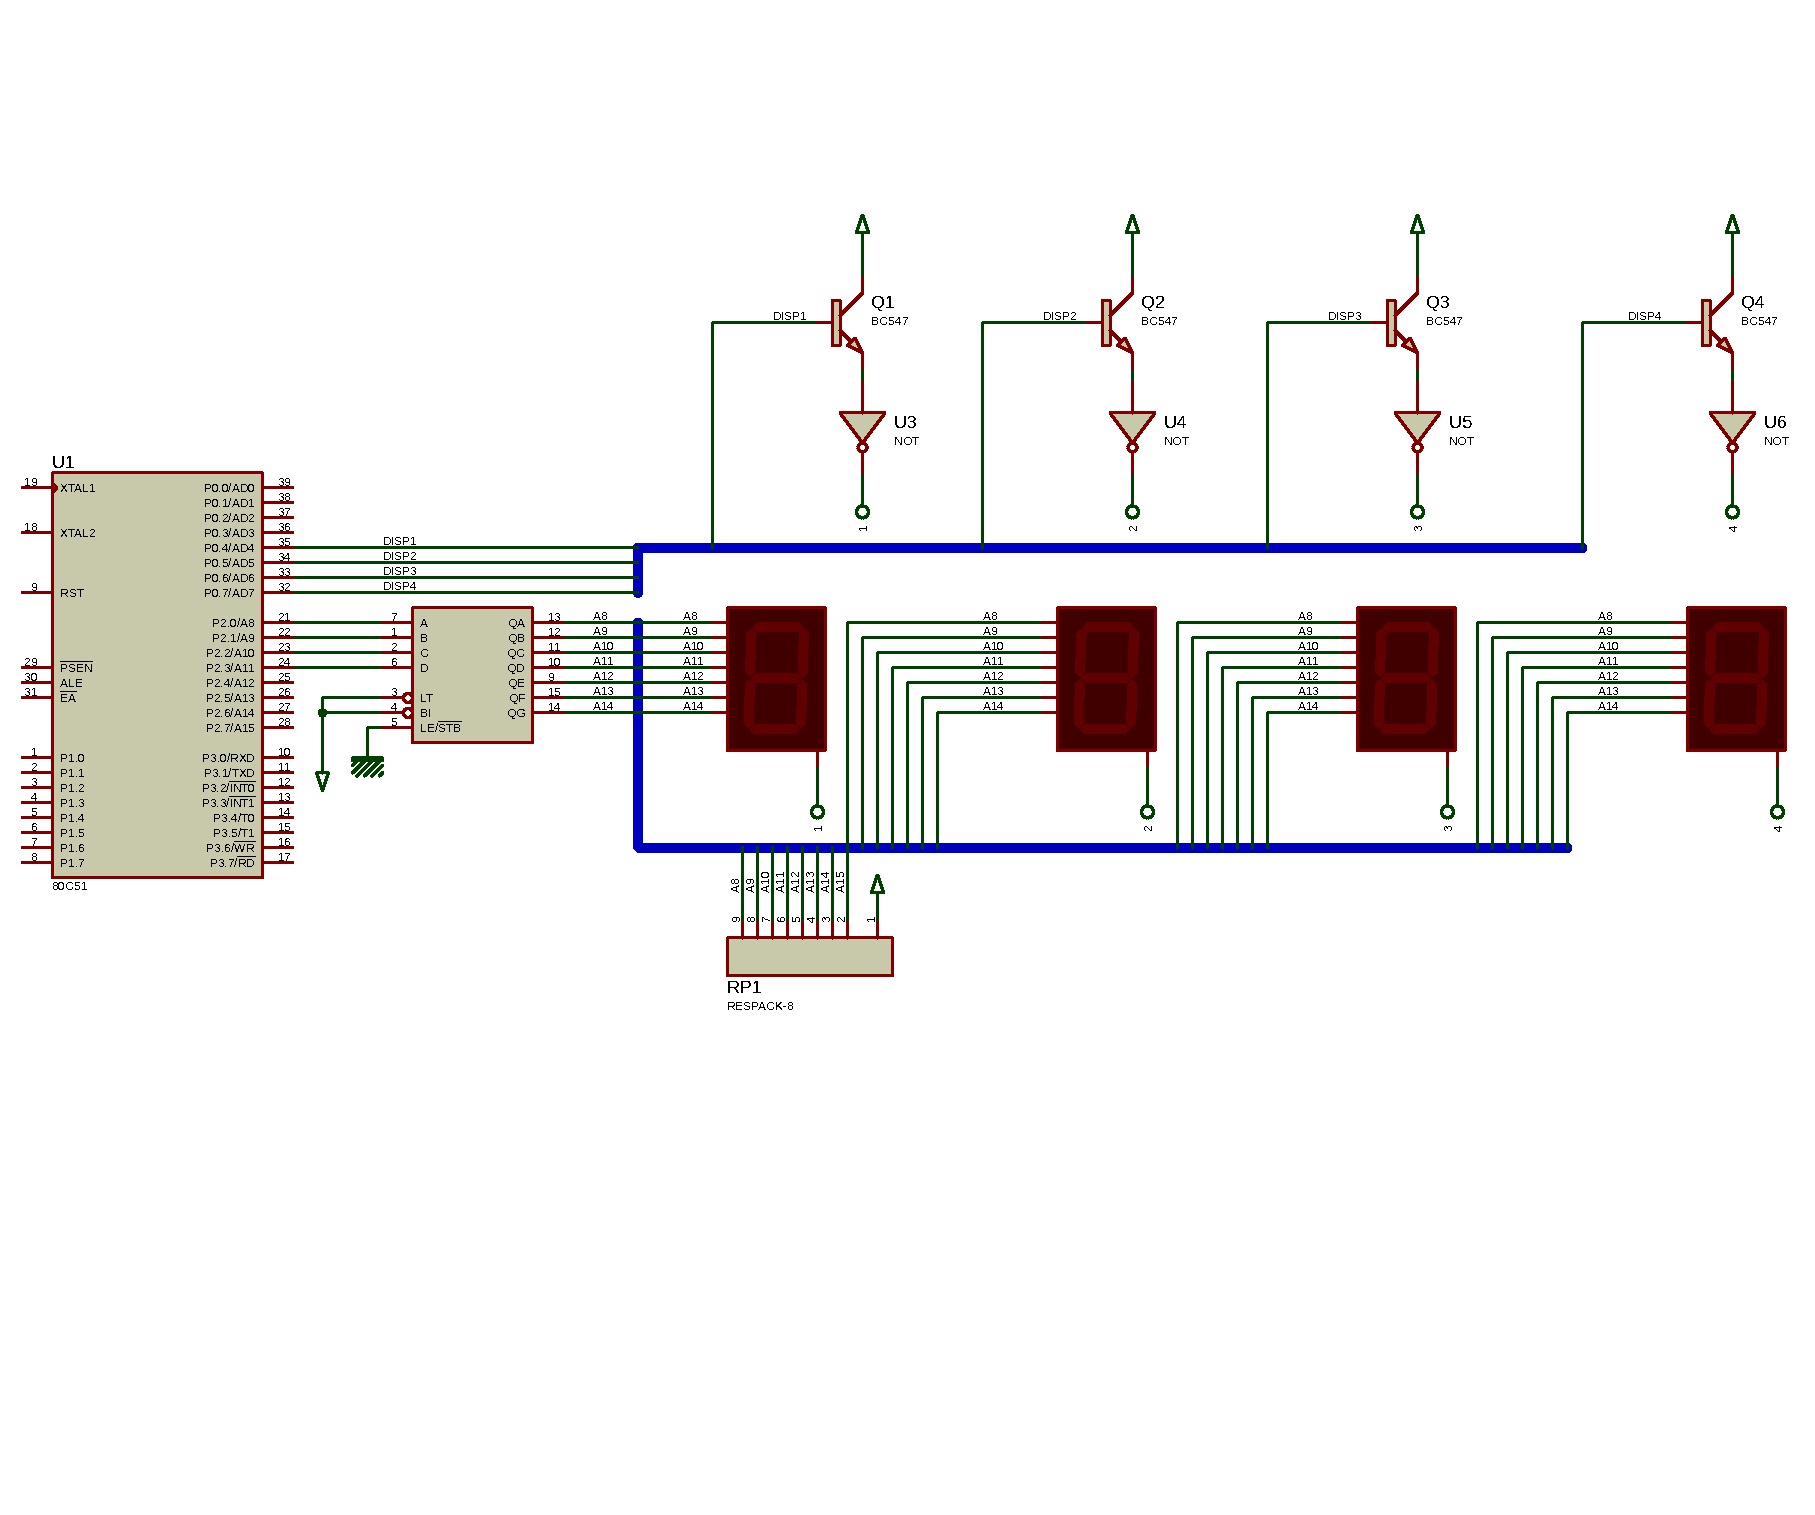
\includegraphics[width=1\textwidth]{display_sete_segmentos.pdf}
\caption{Esquemático para Simulação dos Displays de Sete Segmentos}
\label{fig:display_sete_segmentos}
\end{figure}

Para que os dispays apareçam com seus caracteres rapidamente é preciso mudar as configurações do Set Animations Options do ISIS na barra  de configurações 
opção System.Faça com que os frames da simulação apareçam mais rápido, modifique as configurações e veja o resultado.

\newpage

\subsubsection{Display LCD}
Liquid Crytal Display são largamente utilizados e fornecem um meio de interface visual com o usuário. Não raro encontra-se projetos com lcd, possibiltando 
o fornecimento de informações que estão sendo processadas para o usuário utilizá-la.\\

O uso do display exige que seja escolhida sua configuração quanto a quantos pinos serão utilizados, assim, pode-se operar tanto no modo 4 bits de dados e 
instruções quanto 8 bits de barramento.Há ainda os bits de controle E-Enable, RW-ReadWrite e RS que indica a leitura de dados ou instruções.Há disponibilidade
de vários display no ISIS, e o mais comum LM016 de duas linhas, também está na biblioteca.\\
	
É preciso ter em mente primeiramente como será a configuração do display, duas, uma linha, pixels da matriz, e enviar os dados de configuração ao display.È
importante criar uma partição que envie instruções e outra que envie caracteres ao lcd, afinal há uma diferença nos bits de controle em nivel alto e baixo
para escrever cada uma dessas informações.\\
A figura (\ref{fig:fluoxograma_lcd_crystal_liquid}) indica o fluxograma que trata como inicializar o display e escrever uma frase.

\begin{figure}[h!]
\centering
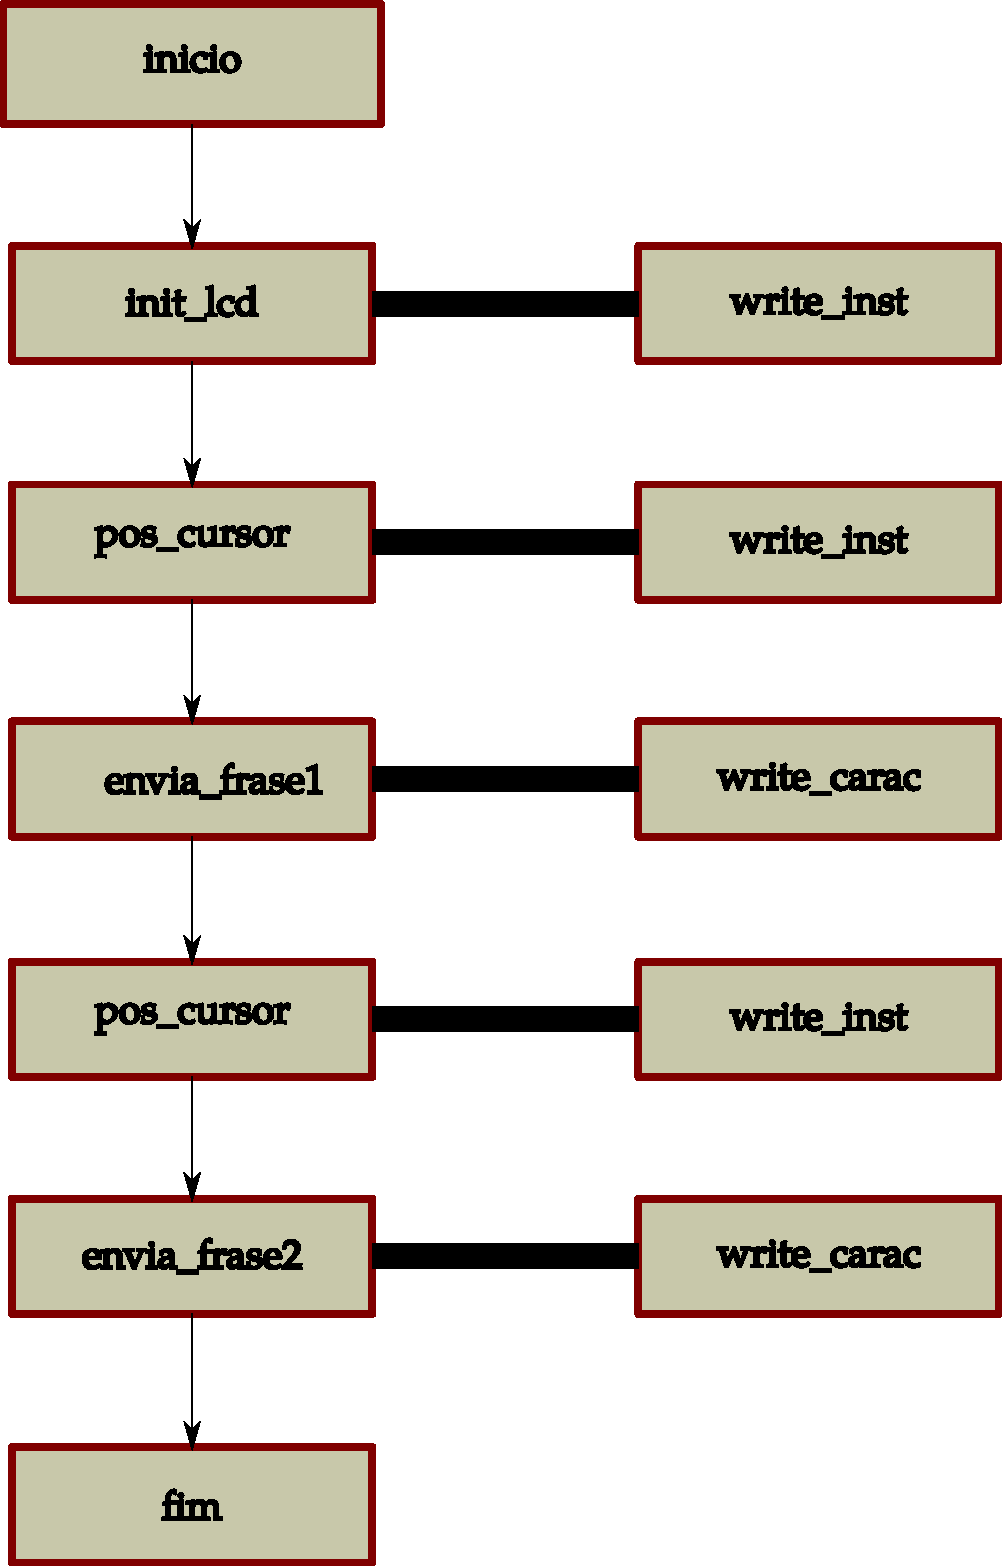
\includegraphics[width=.5\textwidth]{fluoxograma_lcd_crystal_liquid.pdf}
\caption{Fluxograma Expressando o Fundcionameto do Display LCD Tanto em 8 Como em Quantro Bits}
\label{fig:fluoxograma_lcd_crystal_liquid}
\end{figure}

\pagebreak

As duas proximas figuras (\ref{fig:lcd_4_bits}) (\ref{fig:lcd_8_bits}) ilustram o hardware já com o display em funcionamento tanto no modo 4 bits como em 8 bits.

\begin{figure}[h!]
\centering
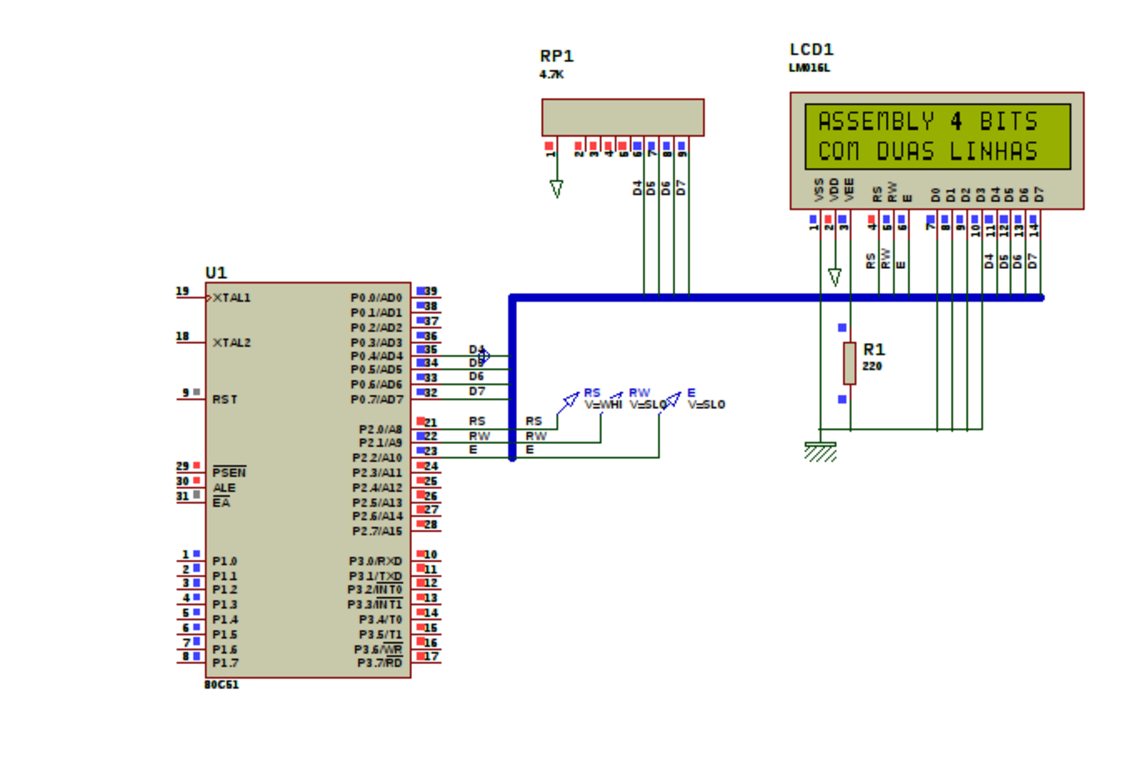
\includegraphics[width=.87\textwidth]{lcd_4_bits.pdf}
\caption{Esquemático Expressando o Funcionamento do 80c51 Junto ao LCD na Configuração 4 bits}
\label{fig:lcd_4_bits}
\end{figure}


\begin{figure}[h!]
\centering
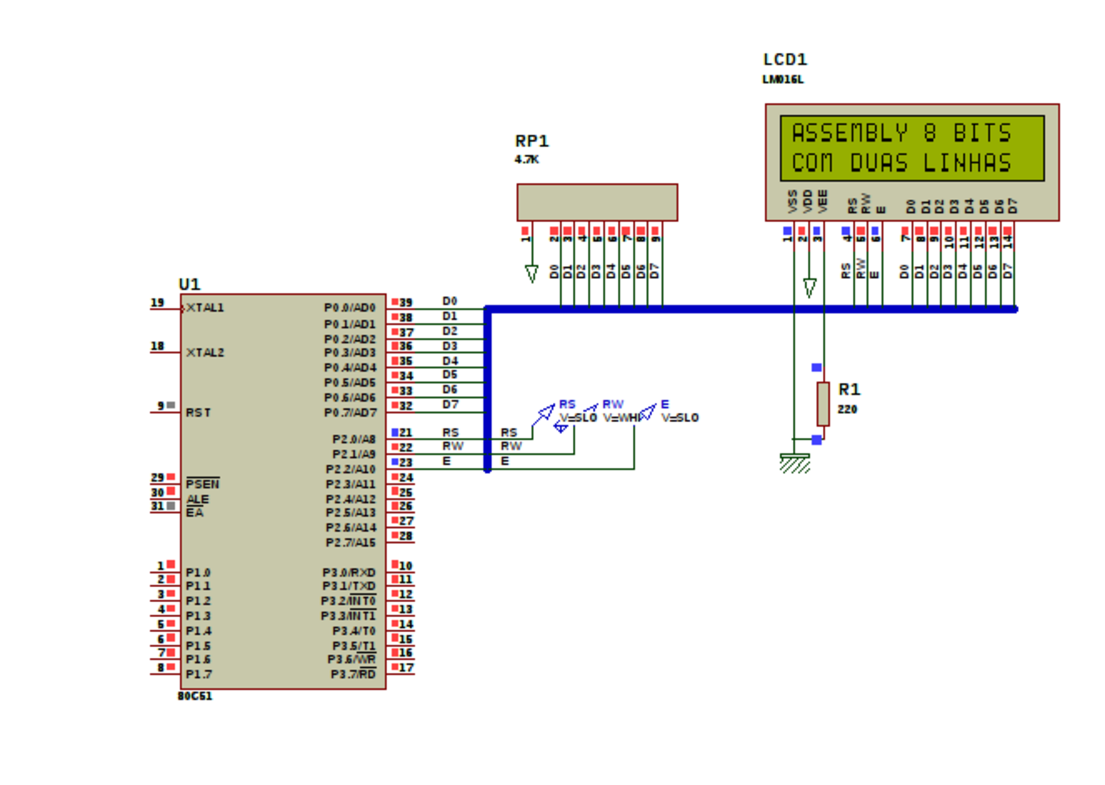
\includegraphics[width=.87\textwidth]{lcd_8_bits.pdf}
\caption{Esquemático Expressando o Funcionamento do 80c51 Junto ao LCD na Configuração 8 bits}
\label{fig:lcd_8_bits}
\end{figure}

\newpage

\section{Projetos 80c51 em Linguagem C}
Pode-se trabalhar com o microcontrolador 80c51 em linguagem C, utilizando para isto um compilador para a linguagem.Junto ao Proteus ISIS há uma janela que se
chama source code, nela é possível selecionar um compilador previamente instalado no computador e programar o micro direto do proteus, não exigindo mais que o
código deva ser carregado no micro, bastando apenas que se compile o programa e de play na execução.\\

A escolha do compilador pode ser feita antes ou depois de se construir o esquemático, podendo clicar com o botão esquerdo em cima do micro, ir em Edit Firmware
e escolher o compilador que irá usar, após isto basta programar na janela que irá abrir.\\

O compilador escolhido para a programação em C é o \textbf{SDCC}, que compila programas de alguns micrcontroladores da famila MCS80c51, incluindo o utilizado em 
todos os projetos até o momemto.\\

Para uma breve introdução em linguagem C para o 80c51, reescrever todos os programas em assembler ditados até o momento é uma boa maneira de se iniciar na linguagem aplicada ao micro.
Os projetos aqui apresentados levam em consideração que isto tenha sido feito, apresentando resultados mais rebuscados com o microcontrolador, como um frequêncimetro
, um termômetro e um modo diferente do controle do motor de passo, utilizando a interface serial.Outros projetos também encontram-se descritos.\\

\subsection{Motor de Passo Controlado Pela Interface Serial}
O hardware utilizado para a simulação do motor de passo é o mesmo apresentado na figura (\ref{fig:motor_passo_80c51}) junto aos pinos TX e RX ligados 
ao terminal serial virtual, como apresentadotado na figura (\ref{fig:serial_80c51}).\\
A simulação consiste em exibir um menu no terminal serial que possibilite ao usuário entrar com caracteres que irão identificar um possível funcionamento 
do motor de passo.As opções escolhidas estão listadas na figura (\ref{fig:terminal_serial_motor_de_passo}) que mostra o terminal com o menu escrito, 
esperando para receber um caracter e iniciar o funcionamento.\\

\begin{figure}[h!]
\centering
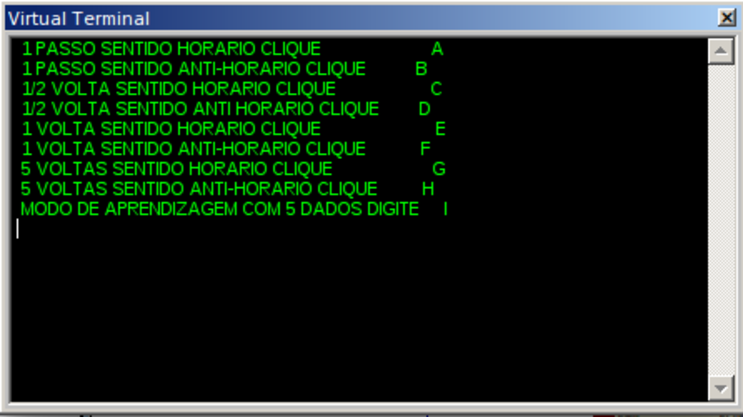
\includegraphics[width=.7\textwidth]{terminal_serial_motor_de_passo.pdf}
\caption{Terminal Serial Simulado no ISIS}
\label{fig:terminal_serial_motor_de_passo}
\end{figure}

Abaixo na figura (\ref{fig:fluoxograma_motor_de_passo_em_C}) encontra-se um fluxograma do funcionamento do programa.

\begin{figure}[h!]
\centering
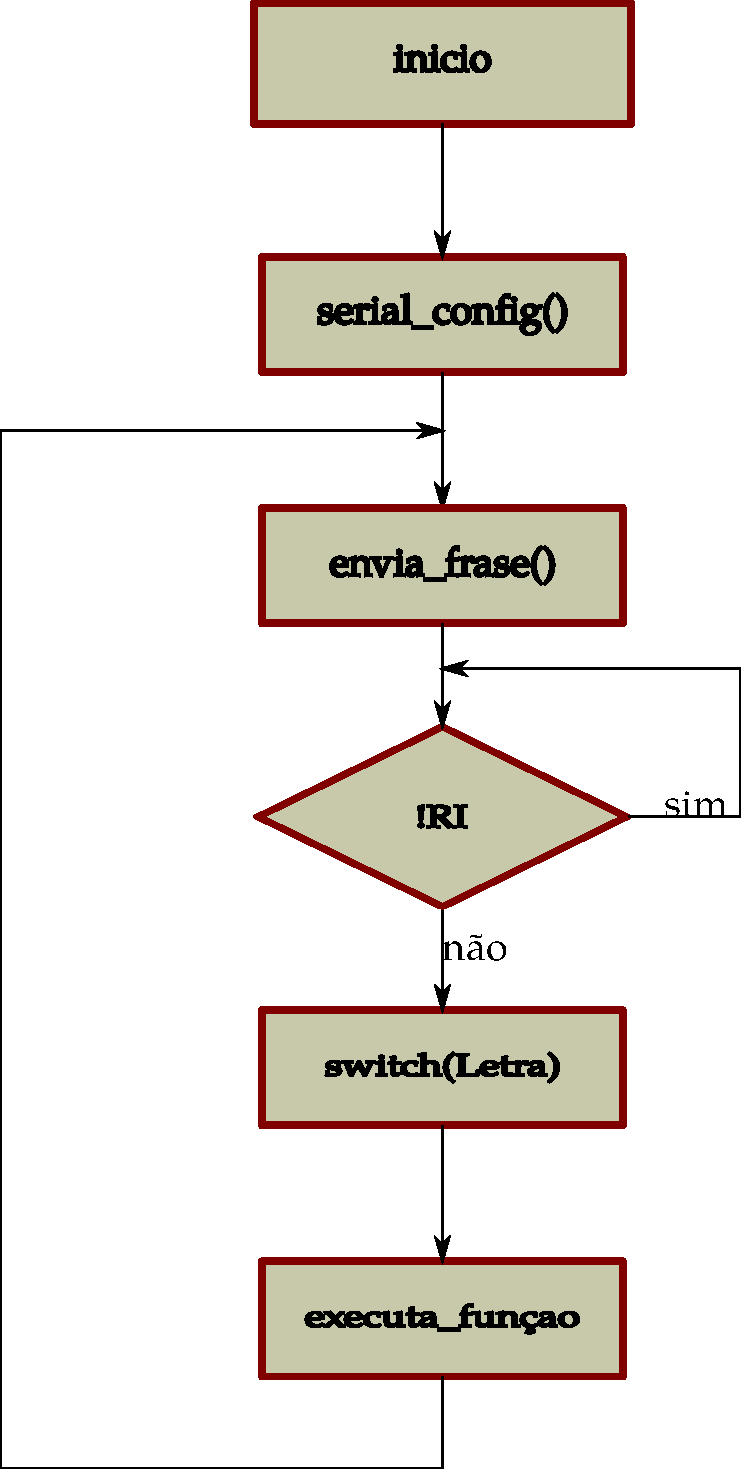
\includegraphics[width=.4\textwidth]{fluoxograma_motor_de_passo_em_C.pdf}
\caption{Fluoxograma Expressando a Construção do Porgrama do Controle Do Motor de Passo}
\label{fig:fluoxograma_motor_de_passo_em_C}
\end{figure}

A execução do programa se deu corretamente, lembrando que existe a necessidade de se ajustar o passo do motor  e saber como a informação enviada para o 
driver modificam os passos do motor, para cobrir a tarefa de girar o motor nos ângulos propostos.Foi utilizada na simulação 
10º para uma boa visualização do  giro do motor.Porém existe grande chance de não haver motores com este passo no mercado.Assim, antes de simular, verifique, caso 
tenha interesse na realização do projeto, o passo do motor real e colocar nas configurações do proteus,bastando clicar sobre o motor e configurar o passo do mesmo.\\
Outras opções para o motor também estão disponíveis.

\pagebreak

\subsection{Frequêncimetro}
É possível implmentar um frequêncimetro com o 80c51, utilizando o fato de que o mesmo possui um contador de pulsos e permite programar um delay, 
seja via timer ou atraso.\\
Asssim basta deixá-lo contando por um segundo e exibir o valor da contagem. Encontra-se o fato de que o contador é de dezesseis bits, 
havendo a necessidade de se converter o numero para decimal, fazendo assim a operação de trabalhar com dois registradores, DPH e DPL, traduzindo-os em um 
só número.O projeto fica completo quando adiciona-se um display que exibe a frequência medida.Como já sabemos  o programa do lcd, basta utilizá-lo em conjunto 
com o main.c do frequêncimetro, possibilitando o uso de funções do lcd.\\
O fluxograma que exibe o comportamento do programa que controla o sistema encontrase na figura (\ref{fig:fluxograma_frequencimetro}).\\

\begin{figure}[h!]
\centering
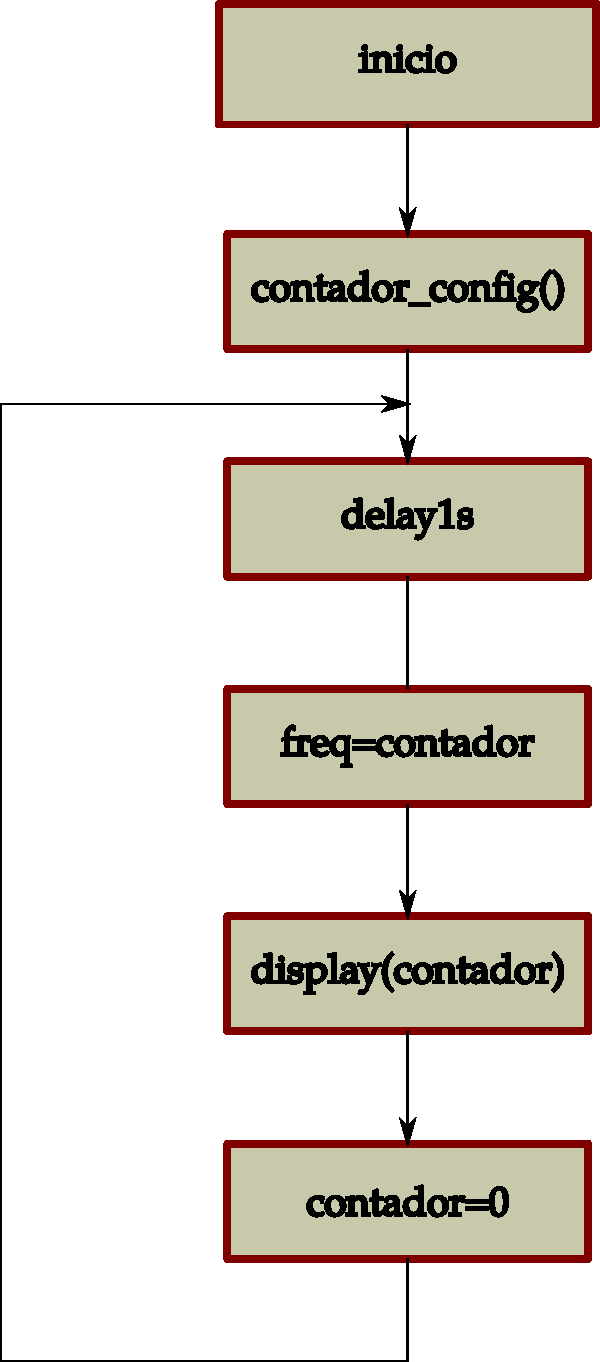
\includegraphics[width=.3\textwidth]{fluxograma_frequencimetro.pdf}
\caption{Fluoxograma Expressando a Construção do Porgrama do Frequêncimetro}
\label{fig:fluxograma_frequencimetro}
\end{figure}

O funcionamento do programa se deu corretamente com poucos porcento de erro.Lembrando que o micro é capaz de medir no minimo 1 Hz e no máximo a metade de frequência 
do osciloador do micro.\\
Abaixo na figura (\ref{fig:frequencimetro_display}) encontra-se o display com uma interessante ferramenta que é a de seleção de esqueático.Selecionando oque você deseja 
ver durante a simulação animada após isso bastando somente cliar em mensagem durante a simulação, com isto irá aprecer somente os itens selecionados.
Verifica-se que a frequência exibida no display é de 537Hz enquanto a de entrada
é no valor de 535Hz, havendo boa precisão na contagem.\\
O hardware é apenas o visto para ligar o display, seja no modo 8 bits ou 4 colocando um gerador de onda quadrada no pino do contador, que é T0 ou T1.

\begin{figure}[h!]
\centering
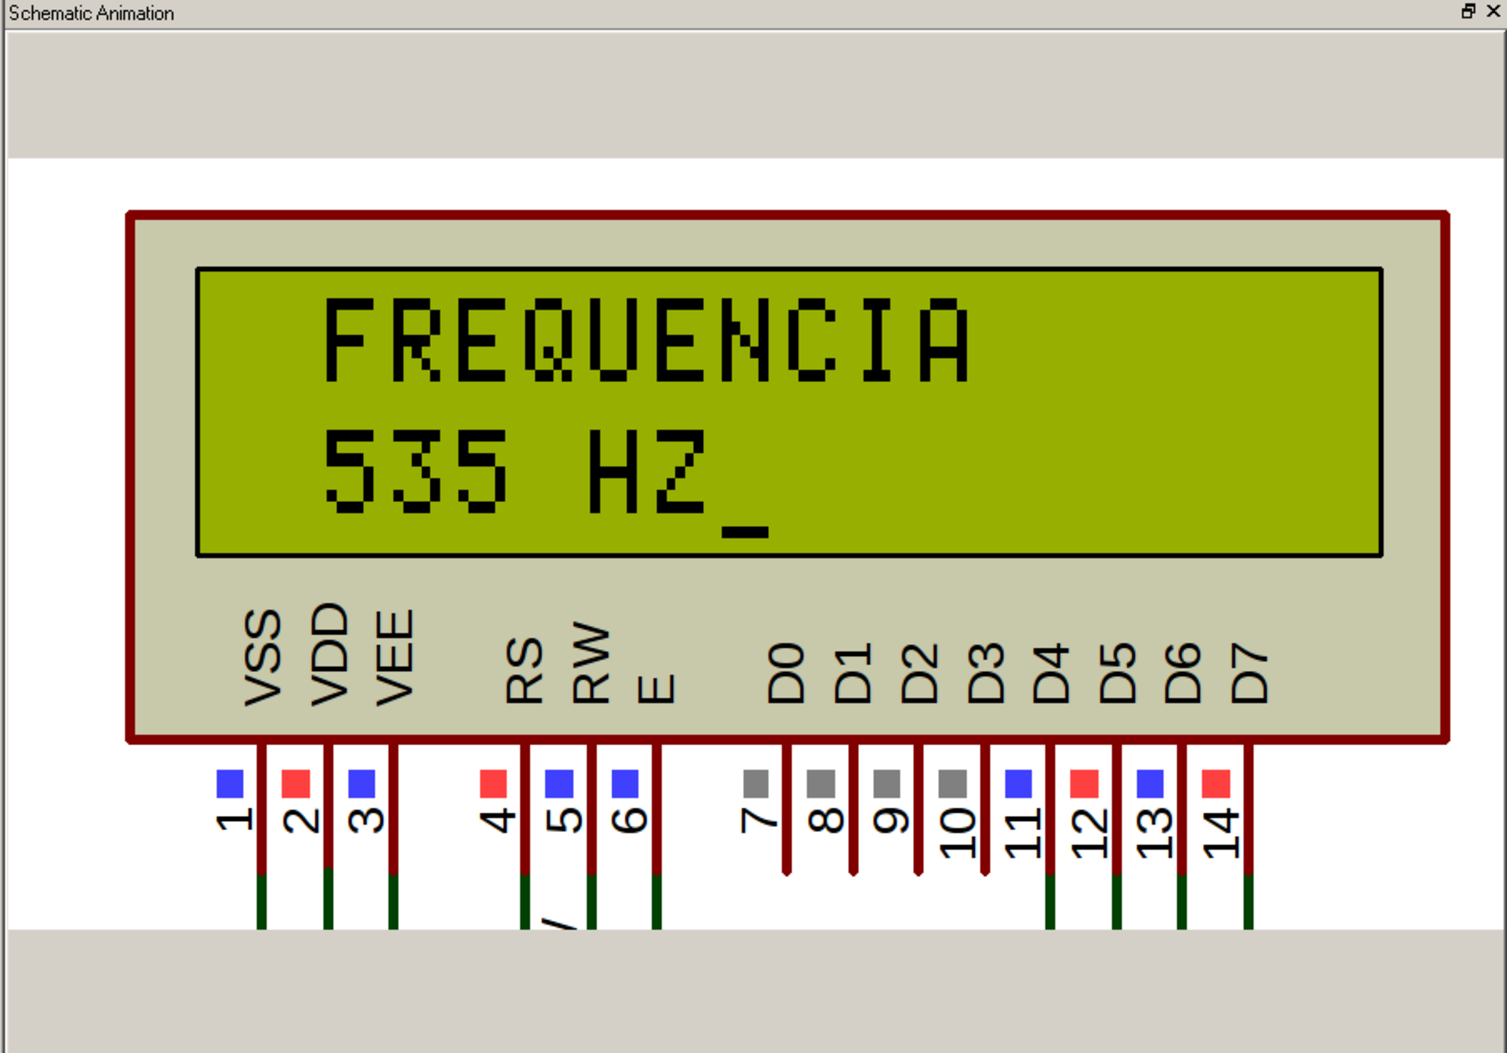
\includegraphics[width=.6\textwidth]{frequencimetro_display.pdf}
\caption{Valor Mostrado no Display Qando a Entrada é 535Hz}
\label{fig:frequencimetro_display}
\end{figure}


\newpage

\subsection{Termômetro com Tabela e Polinômio}
A conversão digital analógica permite processamento ou tabelamento de dados digitalizados, permitindo  que se faça uma relação entre o digitalizado e uma informação, 
que no presente caso, refereçe-se a temperatura que o sinal analógico esta indicando.\\

Como já foi comentado a respetio da programação do conversor AD e sua configuração basta dizer que o processo de contruir um termômetro é construir um vetor de  char, 
sendo cada char a temperatura do valor lido no conversor AD.Desta forma tem-se a seguinte configuração do programa, expressa no fluxograma da figura (\ref{fig:fluxograma_termometro_tabela}) abaixo.

\begin{figure}[h!]
\centering
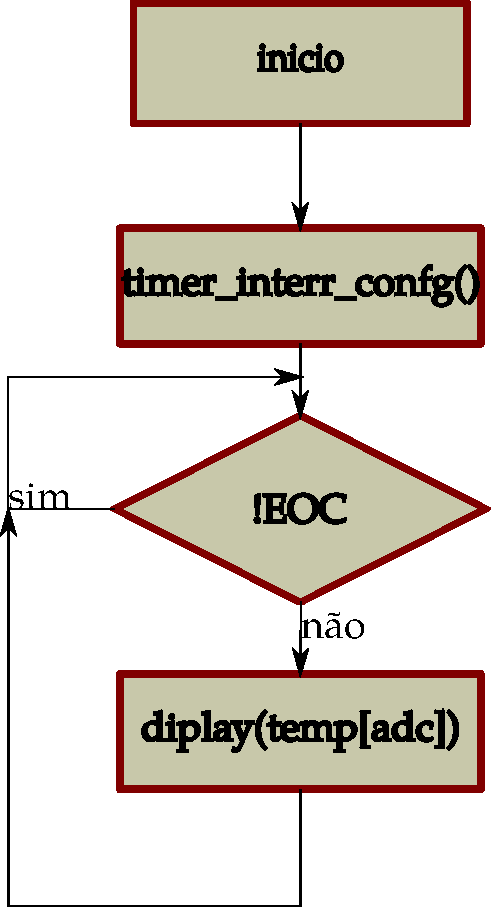
\includegraphics[width=.3\textwidth]{fluxograma_termometro_tabela.pdf}
\caption{Fluoxograma Expressando a Construção do Porgrama do Controle Do Termômetro por Tabela}
\label{fig:fluxograma_termometro_tabela}
\end{figure}

Para o programa em questão foi montada uma tabela que ia de -15ºC a +15ºC, para valores de 00h no converor a 1fh, dai para cima mostra limite superior no display.\\
Para fazer modificações basta moficar os valores na tabela de acordo com o endereço especificado pelo conversor AD.\\
Abaixo na figura (\ref{fig:hardware_termometro}) encontra-se o hardware utilizado para realizar a simulação bem como o resultado dado nos diaplay,
expresso na figura (\ref{fig:display_termometro_tabela}).
O termomêtro pode ser construído partir de um polinômio que recebe o valor DA convertido processa-o e entrega o valor da temperatuda relacionada.Quanto ao fluxograma 
de projeto muda somente o fato de que o display imprime a o valor \textbf{polinômio(adc)}.

\begin{figure}[h!]
\centering
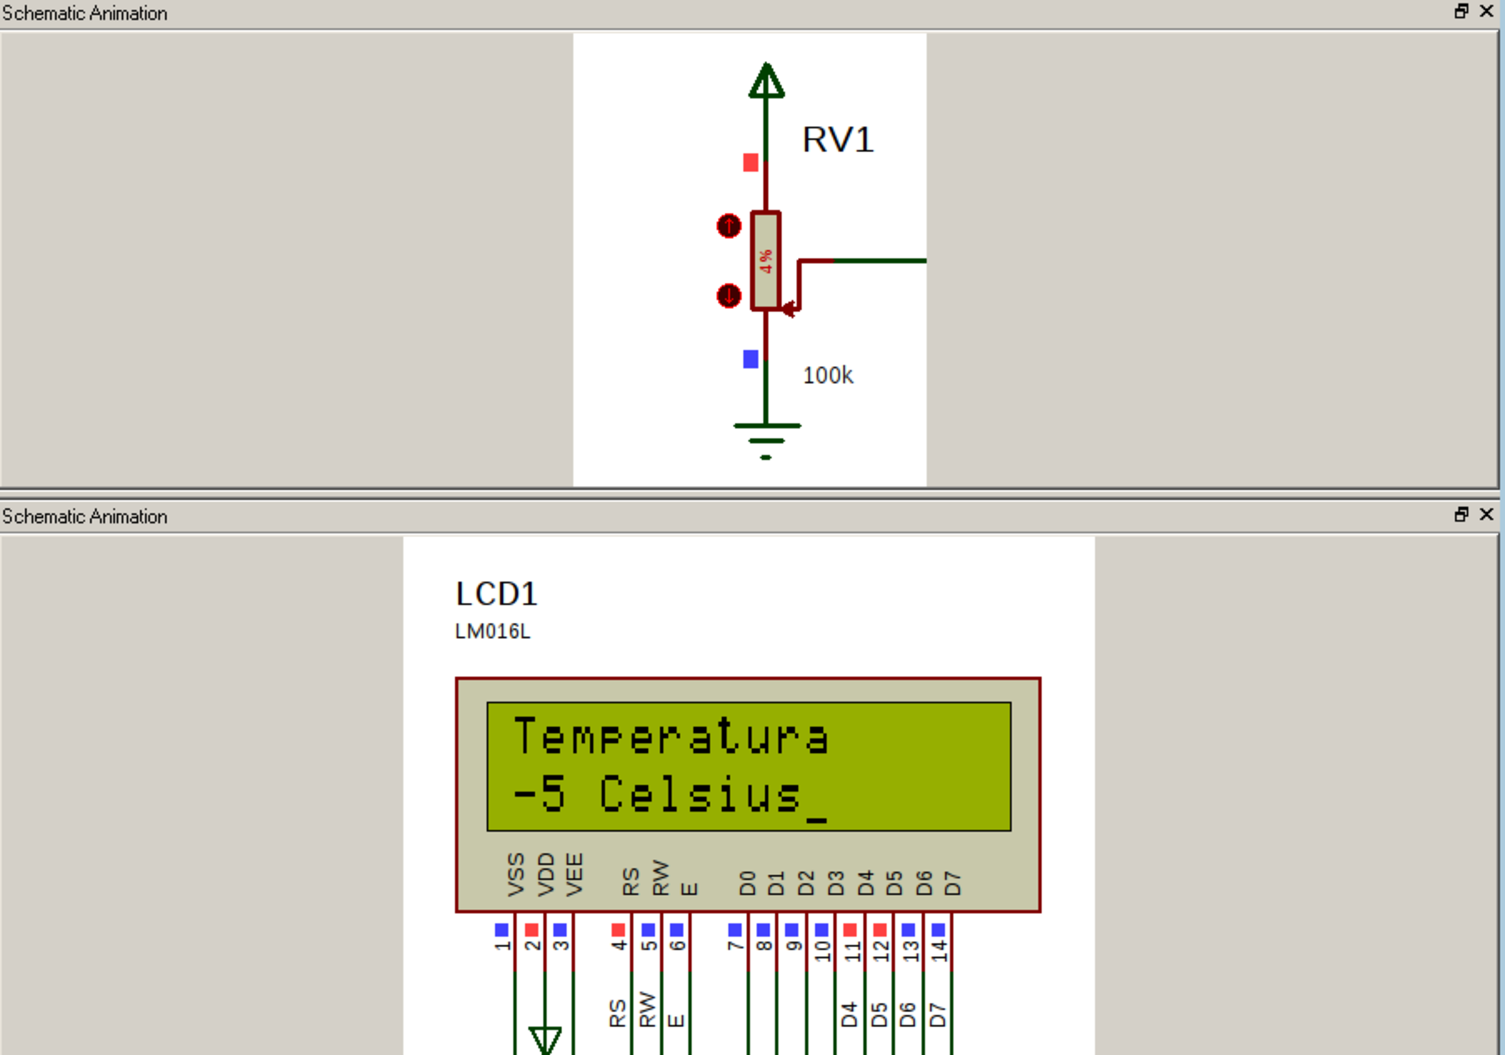
\includegraphics[width=0.7\textwidth]{display_termometro_tabela.pdf}
\caption{Valor Mostrado No Display Quando o Micro é Programado Como sendo um Termômetro por Tabela.}
\label{fig:display_termometro_tabela}
\end{figure}
	
	\newpage
	%\thispagestyle{empty}
	\clearpage
	\begin{sidewaysfigure}[h!]
		\centering
		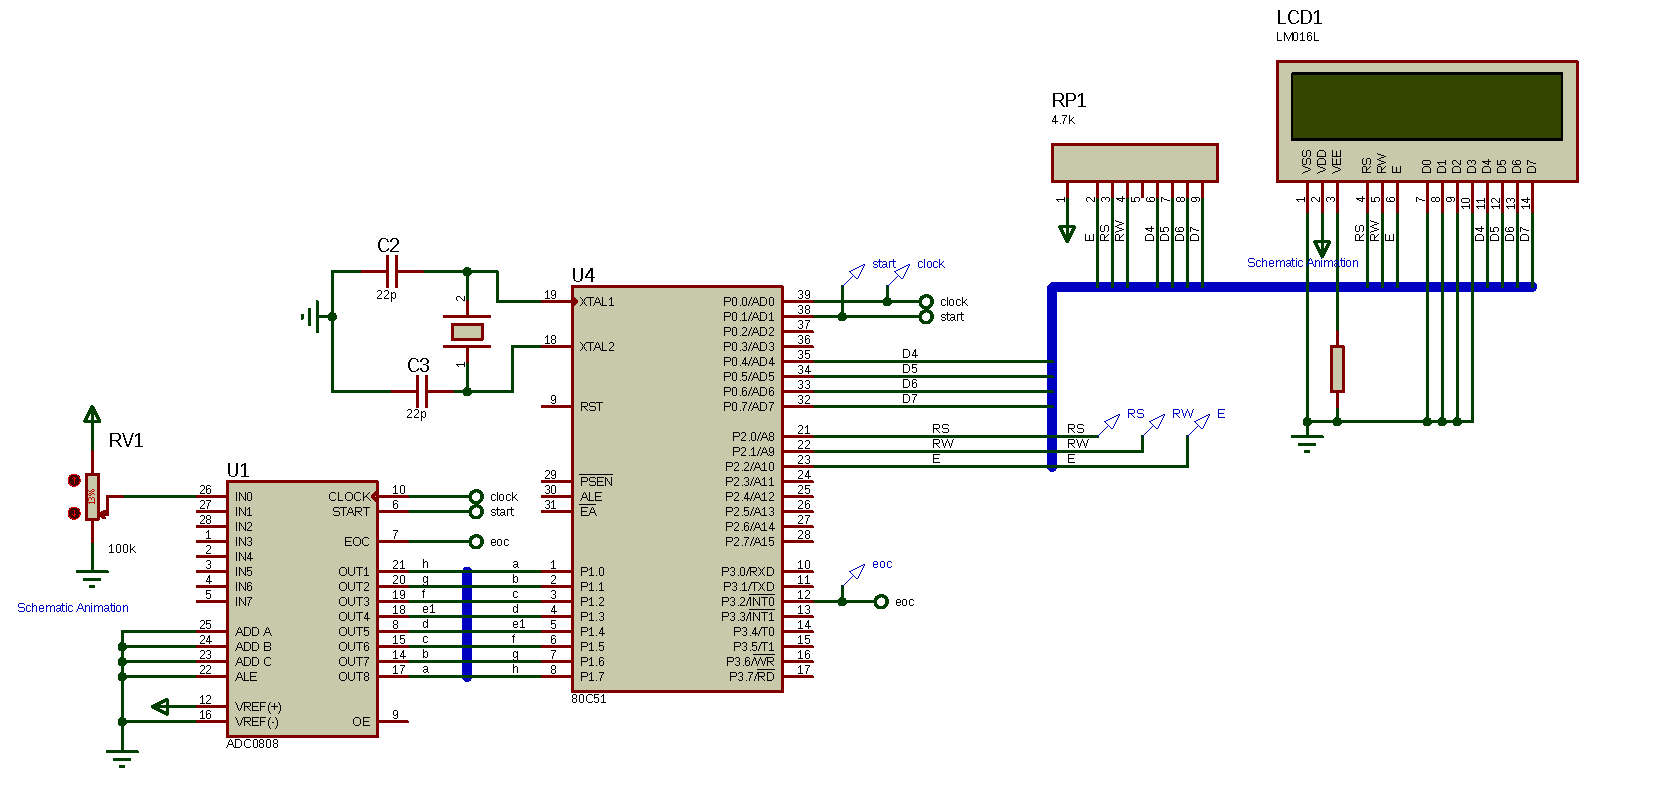
\includegraphics[width=1\linewidth]{hardware_termometro}
		\label{fig:hardware_termometro}
	\end{sidewaysfigure}
	\clearpage
	%\pagenumbering{gobble}
	\newpage
	

\section{Projeto de Dipositivos Decodificados}
Como vem sido expresso neste trabalho, é muito importante ligar varios dutos da porta P0 do micro de deocdifucá-la, permitindo
assim o uso de varios dispositivos pelo microcontrolador.\\
Levando em consideração a prática dessa estrutura o projeto seguinte consiste em montar um circuito com o 80c51  que conteha os itens baixo,
e simulá-los para verificar seu funcionamento.\\

\begin{itemize}
 \item Memória de prograna externa mínima de 8k
 \item Memória de dados expterna mínima de 8k
 \item Teclado Matricial de 16 Caracteres
 \item Quatro Motores de Passo com Acionamento Independentes
 \item Um Sensor Óptico Conectado a Entrada T0
 \item Um Conversor AD de 8 Bits
 \item Um conversor DA de 8 Bits
 \item Interface Serial de 8 Bits
\end{itemize}

	\newpage
	%\thispagestyle{empty}
	\clearpage
	\begin{sidewaysfigure}
		\centering
		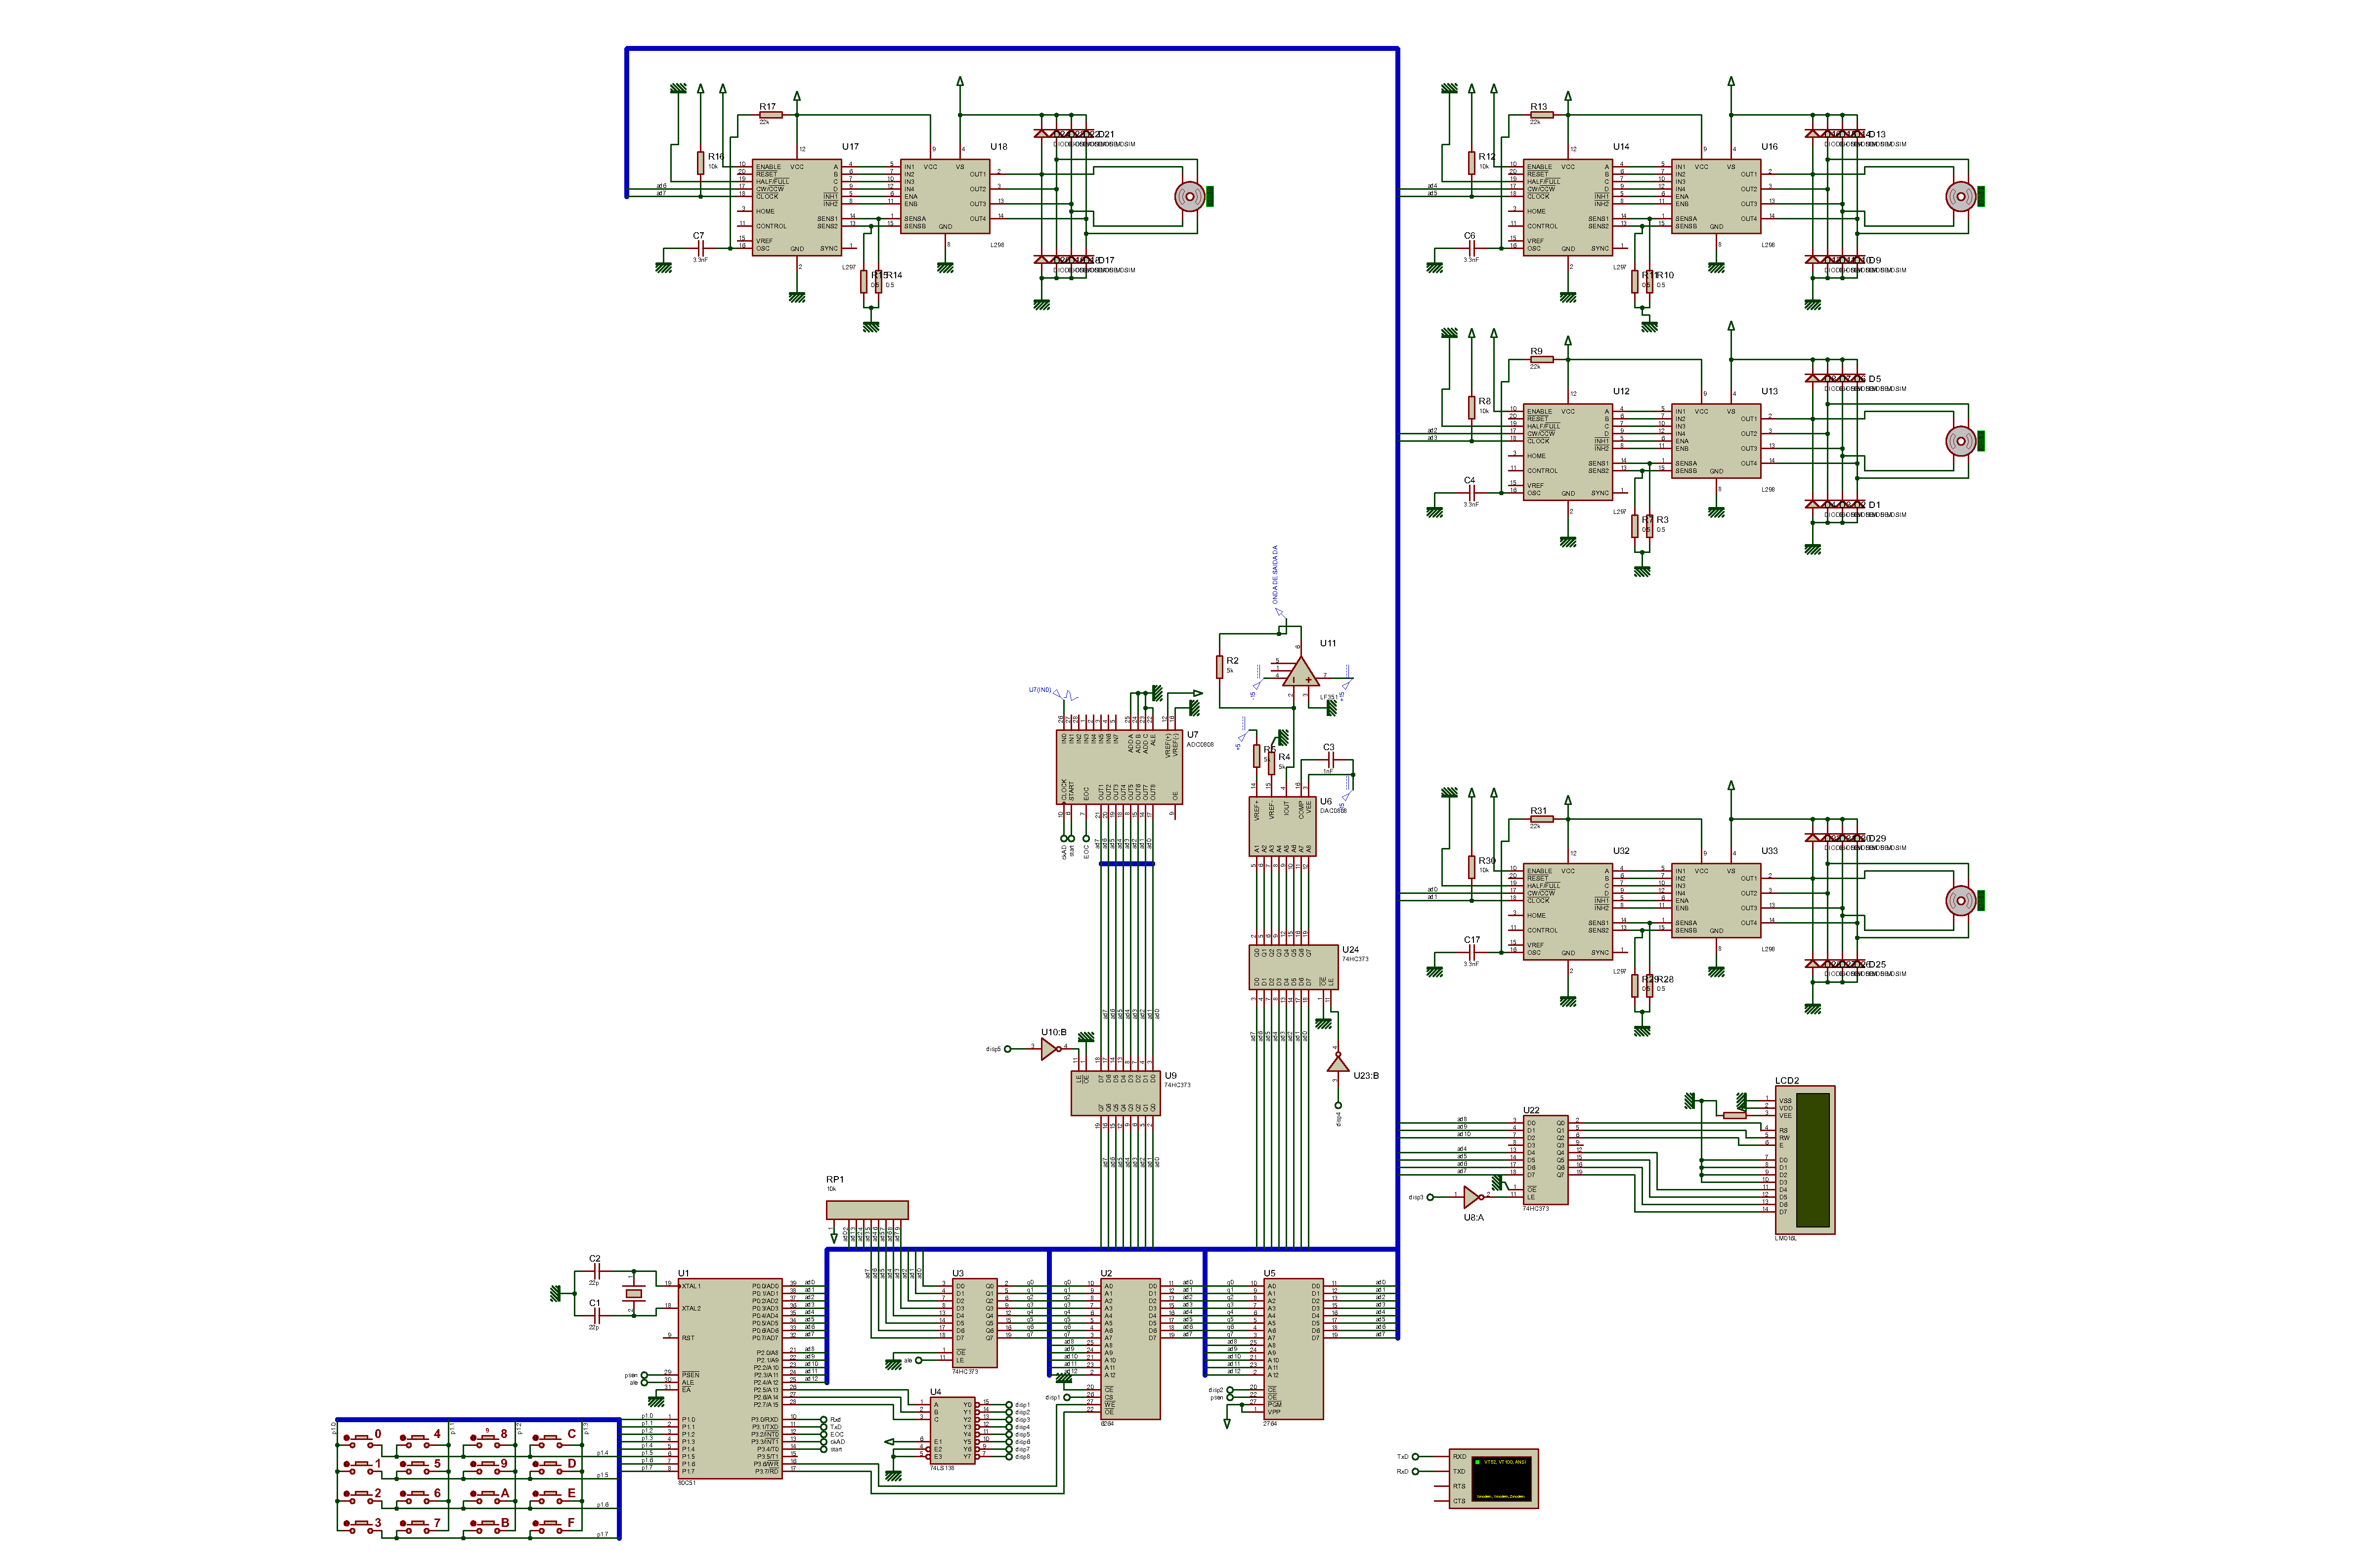
\includegraphics[width=1\linewidth]{projeto_final.pdf}
		\label{fig:projeto_final}
	\end{sidewaysfigure}
	\clearpage
	%\pagenumbering{gobble}
	\newpage

Como pode ser visto pelo esquemático, apresentando na figura (\ref{fig:projeto_final}) o mesmo constitue-se de elementos todos estudados nos demais tópicos do 
projeto total, podendo ser simulado utilizando qualquer um dos
códigos feitos, porém fazendo previa decodificação do elementou ou utilizar o endereçamento pelo registrador DPTR, sendo que cada elemento do decodificador,
seleciona o dispositivo desejado.Cada passo entre um e outro dispositivo do decodificado possui uma faixa de 1fffh.\\
Portanto tem-se:\\
0000h--1fffh  disp1\\
2000h--3fffh  disp2\\
4000h--5fffh  disp3\\
6000h--7fffh  disp4\\
8000h--9fffh  disp5\\
a000h--bfffh  disp6\\
c000h--dfffh  disp7\\
e000h--ffffh  disp8\\
Outro modo é usar a função MOVC A, @A+DPTR com o DPTR direcionando para o endereço que irá selecionar o referido dispositivo a que se deseja trasmtir ou 
receber um dado.

\section{Conclusões}
No que diz respieto a simulação de circuitos digitais, principalmente a utilização do microcontrolador 80c51, foi dado uma abordagem inicial de como utilizar o
sistema PROTEUS ISIS para simular os elementos consituintes do circuito.Lembrando que a gama de microntroladores disponíveis no ISIS é gigante, sendo que, o
objetivo deste relatório é introduzir o usuário ao simulador, deixando a ele novas aventuras, como o aprendizado de novos microcontroladores mais usados no 
mercado, como PIC's, microcontroladore atmega, base da plataforma arduino.Abaixo, na figura (\ref{fig:8_bits_pretencao_de_uso_microcontroladores}), 
encontra-se um gráfico falando sobre qual microcontrolador de 8 bits é provável de se usar no próximo projeto em questão, aonde vê-se que não há pretenção 
no uso do 80c51.Assim, aprendendo somente o 80c51 é ter apenas uma base de microcontroladores.O softtware Proteus ISIS  possibilita o aprendiizado de 
novos micros mais usados. Caso tehna sido feita todas as simulaçãoes presentes no projeto, o aluno terá uma boa experiência com simulações no proteus, havendo
apenas a necessidade de se transitar para um novo microcontrolador, ou seja, uma nova aquitetura e compilador, crucial para dar  caminho a 
sua jornada junto a outro microcontroladores.

\begin{figure}[h!]
\centering
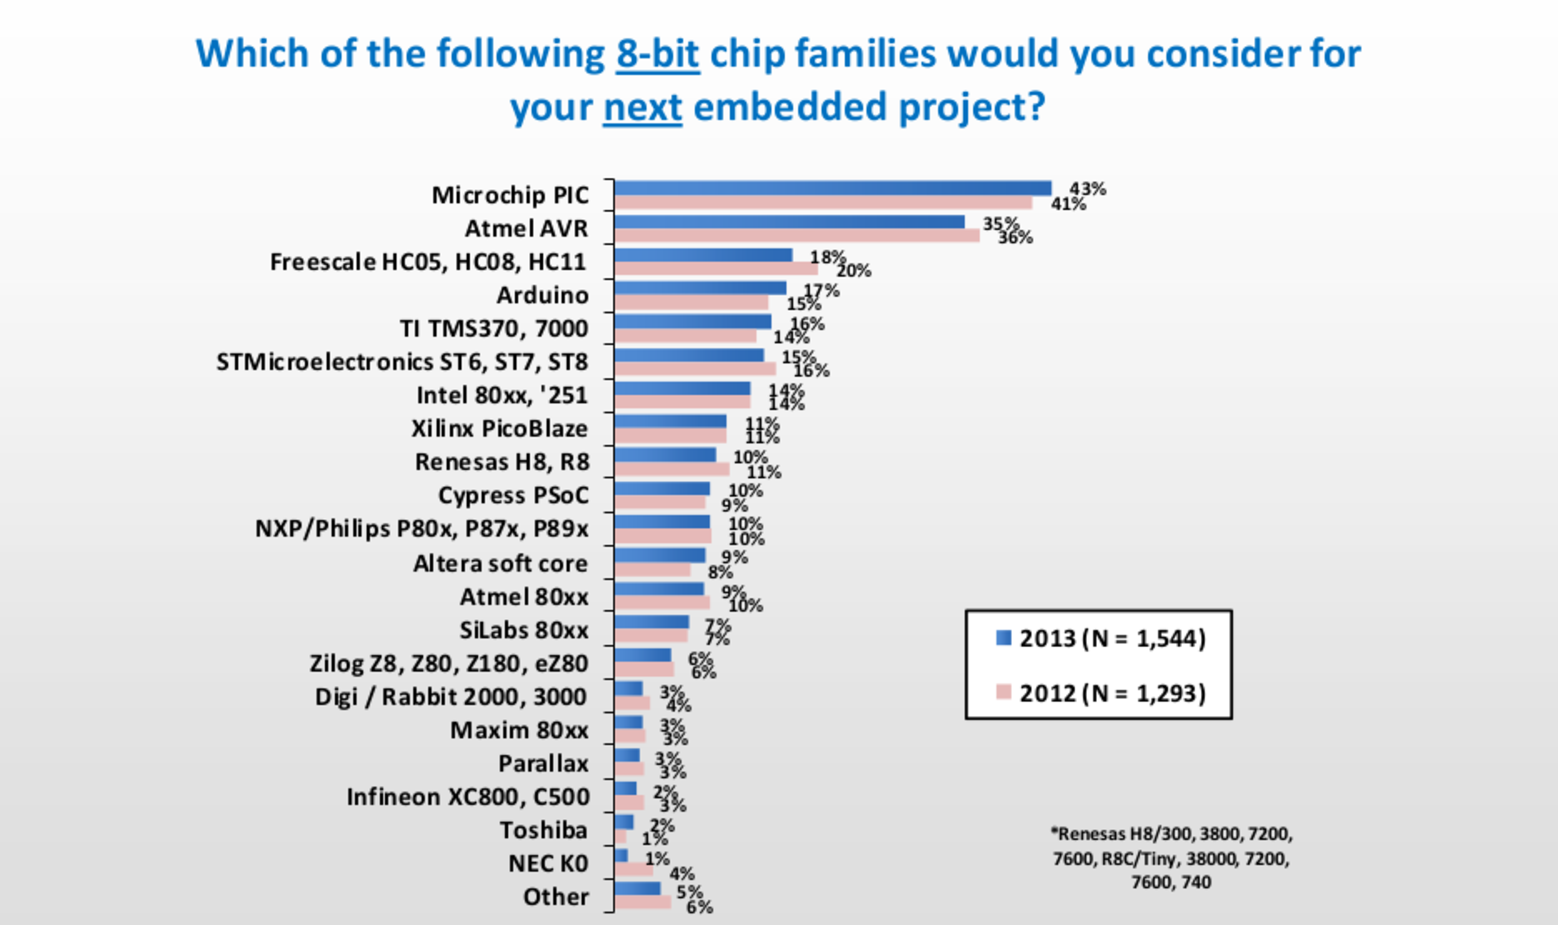
\includegraphics[width=.7\textwidth]{8_bits_pretencao_de_uso_microcontroladores.pdf}
\caption{Pretensão de Uso de Microcontroladores de 8 Bits.\textbf{Estudo Realizado no Ano de 2013 Pela Empresa Embeddded}}
\label{fig:8_bits_pretencao_de_uso_microcontroladores}
\end{figure}


\newpage

\section{Apêndice1--Códigos--Assembler}
\subsection{Programa:Chaves e Botões}
\begin{lstlisting}
	ORG 0000H;
CHAVE1 EQU P3.5;
CHAVE2 EQU P3.6;
CHAVE3 EQU P3.7;
LED1   EQU P1.0;
LED2   EQU P1.1;
LED3   EQU P1.2;

	MOV P3,#00H;

CHAVE11:
	JB CHAVE1,LED11;
	CLR LED1;
CHAVE22:
	JB CHAVE2,LED22;
	CLR LED2;
CHAVE33:		
	JB CHAVE3,LED33;
	CLR LED3;
	SJMP CHAVE11;
LED11:	
	SETB LED1;
	SJMP CHAVE22;
LED22: 		
	SETB LED2;
	SJMP CHAVE33;
LED33:
	SETB LED3;
	SJMP CHAVE11;

	END;
\end{lstlisting}

\newpage

\subsection{Prgrama:Chaves e Botões Com Opção de Piscar Led3 e Led1}
\begin{lstlisting}
ORG 0000H;
CHAVE1 EQU P3.5;
CHAVE2 EQU P3.6;
CHAVE3 EQU P3.7;
LED1   EQU P1.0;
LED2   EQU P1.1;
LED3   EQU P1.2;

	MOV P1,#00H;
	MOV P3,#00;

CHAVE11:
	JB CHAVE1,LED11;
	CLR LED1;
CHAVE22:
	JB CHAVE2,LED22;
	CLR LED2;
CHAVE33:
	JB CHAVE3,LED33;
	CLR LED3;
	SJMP CHAVE11;

LED11: 
	SETB LED1;
	LCALL DELAY05S;
	CLR LED1;
	LCALL DELAY05S;
	JB CHAVE1,LED11;
	SJMP CHAVE22;
LED22:
	SETB LED2;
	LCALL DELAY05S;
	CLR LED2;
	LCALL DELAY05S;
	JB CHAVE1,LED22;
	SJMP CHAVE33;
LED33:
	SETB LED3;
	LCALL DELAY025S;
	CLR LED3;
	SETB LED1;
	LCALL DELAY025S;
	CLR LED1;
	JB CHAVE1,LED33;
	SJMP CHAVE11;

DELAY05S:
	MOV	R2, #004h
	MOV	R1, #0E8h
	MOV	R0, #0F6h
	NOP
	DJNZ	R0, $
	DJNZ	R1, $-5
	DJNZ	R2, $-9
	MOV	R0, #0F9h
	DJNZ	R0, $
	NOP
	RET;
	
DELAY025S:
	MOV	R2, #01Ah
	MOV	R1, #0B1h
	MOV	R0, #017h
	NOP
	DJNZ	R0, $
	DJNZ	R1, $-5
	DJNZ	R2, $-9
	MOV	R0, #06Eh
	DJNZ	R0, $
	NOP
	RET;

	END;
\end{lstlisting}

\newpage

\subsection{Programa que Preenche uma Memória Ram Externa de 64Kbytes}
\begin{lstlisting}
	ORG 0000H;
	MOV DPTR,#0000H;
	MOV A,#00H;
RAM:	
	MOVX @DPTR,A;
	INC DPTR;
	INC A;
	SJMP RAM;

	END;
\end{lstlisting}

\pagebreak

\subsection{Envio Continuo de Caracter, Caracter Considerado 'F'}
\begin{lstlisting}
	ORG 0000H;
	LCALL SERIAL_CONFIG;
SERIAL:
	MOV SBUF,'F';
	JNB TI,$;
	CLR TI;
	SJMP SERIAL;
	
SERIAL_CONFIG:
	 MOV TMOD,#20h;  
	 MOV TH1,#253; 
	 MOV TL1,#253d  
	 MOV SCON,#01000000b;
	 SETB TR1;
	 RET;

	 END;

\end{lstlisting}

\newpage

\subsection{Programa Que Envia Frase Para Serial Dependendo da Letra de Entrada}
\begin{lstlisting}
	ORG 0000H;
	LJMP INICIO;

	ORG 0023H
	CLR ES;				
	MOV A,SBUF;
	CLR RI;
	CLR 20H.1;
	RETI;
;*********************************************************
INICIO:	

	SETB 20H.1;
	LCALL SERIAL_CONFIG;
	LCALL INTER_CONFIG;
	MOV DPTR,#0000H;		 
INICIO2:	
	SETB ES;	
	SETB 20H.1;
	JB 20H.1,$;
	
	CJNE A,#'A',TESTEB;
	LCALL ENV_FRASE1;
	SJMP INICIO2;
TESTEB: 
	CJNE A,#'B',TESTEC;
	LCALL ENV_FRASE2;
	SJMP INICIO2;
TESTEC:	
	CJNE A,#'C',TESTED
	LCALL ENV_FRASE3;
	SJMP INICIO2;
TESTED:
	CJNE A,#'D',TESTEE;
	LCALL ENV_FRASE4;
	SJMP INICIO2;
TESTEE:
	CJNE A,#'E',TESTEF;
	LCALL ENV_FRASE5;
	SJMP INICIO2;
TESTEF:	
	CJNE A,#'F',ERROLETRA;
	LCALL IMPRIME;
	SJMP INICIO2;

ERROLETRA:
	LCALL ERRO3;
	SJMP INICIO2;
;*********************************************************	
ENV_FRASE1:	
	MOV DPTR,#FRASE1;
	LCALL ENVIO_SERIAL;
	SJMP FIM;
ENV_FRASE2:
	MOV DPTR,#FRASE2;
	LCALL ENVIO_SERIAL;
	SJMP FIM;
ENV_FRASE3:
	MOV DPTR,#FRASE3;
	LCALL ENVIO_SERIAL;
	SJMP FIM;
ENV_FRASE4:
	MOV DPTR,#FRASE4;
	LCALL ENVIO_SERIAL;
	SJMP FIM;
ENV_FRASE5:
	MOV DPTR,#FRASE5;
	LCALL ENVIO_SERIAL;
	SJMP FIM;
ERRO:
	MOV DPTR,#ERRO2;
	LCALL ENVIO_SERIAL;
	SJMP FIM;
ERRO3:	
	MOV DPTR,#ERRO1;
	LCALL ENVIO_SERIAL;
	SJMP FIM;	
FRASEINICIO1:
	MOV DPTR, #FRASEINICIO;
	LCALL ENVIO_SERIAL;
FIM:
	RET;
;*********************************************************
IMPRIME:	
	CLR A;
	MOV DPH,#01H;
	CLR A;
	MOVX A,@DPTR;
	CJNE A,#05H,TESTEMM;
TESTEMM:
	JNC ERRO3;
	DEC DPH;
	MOV A,DPL;
	SUBB A,#05H;
	MOV DPL,A;
	MOV B,#00H;
CONTINUA:
	MOVX A,@DPTR;
	MOV SBUF,A;
	JB TI,$;
	CLR TI;
	INC DPTR;
	INC B;
	MOV @R0,B;
	CJNE @R0,#05H,CONTINUA;
	RET;
;*********************************************************
ENVIO_SERIAL:
	CLR A;
	MOVC A,@A+DPTR;

ENVIO:	MOV SBUF,A;
	JNB TI,$;
	CLR TI;

	INC DPTR;
	CLR A;
	MOVC A,@A+DPTR;	
	CJNE A,#'$',ENVIO;
	RET;
		
INTER_CONFIG:
	SETB ES			
	SETB EA					
	RET;
	
SERIAL_CONFIG:
	 MOV TMOD,#20H          
	 MOV TH1,#253D         
	 MOV TL1,#253D  
	 MOV SCON,#01000000B          				              
	 SETB TR1             
	 SETB REN              
	 RET;
;*********************************************************
DIRECIONA_FRASE:
	CJNE A,#'A',CARACTERB;
	MOV A,#'A';
	RET;
CARACTERB:
	CJNE A,#'B',CARACTERC;
	MOV A,#'B';
	RET;
CARACTERC:
	CJNE A,#'D',CARACTERD;
	MOV A,#'D';
	RET;
CARACTERD:
	CJNE A,#'E',CARACTERF;
	MOV A,#'E';
	RET;
CARACTERF:
	MOV A,#'F';
	RET;

FRASE1: DB '1',0AH,0DH,'$';
FRASE2: DB '2',0AH,0DH,'$';
FRASE3: DB '3',0AH,0DH,'$';
FRASE4: DB '4',0AH,0DH,'$';
FRASE5: DB '5',0AH,0DH,'$';
ERRO1:  DB '6',0AH,0DH,'$';
ERRO2:  DB '7',0AH,0DH,'$';
FRASEINICIO: DB 'ENTRE SOMENTE COM CARACTERES A B C D E F',0AH,0DH,
'ENTRANDO COM A LETRA F IMPRIME AS ULTIMAS CINCO FRASES QUE FORAM 
REPASSADAS ',0AH,0DH,'$';
	END;
\end{lstlisting}

\newpage


\subsection{Conversor AD DA ideal}

\begin{lstlisting}
      ORG 0000H;
      
LOOP:
     MOV P2,P1;
     SJMP LOOP;
     
     END;
     
\end{lstlisting}

\newpage

\subsection{Exercício Conversor AD}

\begin{lstlisting}
     CLOCK  EQU P3.3;
EOC    EQU P3.2;
 
	ORG 0000H;
	SJMP INICIO;

	ORG 0003H
	MOV A,P0;
	RETI;
	
	ORG 001BH;		
	CPL CLOCK;
	LCALL INICIA_TIMER1;
	RETI;


			
INICIO:	
	SETB P2.5;
	CLR P2.6;
	SETB P2.7;
	
	
	CLR CLOCK;
	LCALL INTERRUPTION_CONFIG;
	LCALL INICIA_TIMER1;
	LCALL DELAY10US;
LOOP:
	JNB EOC,$;
	CPL P1.1;
	CLR EX0;

	MOV P0,A;
	SETB EX0;
	LCALL DELAY10US;
	SJMP LOOP;

INTERRUPTION_CONFIG:
	SETB EA;		
	SETB EX0;		
	SETB ET0;		
	SETB PT1;		
	SETB ET0;		
	MOV TCON,#10H;		
	RET;

INICIA_TIMER1:	
	MOV TH1,#0FFH;
	MOV TL1,#0FEH;
	SETB TR1;	
	RET;
	
DELAY10US:
	MOV	R0, #003h
	NOP
	DJNZ	R0, $
	NOP
	NOP
	RET;

	END;
\end{lstlisting}

\newpage

\subsection{Exercício Motor de Passo}

\begin{lstlisting}
     CLOCK  EQU P3.3;
EOC    EQU P3.2;
 
	ORG 0000H;
	SJMP INICIO;

	ORG 0003H
	MOV A,P0;
	RETI;
	
	ORG 001BH;		
	CPL CLOCK;
	LCALL INICIA_TIMER1;
	RETI;


			
INICIO:	
	SETB P2.5;
	CLR P2.6;
	SETB P2.7;
	
	
	CLR CLOCK;
	LCALL INTERRUPTION_CONFIG;
	LCALL INICIA_TIMER1;
	LCALL DELAY10US;
LOOP:
	JNB EOC,$;
	CPL P1.1;
	CLR EX0;

	MOV P0,A;
	SETB EX0;
	LCALL DELAY10US;
	SJMP LOOP;

INTERRUPTION_CONFIG:
	SETB EA;		
	SETB EX0;		
	SETB ET0;		
	SETB PT1;		
	SETB ET0;		
	MOV TCON,#10H;		
	RET;

INICIA_TIMER1:	
	MOV TH1,#0FFH;
	MOV TL1,#0FEH;
	SETB TR1;	
	RET;
	
DELAY10US:
	MOV	R0, #003h
	NOP
	DJNZ	R0, $
	NOP
	NOP
	RET;

	END;
\end{lstlisting}

\newpage

\subsection{Exercício:Display De Sete Segmentos}

\begin{lstlisting}
DISP1 EQU P0.4;
DISP2 EQU P0.5;
DISP3 EQU P0.6;
DISP4 EQU P0.7;
DADOS EQU P2;

	ORG 0000H;
	CLR DISP1;
	CLR DISP2;
	CLR DISP3;
	CLR DISP4;
INICIO:	
	SETB DISP1;
	MOV DADOS,#01h;;
	LCALL DELAY;
	CLR DISP1;
	
	SETB DISP2;
	MOV DADOS,#05H;	
	LCALL DELAY;
	CLR DISP2;

	SETB DISP3;
	MOV DADOS,#08H;
	LCALL DELAY;
	CLR DISP3;


	SETB DISP4;
	MOV DADOS,#03H;
	LCALL DELAY;
	CLR DISP4;
	SJMP INICIO;

DELAY:
	MOV	R1, #05Fh
	MOV	R0, #05Fh
	NOP
	DJNZ	R0, $
	DJNZ	R1, $-5
	NOP
	RET;

	END;
\end{lstlisting}

\newpage

\subsection{Programa LCD 8 Bits}

\begin{lstlisting}
RS EQU P2.0;
RW EQU P2.1;
E  EQU P2.2;

.

	ORG 0000H;
INICIO:
	LCALL INIT_LCD;
	MOV A,#00H;		
	LCALL POS_LCD;
	MOV DPTR,#TAB1;
	LCALL ENVIA_FRASE;

	MOV A,#40H;		
	LCALL POS_LCD;
	MOV DPTR,#TAB2;
	LCALL ENVIA_FRASE;
	SJMP $;
	
INIT_LCD:
	MOV A,#38H;		
	LCALL WRITEINSTRUCOES;
	MOV A,#0EH;		
	LCALL WRITEINSTRUCOES;
	MOV A,#06H;		
	LCALL WRITEINSTRUCOES;
	MOV A ,#01H;		
	LCALL WRITEINSTRUCOES;
	RET;

ENVIA_FRASE:
	CLR A;
	MOVC A,@A+DPTR;
CONTINUA:
	LCALL WRITEDADOS;
	INC DPTR;
	CLR A;
	MOVC A,@A+DPTR;
	CJNE A,#'$',CONTINUA;
	RET;
	SJMP $;
	

WRITEINSTRUCOES:
	SETB E;
	CLR RS;			
	CLR RW;			
	MOV DADOS_INSTRUCOES,A;
	CLR E;
	LCALL WAITLCD;
	RET;

WRITEDADOS:
	SETB E;
	SETB RS;		
	CLR RW;			
	MOV DADOS_INSTRUCOES,A;
	CLR E;
	LCALL WAITLCD;
	RET;	
WAITLCD:
	MOV DADOS_INSTRUCOES,#0FFH;
	CLR E;
	CLR RS;
	SETB RW;
	SETB E;
	NOP;
	MOV A, DADOS_INSTRUCOES;
	ANL A,#80H;
	CJNE A,#00H,WAITLCD;
	CLR E;
	RET;

POS_LCD:
	ADD A,#80H;		
	LCALL WRITEINSTRUCOES;
	RET;	

TAB1: 	DB 'ASSEMBLY 8 BITS $'
TAB2:	DB 'COM DUAS LINHAS $'
	END;
\end{lstlisting}

\newpage

\subsection{Programa LCD 4 Bits}

\begin{lstlisting}
RS EQU P2.0;
RW EQU P2.1;
E  EQU P2.2;


	ORG 0000H;
	LCALL INIT_LCD;
	MOV A,#00H;		
	LCALL POS_LCD;
	MOV DPTR,#TAB1;
	LCALL ENVIA_FRASE;
	MOV A,#40H;		
	LCALL POS_LCD;
	MOV DPTR,#TAB2;
	LCALL ENVIA_FRASE;
	MOV P1,#00H;
	SJMP $;

INIT_LCD:
	MOV A,#32H;		
	LCALL WRITEINSTRUCOES;
	MOV A,#28H;		
	LCALL WRITEINSTRUCOES;
	MOV A,#0EH;		
	LCALL WRITEINSTRUCOES;
	MOV A,#06H;		
	LCALL WRITEINSTRUCOES;
	MOV A ,#01H;		
	LCALL WRITEINSTRUCOES;
	RET;

WRITEINSTRUCOES:
	SETB E;
	CLR RS;			
	CLR RW;			
	MOV R7,A;
	ANL A,#0F0H;
	MOV DADOS_INSTRUCOES,A;
	CLR E;
	LCALL WAITLCD;
	SETB E;
	MOV A,R7;
	ANL A,#0FH;
	SWAP A;
	MOV DADOS_INSTRUCOES,A;
	CLR E;
	LCALL WAITLCD;
	SETB E;
	RET;

WRITEDADOS:
	SETB E;
	SETB RS;		
	CLR RW;			
	MOV R7,A;
	ANL A,#0F0H;
	MOV DADOS_INSTRUCOES,A;
	CLR E;
	LCALL WAITLCD;
	SETB E;
	MOV A,R7;
	ANL A,#0FH;
	SWAP A;
	MOV DADOS_INSTRUCOES,A;
	CLR E;	
	RET;

WAITLCD:
	MOV	R1, #006h
	MOV	R0, #0E4h
	NOP
	DJNZ	R0, $
	DJNZ	R1, $-5
	NOP
	NOP
	NOP
	NOP
	RET;	

POS_LCD:
	ADD A,#80H;		
	LCALL WRITEINSTRUCOES;
	RET;

ENVIA_FRASE:
	CLR A;
	MOVC A,@A+DPTR;
CONTINUA:
	LCALL WRITEDADOS;
	INC DPTR;
	CLR A;
	MOVC A,@A+DPTR;
	CJNE A,#'$',CONTINUA;
	RET;	

TAB1: 	DB 'ASSEMBLY 4 BITS $'
TAB2:	DB 'COM DUAS LINHAS $'
	END;
\end{lstlisting}

\newpage

\section{Programas em Linguagem C Compiladas por SDCC}

\subsection{Botões e Chaves}

\begin{lstlisting}[language=C]
/* Main.c file generated by New Project wizard
 *
 * Created:   qui dez 10 2015
 * Processor: 80C51
 * Compiler:  SDCC for 8051
 */

#include <mcs51reg.h>

void main(void)
 { 
  while(1){
     P1=P0;
  }
 }

\end{lstlisting}


\newpage

\subsection{Envio Continuo de Caracter}

\begin{lstlisting}[language=C]
/* Main.c file generated by New Project wizard
 *
 * Created:   qua dez 9 2015
 * Processor: 80C51
 * Compiler:  SDCC for 8051
 */

#include <mcs51reg.h>

void serial_config(void);

void main(void)
 { 
   serial_config();
envia:
    SBUF='a';
    while(!TI);
       TI=0;
    goto envia;
 }
 
 void serial_config(void){
   TMOD=0x20;
   SCON=0x50;
   TH1=253;
   TL1=253;
   TR1=1;
 }

\end{lstlisting}


\newpage

\subsection{Envio De Caracter Via Interrupção}

\begin{lstlisting}[language=C]
/* Main.c file generated by New Project wizard
 *
 * Created:   qua dez 9 2015
 * Processor: 80C51
 * Compiler:  SDCC for 8051
 */

#include <mcs51reg.h>
void serial_config(void);
void interrupt_config(void);
void serial_interrupcao(void) __interrupt(4);

void serial_interrupcao(void) __interrupt(4){
   RI=0;
   SBUF='a';
   while(!TI);
      TI=0;
}

void main(void)
 {
   serial_config();
   interrupt_config();
   while(1); 
 }
 
void serial_config(void){
TMOD=0x20;
SCON=0x50;
TH1=253;
TL1=253;
TR1=1;
REN=1;
}

void interrupt_config(void){
EA=1;
ES=1;
}

\end{lstlisting}

\newpage

\subsection{LCD 8 Bits}

\begin{lstlisting}[language=C]
/* Main.c file generated by New Project wizard
 *
 * Created:   qui dez 10 2015
 * Processor: 80C51
 * Compiler:  SDCC for 8051
 */

#include <mcs51reg.h>
#define RS P2_0
#define RW P2_1
#define E  P2_2


void lcd_init(void);
void write_instrucoes(unsigned char);
void write_caracteres(unsigned char);
void wait_lcd(void);
void posiciona_cursor(unsigned char);
void write_frases(unsigned char *);

__code unsigned char frase1[]="DISPLAY LCD EM C";
__code unsigned char frase2[]="COM 8 BITS";



void main(void)
 {

   lcd_init();
   write_frases(frase1);		
   posiciona_cursor(0x40);			
   write_frases(frase2);
   while(1);
   
 }
 
 void lcd_init(void){
    write_instrucoes(0x38);		
    write_instrucoes(0x0E);		
    write_instrucoes(0x06);             
    write_instrucoes(0x01);
    }
 
 void write_instrucoes(unsigned char instrucoes){
    E=1;
    RS=0;
    RW=0;
    P0=instrucoes;
    E=0;
    wait_lcd();
 }
 
 void write_caracteres(unsigned char caracteres){
    E=1;
    RS=1;
    RW=0;
    P0=caracteres;
    E=0;
    wait_lcd();
 }
 
 void wait_lcd(void){
    unsigned int wait_flag;
    do{
    P0=0xff;
    E=0;
    RS=0;
    RW=1;
    E=1;
    wait_flag=P0;}
    while(wait_flag & 0x80);
      }
    
 void posiciona_cursor(unsigned char pos_cursor){
    pos_cursor+=0x80;
    write_instrucoes(pos_cursor);
 }
    
 void write_frases(unsigned char *frases){
   do{
      write_caracteres(*frases++);
     }while(*frases);
     }
\end{lstlisting}

\newpage

\subsection{LCD 4 Bits}

\begin{lstlisting}[language=C]
* Main.c file generated by New Project wizard
 *
 * Created:   sex dez 11 2015
 * Processor: 80C51
 * Compiler:  SDCC for 8051
 */

#include <mcs51reg.h>

#define RS P2_0
#define RW P2_1
#define E  P2_2
 
 void init_lcd(void);
 void write_instrucoes(unsigned int);
 void write_caracteres(unsigned char);
 void pos_cursor(unsigned int);
 void pos_cursor(unsigned int);
 void write_lcd(unsigned char *);
 void wait_lcd(void);

 __code unsigned char frase1[]="LCD 4 BITS EM C";
 __code unsigned char frase2[]="COM DUAS LINHAS";
 

void main(void)
 { 
   init_lcd();
   write_lcd(frase1);
   pos_cursor(0x40);
   write_lcd(frase2);
   while(1);   
 }
 
 void init_lcd(void){
    write_instrucoes(0x32);
    write_instrucoes(0x28);
    write_instrucoes(0x0E);
    write_instrucoes(0x06);
    write_instrucoes(0x01);
 }
 
 void write_instrucoes(unsigned int instrucoes){
    unsigned int aux_inst;
    E=1;
    RS=0;
    RW=0;
    aux_inst=instrucoes;
    instrucoes=(instrucoes & 0xf0);
    P0=instrucoes;
    E=0;
    wait_lcd();
    E=1;
    instrucoes=aux_inst;
    instrucoes=(instrucoes & 0x0f);
    instrucoes=instrucoes<<4;
    P0=instrucoes;
    E=0;
    wait_lcd();
    E=1;
 }
 
 void write_caracteres(unsigned char caracter){
    unsigned char aux_carac;
    E=1;
    RS=1;
    RW=0;
    aux_carac=caracter;
    caracter=(caracter & 0xf0);
    P0=caracter;
    E=0;
    wait_lcd();
    E=1;
    caracter=aux_carac;
    caracter=(caracter & 0x0f);
    caracter=caracter<<4;
    P0=caracter;
    E=0;
    wait_lcd();
 }
 
 void pos_cursor(unsigned int pos){
    pos+=0x80;
    write_instrucoes(pos);
 }
 
 void write_lcd(unsigned char *frases){
    do{
       write_caracteres(*frases++);
    }while(*frases);
 }
    
   void wait_lcd(void){
      unsigned long int j;
      for(j=0; j<=50; j++);
      }
    
    
\end{lstlisting}

\newpage

\subsection{Envio De Frase Dependendo da Letra}

\begin{lstlisting}[language=C]
/* Main.c file generated by New Project wizard
 *
 * Created:   ter dez 8 2015
 * Processor: 80C51
 * Compiler:  SDCC for 8051
 */

#include <mcs51reg.h>

void serial_interrupcao() __interrupt(4);
void serial_config(void);
void interrupt_config(void);
void envia_frase(unsigned char frases[]);

volatile unsigned char letra;
volatile unsigned int interruption=0;
__code unsigned char frase1[]="letra a \n\r";
__code unsigned char frase2[]="letra b \n\r";
__code unsigned char frase3[]="letra c \n\r";
__code unsigned char frase4[]="letra desconhecida \n\r";


void serial_interrupcao() __interrupt(4){
   RI=0;
   letra=SBUF;	       
   interruption=1;  
}

void main(void)
 { 
   serial_config();
   interrupt_config();
inicio:
   while(interruption==0);
      
      switch(letra){
	 
	    case 'a':
	       envia_frase(frase1);
	    break;
	    
	    case 'b':
	       envia_frase(frase2);
	    break;
	    
	    case 'c':
	       envia_frase(frase3);
	    break;
	    
	    default:
	       envia_frase(frase4);
	       }   
	       
   interruption=0;
goto inicio;
	       }
   
 
 void serial_config(void){
TMOD=0x20;
SCON=0x50;
TH1=253;
TL1=253;
TR1=1;
REN=1;
}

void interrupt_config(void){
EA=1;
ES=1;
}

void envia_frase(unsigned char *frases){
   unsigned int i=0;
   do{
      SBUF=frases[i];
      while(!TI);
	 TI=0;
         i++;
     }while(frases[i]!='\0');
}

\end{lstlisting}

\newpage



\subsection{Frequêncimetro}

\subsubsection{Arquivo main.c}
\begin{lstlisting}[language=C]
#include "frequencimetro.h"

 __code unsigned char frase1[]=" FREQUENCIA";
 __code unsigned char frase2[]="HZ";

 short int seg_niblle;

void main(void){
   signed short int i;
   unsigned char aux1,aux2,aux3,aux4;
   unsigned char th1_sof,tl1_sof,resto,vec[6];
   unsigned int atraso=131,freq_dec;
   
   init_lcd();
   timer_contador_config();
   write_lcd(frase1);
   TH1=0x00;
   TL1=0x00;
   
   while(1){  
      delay_ms(atraso);
      th1_sof=TH1;
      tl1_sof=TL1;

      aux1=(th1_sof & 0xf0);
      aux1=aux1>>4;

      aux2=(th1_sof & 0x0f);
  
      aux3=(tl1_sof & 0xf0);
      aux3=aux3>>4;
      
      aux4=(tl1_sof & 0x0f);
      
      freq_dec= aux1*powf(16,3)+aux2*powf(16,2)+aux3*powf(16,1)+aux4*powf(16,0);
           
      i=0;
      
      while(freq_dec){
	 resto=freq_dec%10;
	 resto=hex_asc_converter(resto);
	 vec[i]=resto;
	 freq_dec=freq_dec/10;
	 i++;
      }
      
      seg_niblle=0;
      pos_cursor(0x40);
      
      while(i>=-1){
	 write_caracteres(vec[i]);
	 i--;}
	 
      write_lcd(frase2);

      TH1=0x00;
      TL1=0x00;
   }
}

void timer_contador_config(void){
TMOD=0x50;
TR1=1;
   }

unsigned char hex_asc_converter(unsigned char dph_dpl_hex_asc){
   if(seg_niblle==1){
      dph_dpl_hex_asc=dph_dpl_hex_asc>>4;
      dph_dpl_hex_asc=(dph_dpl_hex_asc & 0x0f);
      }
      else
	 dph_dpl_hex_asc=(dph_dpl_hex_asc & 0x0f);
	 
	 if(dph_dpl_hex_asc < 0x0a)
	    dph_dpl_hex_asc+=0x30;
	 
	    else
	       dph_dpl_hex_asc+=0x37;
	       return(dph_dpl_hex_asc);}
	       

void delay_ms(unsigned int itime) {
unsigned int i,j;
for (i=0; i<itime; i++)
for (j=0; j<500; j++); 
}
\end{lstlisting}

\subsubsection{arquivo lcd.c}

\begin{lstlisting}[language=C]
#include "frequencimetro.h"

 
 void init_lcd(void){
    write_instrucoes(0x32);
    write_instrucoes(0x28);
    write_instrucoes(0x0E);
    write_instrucoes(0x06);
    write_instrucoes(0x01);
 }
 
 void write_instrucoes(unsigned int instrucoes){
    unsigned int aux_inst;
    E=1;
    RS=0;
    RW=0;
    aux_inst=instrucoes;
    instrucoes=(instrucoes & 0xf0);
    P0=instrucoes;
    E=0;
    wait_lcd();
    E=1;
    instrucoes=aux_inst;
    instrucoes=(instrucoes & 0x0f);
    instrucoes=instrucoes<<4;
    P0=instrucoes;
    E=0;
    wait_lcd();
    E=1;
 }
 
 void write_caracteres(unsigned char caracter){
    unsigned char aux_carac;
    E=1;
    RS=1;
    RW=0;
    aux_carac=caracter;
    caracter=(caracter & 0xf0);
    P0=caracter;
    E=0;
    wait_lcd();
    E=1;
    caracter=aux_carac;
    caracter=(caracter & 0x0f);
    caracter=caracter<<4;
    P0=caracter;
    E=0;
    wait_lcd();
 }
 
 void pos_cursor(unsigned int pos){
    pos+=0x80;
    write_instrucoes(pos);
 }
 
 void write_lcd(unsigned char *frases){
    do{
       write_caracteres(*frases++);
    }while(*frases);
 }
    
   void wait_lcd(void){
      unsigned long int j;
      for(j=0; j<=50; j++);
      }
\end{lstlisting}

\subsubsection{arquivo frequencimetro.h}

\begin{lstlisting}[language=C]    
    #ifndef b
#define b

#include <mcs51reg.h>
#include <math.h>

#define RS P2_0
#define RW P2_1
#define E  P2_2
 
    void init_lcd(void);
    void write_instrucoes(unsigned int);
    void write_caracteres(unsigned char);
    void pos_cursor(unsigned int);
    void pos_cursor(unsigned int);
    void write_lcd(unsigned char *);
    void wait_lcd(void);
    void timer_contador_config(void);
    unsigned char hex_asc_converter(unsigned char);
    void delay_ms(unsigned int);
    float powf(const float x, const float);

extern short int seg_niblle;
extern __code unsigned char frase1[];
extern __code unsigned char frase2[];

#endif
\end{lstlisting}

\newpage

\subsection{Motor de Passo}

\subsubsection{Arquivo main.c}

\begin{lstlisting}[language=C]
/* main.c file generated by New Project wizard
 * Created:   seg dez 14 2015
 * Processor: 80C51
 * Compiler:  SDCC for 8051
 */

#include "MOTOR_DE_PASSO.h"

#define enable   P2_0
#define reset    P2_1
#define halffull P2_2
#define sentido  P2_3
#define clock    P2_4
#define home     P2_5

 __code unsigned char frase1[]=" 1 PASSO SENTIDO HORARIO CLIQUE A\n\r"; 
 __code unsigned char frase2[]=" 1 PASSO SENTIDO ANTI-HORARIO CLIQUE B\n\r";
 __code unsigned char frase3[]=" 1/2 VOLTA SENTIDO HORARIO CLIQUE C\n\r";
 __code unsigned char frase4[]=" 1/2 VOLTA SENTIDO ANTI HORARIO CLIQUE D\n\r";
 __code unsigned char frase5[]=" 1 VOLTA SENTIDO HORARIO CLIQUE E\n\r";
 __code unsigned char frase6[]=" 1 VOLTA SENTIDO ANTI-HORARIO CLIQUE F\n\r";
 __code unsigned char frase7[]=" 5 VOLTAS SENTIDO HORARIO CLIQUE G\n\r";
 __code unsigned char frase8[]=" 5 VOLTAS SENTIDO ANTI-HORARIO CLIQUE H\n\r";
 __code unsigned char frase9[]=" MODO DE APRENDIZAGEM COM 5 DADOS DIGITE I\n\r";

 volatile unsigned int int_atendida;
 volatile unsigned char escolha;
 
 void main(void){
    
   unsigned int i;
   unsigned char vec[5];
    
    halffull=0;
    enable=1;
    
    serial_config();
inicio:
    home=0;
    printf(frase1);
    printf(frase2);
    printf(frase3);
    printf(frase4);
    printf(frase5);
    printf(frase6);
    printf(frase7);
    printf(frase8);
    printf(frase9);
    interrupt_config();
    int_atendida=0;
    while(!int_atendida);
    int_atendida=0;    
    
    switch(escolha){
       case 'a':
	   sentido=0;
	   clock=0;
	   delay33ms();
	   clock=1;
	   delay33ms();
       break;
       
       case 'b':
	   sentido=1;
       	   clock=0;
	   delay33ms();
	   clock=1;
	   delay33ms();	 
       break;
       
       case 'c':
	  sentido=0;
	  for(i=0;i<=17;i++){
	   clock=0;
	   delay33ms();
	   clock=1;
	   delay33ms();
	  }	  
       break;
       
       case 'd':
	  sentido=1;
	  for(i=0;i<=17;i++){
	   clock=0;
	   delay33ms();
	   clock=1;
	   delay33ms();
	  }
       break;
       
       case 'e':
	  sentido=0;
	  for(i=0;i<=35;i++){
	   clock=0;
	   delay33ms();
	   clock=1;
	   delay33ms();
	  }
       break;
       
       case 'f':
	  sentido=1;
	  for(i=0;i<=35;i++){
	   clock=0;
	   delay33ms();
	   clock=1;
	   delay33ms();
	  }
       break;
       
        case 'g':
	  sentido=0;
	  for(i=0;i<=179;i++){
	   clock=0;
	   delay33ms();
	   clock=1;
	   delay33ms();
	  }
       break;
	
	 case 'h':
	  sentido=1;
	  for(i=0;i<=179;i++){
	   clock=0;
	   delay33ms();
	   clock=1;
	   delay33ms();
	  }
       break;
	  
	  case 'i':
	     printf(" ENTRE COM CINCO MOVIMENTOS\n\r");
		    int_atendida=0;
		    goto aprendizado;
		    volta_aprendizado:
	     break;
	 
       default:
	     printf(" LETRA DESCOHECIDA\n\r");
       }
   printf("\n\r \n\r \n\r");
goto inicio;

aprendizado:
       for(i=0;i<5;i++){
	  while(!int_atendida);
	  SBUF=escolha;
	  while(!TI);
	  TI=0;
	  delay();
	  vec[i]=escolha;
	  int_atendida=0;
       }
       
       for(i=0;i<5;i++){
	  
	  switch(vec[i]){
	     case 'a':
	   sentido=0;
	   clock=0;
	   delay33ms();
	   clock=1;
	   delay33ms();
       break;
       
       case 'b':
	   sentido=1;
       	   clock=0;
	   delay33ms();
	   clock=1;
	   delay33ms();	 
       break;
       
       case 'c':
	  sentido=0;
	  for(i=0;i<=17;i++){
	   clock=0;
	   delay33ms();
	   clock=1;
	   delay33ms();
	  }	  
       break;
       
       case 'd':
	  sentido=1;
	  for(i=0;i<=17;i++){
	   clock=0;
	   delay33ms();
	   clock=1;
	   delay33ms();
	  }
       break;
       
       case 'e':
	  sentido=0;
	  for(i=0;i<=35;i++){
	   clock=0;
	   delay33ms();
	   clock=1;
	   delay33ms();
	  }
       break;
       
       case 'f':
	  sentido=1;
	  for(i=0;i<=35;i++){
	   clock=0;
	   delay33ms();
	   clock=1;
	   delay33ms();
	  }
       break;
       
        case 'g':
	  sentido=0;
	  for(i=0;i<=179;i++){
	   clock=0;
	   delay33ms();
	   clock=1;
	   delay33ms();
	  }
       break;
	
	 case 'h':
	  sentido=1;
	  for(i=0;i<=179;i++){
	   clock=0;
	   delay33ms();
	   clock=1;
	   delay33ms();
	  }
       break;
	  
       default:
	     printf(" LETRA DESCOHECIDA\n\r");
       }
    }
goto volta_aprendizado;
}

 void delay33ms(void){
    unsigned int j,k;
    for(j=0;j<=63;j++)
       for(k=0;k<=50;k++);
       }
       
 void delay(void){
    unsigned int m,n;
    for(m=0;m<=650;m++)
       for(n=0;n<=50;n++);
       }
\end{lstlisting}

\subsubsection{arquivo serialconfig.c}

       \begin{lstlisting}[language=C]
       #include "MOTOR_DE_PASSO.h"

void serial_config(void){
TMOD=0x20;
SCON=0x50;
TH1=253;
TL1=253;
TR1=1;
REN=1;
}

void printf(unsigned char *frases){
     unsigned int i=0;
   do{
      SBUF=*frases++;
      while(!TI);
	 TI=0;
      }while(*frases);
   }
   
   #include "MOTOR_DE_PASSO.h"

 void serial_interrupt(void) __interrupt(4){
   RI=0;
   escolha=SBUF;
   int_atendida=1;
    P1++;
}

void interrupt_config(void){
   EA=1;
   ES=1;
}
\end{lstlisting}

\subsubsection{arquivo	MOTORDEPASSO.h}

       \begin{lstlisting}[language=C]
#ifndef b
#define b

#include <mcs51reg.h>

void serial_config(void);
void printf(unsigned char *);
void interrupt_config(void);
void serial_interrupt(void) __interrupt(4);
void delay33ms(void);
void delay(void);

extern volatile unsigned int int_atendida;
extern volatile unsigned char escolha;

extern __code unsigned char frase1[]; 
extern __code unsigned char frase2[];
extern __code unsigned char frase3[];
extern __code unsigned char frase4[];
extern __code unsigned char frase5[];
extern __code unsigned char frase6[];
extern __code unsigned char frase7[];
extern __code unsigned char frase8[];
extern __code unsigned char frase9[];


#endif
\end{lstlisting}

\newpage
\subsection{Termômetro Indefinido}

\subsubsection{arquivo main.c}

\begin{lstlisting}[language=C]
include "TERMOMETRO.h"

volatile unsigned char temp; 
unsigned short int seg_niblle;

//interrupção do timer0
void timer0_inter(void) __interrupt(1){
clock=!clock;
TH0=0xff;
TL0=0xfe;
}

//interrupção externa 0 (pino int0)
void external_inter(void) __interrupt(0)
{
   temp=P1;
}

void main(void)
 { unsigned char aux;
       
   init_lcd();
   printf_lcd("Temperatura");
   timer_interrupt_config();
    
   while(1){

   tempo_de_pulsos();
   pulse_start();

   while(!eoc);
   EX0=0;
   aux=temp;
   temp=hex_asc_converter(temp);
   seg_niblle=0;
   pos_cursor(0x40);
   write_caracteres(temp);
     
   temp=hex_asc_converter(aux);
   seg_niblle=1;
   write_caracteres(temp);	  
   EX0=1;
   }
 }
 
 unsigned char hex_asc_converter(signed char dph_dpl_hex_asc){
     
   if(seg_niblle==1){
      dph_dpl_hex_asc=dph_dpl_hex_asc>>4;
      dph_dpl_hex_asc=(dph_dpl_hex_asc & 0x0f);
      }
      else
	 dph_dpl_hex_asc=(dph_dpl_hex_asc & 0x0f);
	 
	 if(dph_dpl_hex_asc < 0x0a)
	    dph_dpl_hex_asc+=0x30;
	 
	    else
	       dph_dpl_hex_asc+=0x37;
	       return(dph_dpl_hex_asc);}
	     
	       
 void pulse_start(void){
    unsigned int j;
    start=0;
    for(j=0;j<28;j++);
    start=1;
 }
 
 void tempo_de_pulsos(void){
    unsigned int i;
    for(i=0;i<400;i++);
    }
    
    #include "TERMOMETRO.h"

 void init_lcd(void){
    write_instrucoes(0x32);
    write_instrucoes(0x28);
    write_instrucoes(0x0E);
    write_instrucoes(0x06);
    write_instrucoes(0x01);
 }
 
 void write_instrucoes(unsigned int instrucoes){
    unsigned int aux_inst;
    E=1;
    RS=0;
    RW=0;
    aux_inst=instrucoes;
    instrucoes=(instrucoes & 0xf0);
    P0=instrucoes;
    E=0;
    wait_lcd();
    E=1;
    instrucoes=aux_inst;
    instrucoes=(instrucoes & 0x0f);
    instrucoes=instrucoes<<4;
    P0=instrucoes;
    E=0;
    wait_lcd();
    E=1;
 }
 
 void write_caracteres(unsigned char caracter){
    unsigned char aux_carac;
    E=1;
    RS=1;
    RW=0;
    aux_carac=caracter;
    caracter=(caracter & 0xf0);
    P0=caracter;
    E=0;
    wait_lcd();
    E=1;
    caracter=aux_carac;
    caracter=(caracter & 0x0f);
    caracter=caracter<<4;
    P0=caracter;
    E=0;
    wait_lcd();
 }
 
 void pos_cursor(unsigned int pos){
    pos+=0x80;
    write_instrucoes(pos);
 }
 
 void printf_lcd(unsigned char *frases){
    do{
       write_caracteres(*frases++);
    }while(*frases);
 }
    
   void wait_lcd(void){
      unsigned long int j;
      for(j=0; j<=50; j++);
      }
\end{lstlisting}

\subsubsection{arquivo timerinterruptconfig.c}

\begin{lstlisting}[language=C]
      
include "TERMOMETRO.h"

void timer_interrupt_config(void){
   EA=1;	
   EX0=1;	
   ET0=1;	
   TH0=0xff;
   TH1=0xfe;
   TR0=1;	
   PT0=1;	
   IT0=1;		
}
\end{lstlisting}

\subsubsection{arquivo TERMOMETRO.h}

\begin{lstlisting}[language=C]

#ifndef b
#define b

#include <mcs51reg.h>
//define LCD
#define RS P2_0
#define RW P2_1
#define E  P2_2

//define conversor AD.
#define clock P0_0
#define eoc   P3_2
#define start P0_1



 void external_inter(void) __interrupt(0);
 void timer0_inter(void) __interrupt(1);
 void timer_interrupt_config(void);
 void init_lcd(void);
 void write_instrucoes(unsigned int);
 void write_caracteres(unsigned char);
 void pos_cursor(unsigned int );
 void printf_lcd(unsigned char *);
 void wait_lcd(void);
 void timer_interrupt_config(void);
 void pulse_start(void);
 void tempo_de_pulsos(void);
 unsigned char hex_asc_converter(signed char);
#endif

    

\end{lstlisting}

\newpage

\subsection{Termômetro com Tabela}

\subsubsection{Arquivo main.c}
\begin{lstlisting}[language=C]
#include "TERMOMETRO.h"

volatile short int  temp; 
unsigned short int seg_niblle;

__code unsigned char *vec[0x1f]={"-15","-14","-13","-12",",-11",
"-10","-9","-8","-7","-6","-5","-4","-3","-2","-1","0","1","2",
"3","4","5","6","7","8","9","10","11","12","13","14","15"};

void main(void)

 {unsigned short int lim_sup=1;    
   unsigned int u;
   init_lcd();
   printf_lcd("Temperatura");
   timer_interrupt_config();
    
   while(1){

   tempo_de_pulsos();
   pulse_start();

   while(!eoc);
   for(u=0;u<10000;u++);
   EX0=0;
 
  
   if(temp>=0x1f){
	 if(lim_sup){
	 write_instrucoes(0x01);}
	 lim_sup=0;
	 pos_cursor(0x00);
	 printf_lcd("LIMITE SUPERIOR");}
      
      else{
	 lim_sup=1;
	 write_instrucoes(0x01);
	 pos_cursor(0x00);
	 printf_lcd("Temperatura");
	 pos_cursor(0x40);
	 printf_lcd(vec[temp]);
	 printf_lcd(" Celsius");
   }
  }
 }
	     	       
 void pulse_start(void){
    unsigned int j;
    start=0;
    for(j=0;j<28;j++);
    start=1;
 }
 
 void tempo_de_pulsos(void){
    unsigned int i;
    for(i=0;i<400;i++);
    }
   
   #include "TERMOMETRO.h"

 void init_lcd(void){
    write_instrucoes(0x32);
    write_instrucoes(0x28);
    write_instrucoes(0x0E);
    write_instrucoes(0x06);
    write_instrucoes(0x01);
 }
 
 void write_instrucoes(unsigned int instrucoes){
    unsigned int aux_inst;
    E=1;
    RS=0;
    RW=0;
    aux_inst=instrucoes;
    instrucoes=(instrucoes & 0xf0);
    P0=instrucoes;
    E=0;
    wait_lcd();
    E=1;
    instrucoes=aux_inst;
    instrucoes=(instrucoes & 0x0f);
    instrucoes=instrucoes<<4;
    P0=instrucoes;
    E=0;
    wait_lcd();
    E=1;
 }
 
 void write_caracteres(unsigned char caracter){
    unsigned char aux_carac;
    E=1;
    RS=1;
    RW=0;
    aux_carac=caracter;
    caracter=(caracter & 0xf0);
    P0=caracter;
    E=0;
    wait_lcd();
    E=1;
    caracter=aux_carac;
    caracter=(caracter & 0x0f);
    caracter=caracter<<4;
    P0=caracter;
    E=0;
    wait_lcd();
 }
 
 void pos_cursor(unsigned int pos){
    pos+=0x80;
    write_instrucoes(pos);
 }
 
 void printf_lcd(unsigned char *frases){
    do{
       write_caracteres(*frases++);
    }while(*frases);
 }
    
   void wait_lcd(void){
      unsigned long int j;
      for(j=0; j<=50; j++);
      }
\end{lstlisting}


\subsubsection{arquivo interruptconfig.c}

\begin{lstlisting}[language=C]
      
      include "TERMOMETRO.h"

void timer_interrupt_config(void){
   EA=1;		
   EX0=1;		
   ET0=1;		
   TH0=0xff;
   TH1=0xfe;
   TR0=1;		
   PT0=1;		
   IT0=1;		
}

//interrupção do timer0
void timer0_inter(void) __interrupt(1){
clock=!clock;
TH0=0xff;
TL0=0xfe;
}

//interrupção externa 0 (pino int0)
void external_inter(void) __interrupt(0)
{
   temp=P1;
}
\end{lstlisting}


\subsubsection{arquivo TERMOMETRO.h}

\begin{lstlisting}[language=C]

#ifndef b
#define b

#include <mcs51reg.h>
//define LCD
#define RS P2_0
#define RW P2_1
#define E  P2_2

//define conversor AD.
#define clock P0_0
#define eoc   P3_2
#define start P0_1

extern volatile short int temp; 

 void external_inter(void) __interrupt(0);
 void timer0_inter(void) __interrupt(1);
 void timer_interrupt_config(void);
 void init_lcd(void);
 void write_instrucoes(unsigned int);
 void write_caracteres(unsigned char);
 void pos_cursor(unsigned int );
 void printf_lcd(unsigned char *);
 void wait_lcd(void);
 void timer_interrupt_config(void);
 void pulse_start(void);
 void tempo_de_pulsos(void);
 unsigned char hex_asc_converter(signed char);
#endif
\end{lstlisting}

\newpage

\subsection{Termômetro com Polinômio}
\subsubsection{Arquivo main.c}
\begin{lstlisting}
#include "TERMOMETRO.h"

volatile unsigned char  temp; 
unsigned short int seg_niblle;
signed short int negativo;

void main(void)

 {   
   unsigned char poly2,poly3;
   init_lcd();
   printf_lcd("Temperatura");
   timer_interrupt_config();
    
   while(1){

   tempo_de_pulsos();
   pulse_start();

   while(!eoc);
   EX0=0;
   
   if(temp>0x1f){
	 write_instrucoes(0x01);
	 pos_cursor(0x00);
	 printf_lcd("LIMITE SUPERIOR");}
      
      else{
	 write_instrucoes(0x01);
	 pos_cursor(0x00);
	 printf_lcd("Temperatura");
	 pos_cursor(0x40);
	 poly2=polynomio(temp);
	 
	 if(negativo){
	    printf_lcd("-");
	    poly3=poly2;
	    seg_niblle=1;
	    poly2=0xff-poly2;
	    poly2=dec_asc_converter(poly2);
	   
	    write_caracteres(poly2);
	    seg_niblle=0;
	    poly3=0xff-poly3;
	    poly2=dec_asc_converter(poly3);
	    write_caracteres(poly2);}
	 else{
	    poly3=poly2;
	    seg_niblle=1;    
	    poly2=dec_asc_converter(poly2);
	    write_caracteres(poly2);
	    seg_niblle=0;
	    poly2=dec_asc_converter(poly3);
	    write_caracteres(poly2);}
	 } 
	 
	 EX0=1;     
   }
 }
	     	       
 void pulse_start(void){
    unsigned int j;
    start=0;
    for(j=0;j<28;j++);
    start=1;
 }
 
 void tempo_de_pulsos(void){
    unsigned int i;
    for(i=0;i<400;i++);
    }
   
unsigned char polynomio(volatile unsigned char  temp2)
    {	signed char poly;
	
       
	 poly= temp2-16;
	   
       
	 if(poly<0)
	    negativo=1;
	     
	     else
		 negativo=0;
		
	  
	  poly=(unsigned char)poly;
       
	 return(poly);}
 
unsigned char dec_asc_converter(unsigned char poly4){
	    
   if(seg_niblle==1){
      poly4=(poly4 & 0xf0);
	 poly4=poly4>>4;
      }
	    else
		  poly4=(poly4 & 0x0f);
	 
		  if(poly4<0x0a)
			poly4+=0x30;
	 
			   else
			      poly4+=0x37;

	       return(poly4);}
	       
\end{lstlisting}


\subsubsection{arquivo TERMOMETRO.h}

\begin{lstlisting}[language=C]
	       
	       #include "TERMOMETRO.h"

 void init_lcd(void){
    write_instrucoes(0x32);
    write_instrucoes(0x28);
    write_instrucoes(0x0E);
    write_instrucoes(0x06);
    write_instrucoes(0x01);
 }
 
 void write_instrucoes(unsigned int instrucoes){
    unsigned int aux_inst;
    E=1;
    RS=0;
    RW=0;
    aux_inst=instrucoes;
    instrucoes=(instrucoes & 0xf0);
    P0=instrucoes;
    E=0;
    wait_lcd();
    E=1;
    instrucoes=aux_inst;
    instrucoes=(instrucoes & 0x0f);
    instrucoes=instrucoes<<4;
    P0=instrucoes;
    E=0;
    wait_lcd();
    E=1;
 }
 
 void write_caracteres(unsigned char caracter){
    unsigned char aux_carac;
    E=1;
    RS=1;
    RW=0;
    aux_carac=caracter;
    caracter=(caracter & 0xf0);
    P0=caracter;
    E=0;
    wait_lcd();
    E=1;
    caracter=aux_carac;
    caracter=(caracter & 0x0f);
    caracter=caracter<<4;
    P0=caracter;
    E=0;
    wait_lcd();
 }
 
 void pos_cursor(unsigned int pos){
    pos+=0x80;
    write_instrucoes(pos);
 }
 
 void printf_lcd(unsigned char *frases){
    do{
       write_caracteres(*frases++);
    }while(*frases);
 }
    
   void wait_lcd(void){
      unsigned long int j;
      for(j=0; j<=50; j++);
      }

\end{lstlisting}

\subsubsection{arquivo serialtimerconfig}
\begin{lstlisting}
#include "TERMOMETRO.h"

void timer_interrupt_config(void){
   EA=1;	
   EX0=1;	
   ET0=1;	
   TH0=0xff;
   TH1=0xfe;
   TR0=1;	
   PT0=1;
   IT0=1;	
}

//interrupção do timer0
void timer0_inter(void) __interrupt(1){
clock=!clock;
TH0=0xff;
TL0=0xfe;
}

//interrupção externa 0 (pino int0)
void external_inter(void) __interrupt(0)
{
   temp=P1;
}

\end{lstlisting}

\newpage 

\section{Apêndice2: Simulação no Proteus do Sistema Motor DC}
\section{Revisão de trabalhos feito no Proteus}

Apesar não ser tão extensa quanto a bibliografia de trabalhos que usam o matlab, o proteus tem uma gama de artigos publicados que fazem o seu uso considerável,
principalmente quando há a utilização de microcontroladores no sistema em questão, afinal uma grande potencilalidade do proteus é a presença de vários 
microcontroladores e periféricos, sendo que alguns artigos defendem o uso do proteus como ferramenta para o ensino de microcontroladores
\cite{Ensino_proteus_uc}\cite{proteus_educacao}.A presença de vários tipos de motores provem a possibilidade de simula-los, como pode ser visto no seguinte 
trabalho\cite{motor_brushless}.Controle de cargas  e sistemas de potência baseado em microcontroladores PIC (Programmable Integrate Circuit) também 
encontram-se desenvolvidos\cite{busca_de_maxima_potencia_com_sistemas_microcontrolados}.Simulação do  uso de pesticidas emitidos por meio de circuitos 
microcotrolados\cite{pesticida}.A simulação e construção de display de leds em caracteres de chineses também já foi implementada \cite{caracteres_chineses}e 
outras utilidades utilizando displays \cite{simulacao_led_proteus_display}.\\
Trabalhos mais impactantes também foram feitos, que utlizam praticamente somente o proteus como software de simulação, como exemplo tem-se a construção 
de um microcomputador \cite{contrucao_microconputador_proteus}, o controle de carga (explicar melhor) \cite{controle_de_carga}.A construção de 
um termostato \cite{termostato} o controle de temperatura e humidade baseado no proteus \cite{controle_de_temperatura} avanços na tecnologia de 
pizoeletrico \cite{pizoeletrico}, a construção de um voltimetro digital por meio de micrconcontroladore \cite{voltimetro_digital}, busca de máxima 
potência utilizando sistemas micrcontrolados \cite{busca_de_maxima_potencia_com_sistemas_microcontrolados} e muitos outros trabalhos que utilizam diretamente 
e indiretamente o proteus como simulador.


\section{Simulações em Malha aberta}
Primeiramente as simulações visam verificar os resultados dos softwares , proteus e matlab, com relação aos dados reais e a ambos e entre si.
Na figura (\ref{dados reais e simulacao}) encontra-se os resultados da simulação em malha aberta feita com a função de transferência do motor,bem como a 
curva obitida experimentalmente e, na figura (\ref{erro Malhaaberta}) encontra-se o erro obtido em relação as duas simulações com os dados obtidos 
experimentalmente.Como pode-se observar o erro é tolerante em ambas as simulação.


\begin{figure}[h!]
\centering
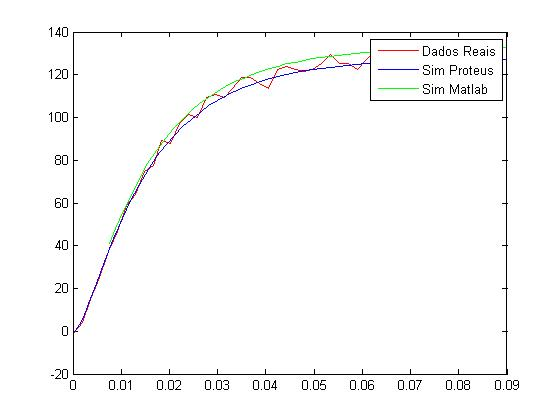
\includegraphics[width=.7\textwidth]{Dados_reais_matlab_proteus_malha_aberta.jpg}
\caption{Dados Reais , Simulação Proteus e Matlab}
\label{dados reais e simulacao}
\end{figure}


\begin{figure}[h!]
\centering
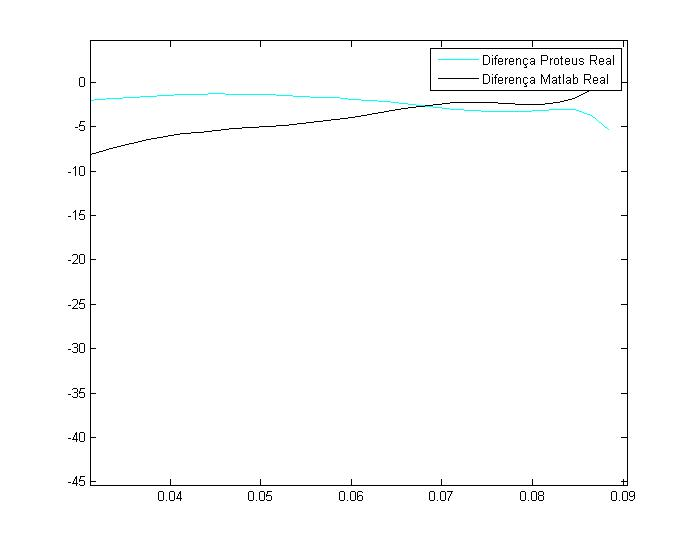
\includegraphics[width=.7\textwidth]{erro_malha_aberta.jpg}
\caption{Erro Com Relação aos Dados Reais da Simulação no Proteus e Matlab em Malha Aberta}
\label{erro Malhaaberta}
\end{figure}

Assim, verifica-se que ambas as simulações obtiveram erros razoáveis com os dados obitidos experimentalmente.Porém, cabe salientar que foi usado no proteus 
os blocos de função de transferência, que não é seu ponto forte, afinal não há uma grande gama de funções.No que diz respeito a simulação do controle do motor 
em malha fechada, caberá o uso de componentes reais do Proteus, sendo este seu ponto forte.Isto é conteúdo dos próximos tópicos.

\newpage

\section{Simulações do Controle em Malha Fechada.}
A simulação foi realizada no software Proteus utilizando os componentes e resistências que compõem o controlador, utilizando blocos para representar o PWM e 
o ganho do tacogerador, além da planta do motor.A figura (\ref{Circ_proteus}) ilustra a construção feita.

\begin{figure}[h!]
\centering
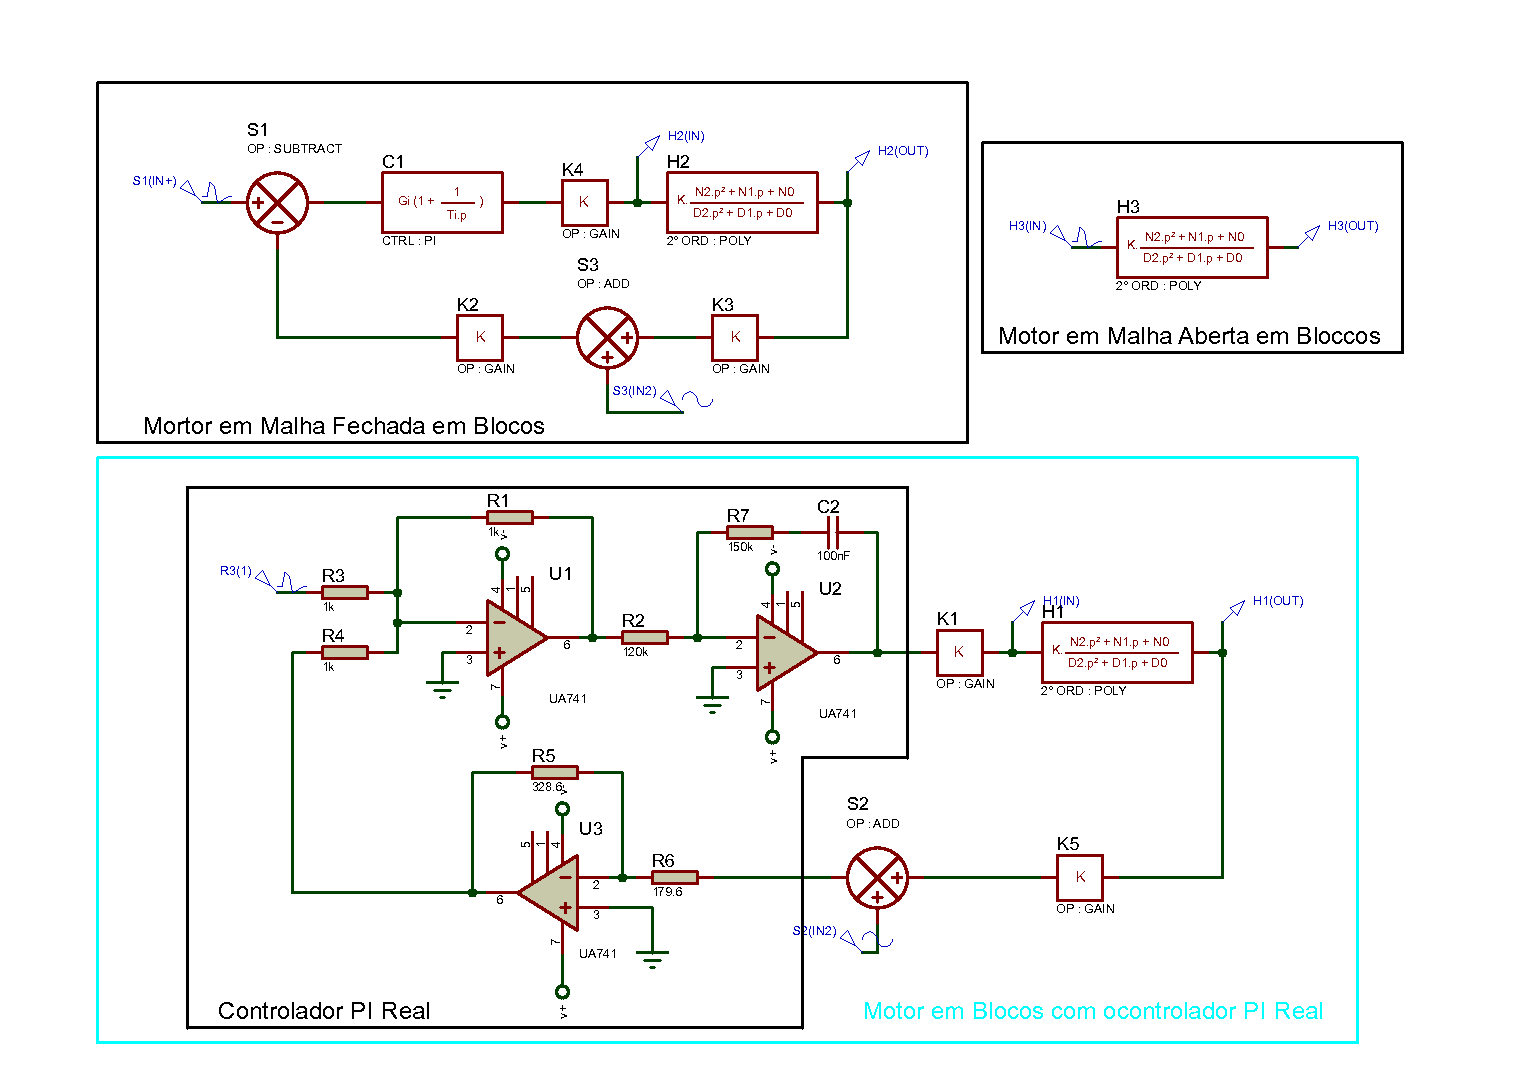
\includegraphics[width=.9\textwidth]{circuito_proteus.pdf}
\caption{Estrutura Simulada no Proteus com os Componentes Reais do Controlador}
\label{Circ_proteus}
\end{figure}

Foram feitas as simulações nos softwares Matlab e Proteus e plotadas juntamente com o intuito de verificar a precisão das simulações nos softwares, 
principalmente no proteus, por ser de menor reputação.A resposta real também foi plotada para verificar a precisão.Tal construção de simulações encontra-se 
na figura abaixo (\ref{sim_pro_mat}).


\begin{figure}[h!]
\centering
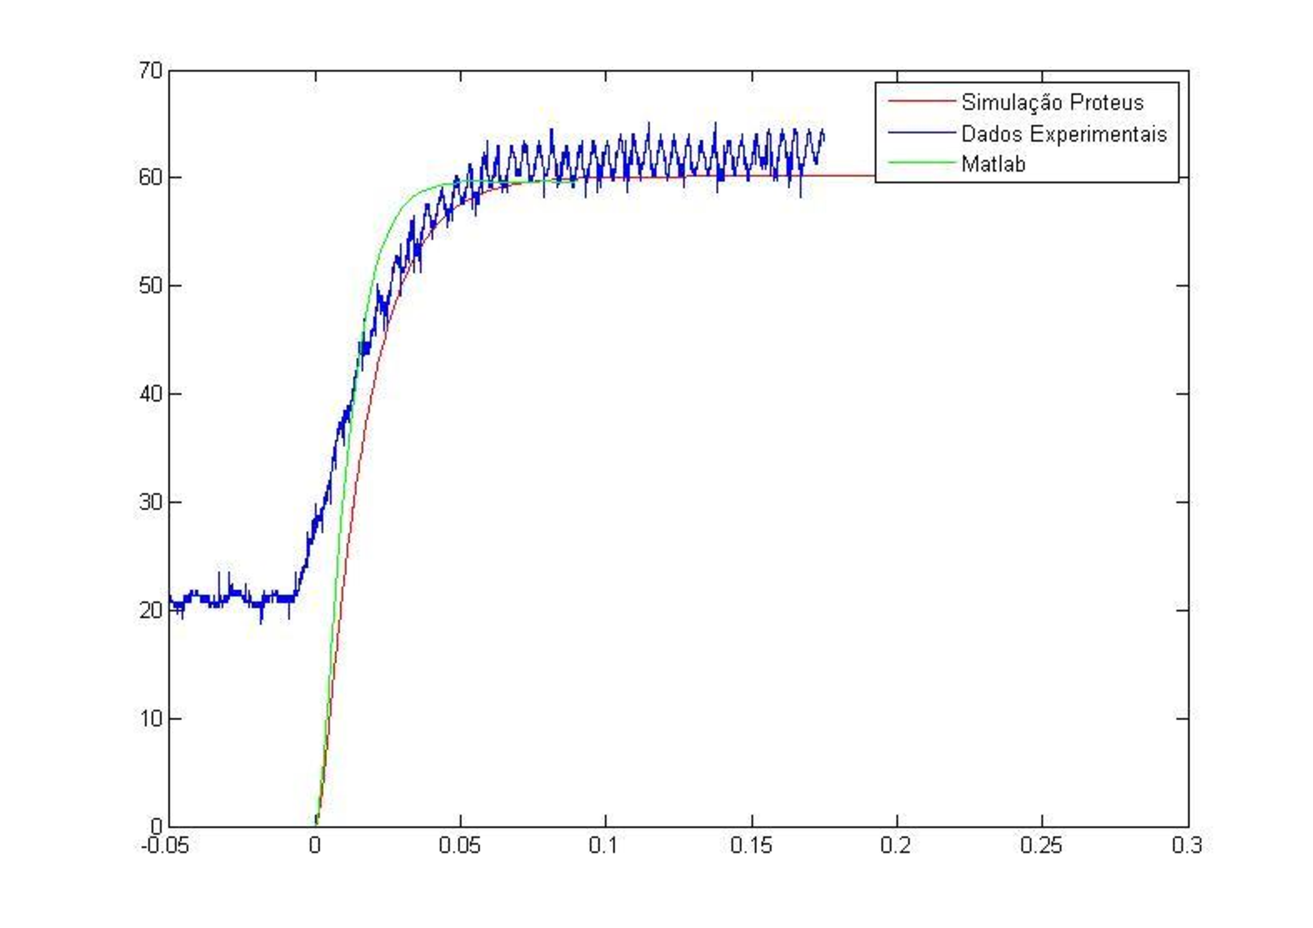
\includegraphics[width=.7\textwidth]{Comparacao_mat_pro_real_m_fechada.pdf}
\caption{Estrutura Simulada no Proteus e Matlab e Dados Obtidos Experimentalmente}
\label{sim_pro_mat}
\end{figure}

Por meio das comparações feitas entre os simuladores e dados obtidos no laboratório, verifica-se que são confiáveis as simulações no proteus para blocos de 
controle e amp-ops.

\section{Simulação PWM no Proteus e Construção da Placa de Controle}
O PWM é uma construção essencial no controle do motor, e  seu funcionamento, no quesito de componentes analógicos, se da por meio da comparação da forma de 
onda de uma dente de serra com uma tensão de referência.Conforme varia-se a tensão de referência  varia-se o duty cycle do PWM.A figura (\ref{PWM}) explicita
o circuito do PWM utilizado, sendo que a figura (\ref{Simulacao_PWM_Proteus1}) expressa a simulação do componente.A simulação foi realizada com uma tensão de 
entrada no valor de  5,96 Volts, gerando o duty cycle precisamente como mostra a tabela (\ref{Simulacao_PWM_Proteus1}) que é de valor 52us.

\begin{figure}[h!]
\centering
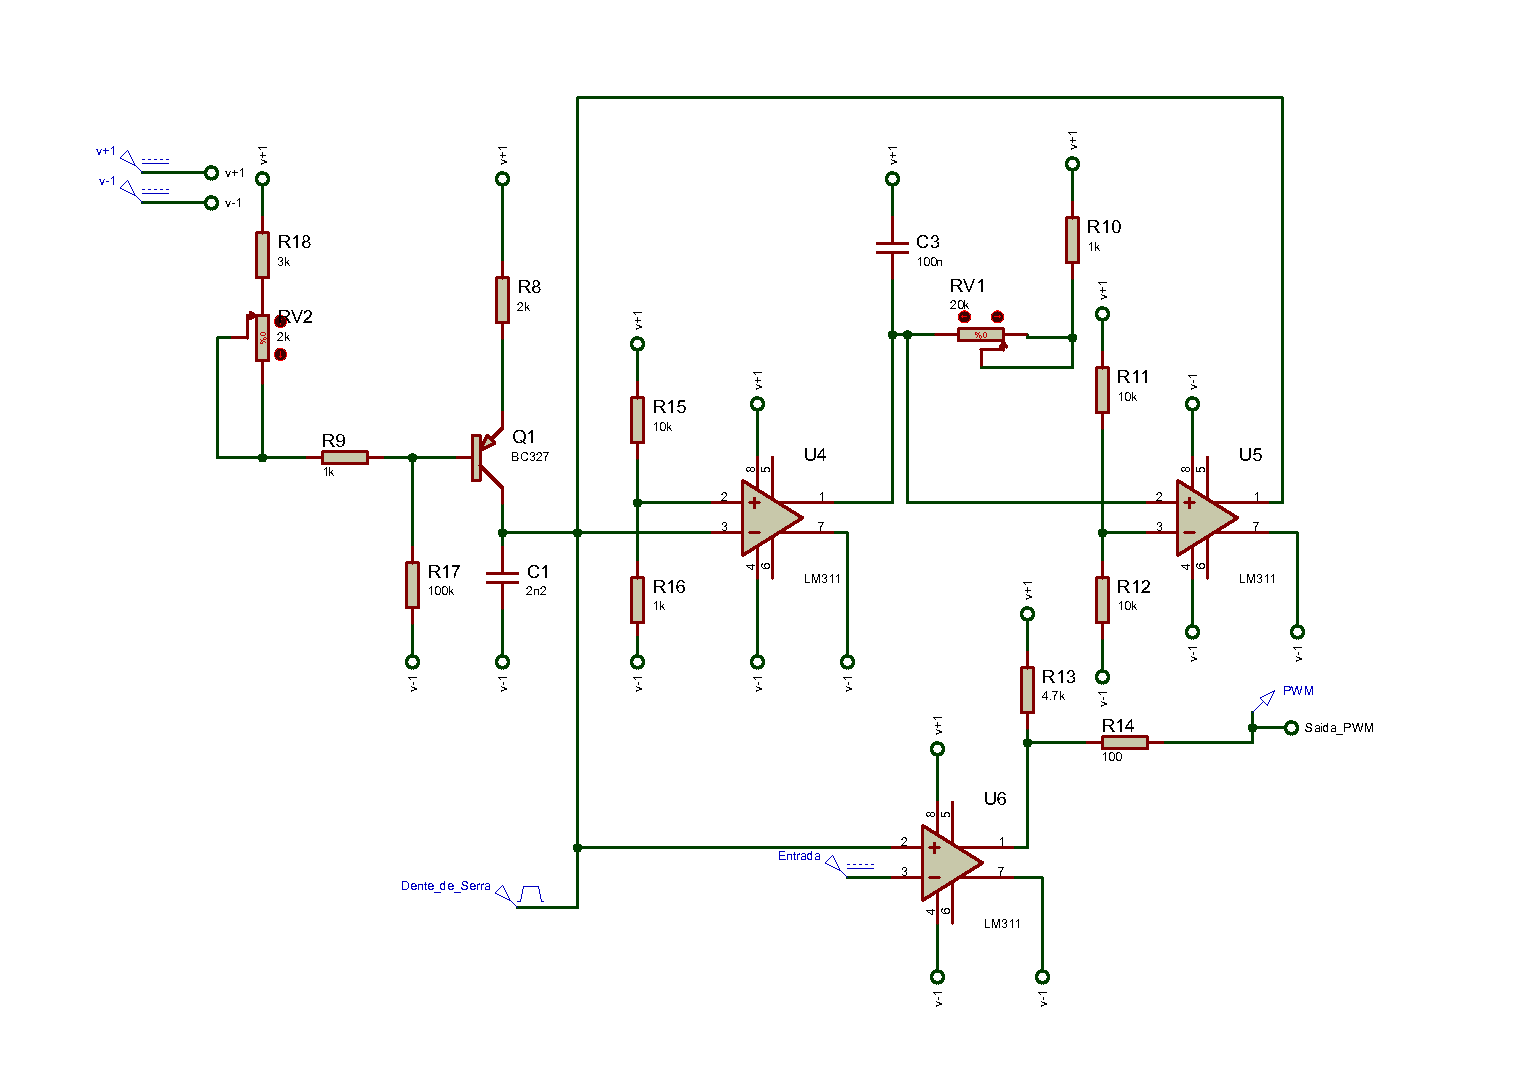
\includegraphics[width=.9\textwidth]{pwm.pdf}
\caption{Circuito PWM}
\label{PWM}
\end{figure}

\begin{figure}[h!]
\centering
\includegraphics[width=.5\textwidth]{simulacao_pwm_proteus.pdf}
\caption{Simulação do Circuito PWM da Figura Acima.}
\label{Simulacao_PWM_Proteus1}
\end{figure}

Como foi dito, o software Proteus possibilita a construção da placa de controle, além de sua simulação.Assim, a construção do projeto se dá quando todas as 
simulações estarem batendo com os resultados esperados, expresando essa vantagem como explicito na figura (\ref{PCB_esquematico}).O circuito em sua forma de 
simulação e renderização para o circuito real encontram-se nas figuras (\ref{PCB}), (\ref{Real}) abaixo.Com esta placa o controle do motor pode ser feito 
apenas conectando os elementos expressos na figura da placa real renderizada, sendo que  TC é a saida do Tacogerador, $+15V$ o 15 volts e $-15V$ o  menos 
15 volts, $D_S$ a entrada dente de serra, se não se desejar colocar um componente que gere tal forma de onda na placa como o LM555 que é um dos CI's capaz 
de gerar essa forma  de onda, IN é tensão de referência para o PWMS e a saída do PWM que vai para o terminal do motor.

\begin{figure}[h!]
\centering
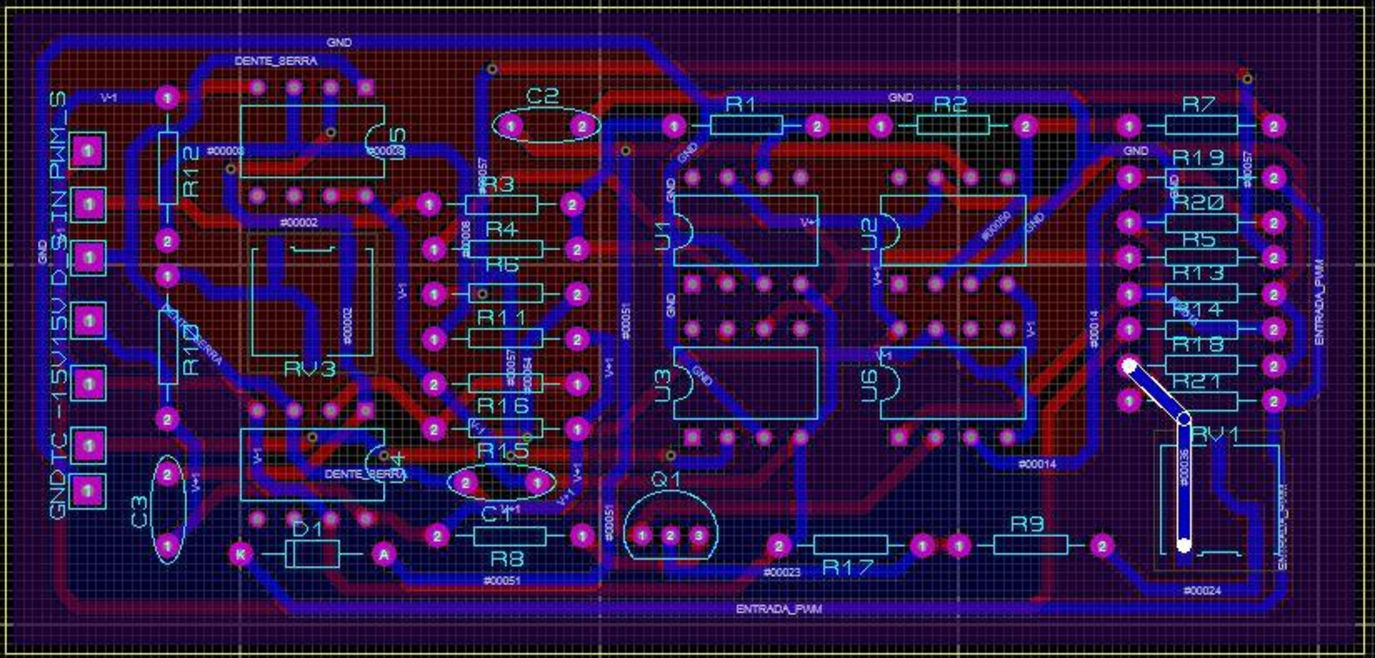
\includegraphics[width=.5\textwidth]{Proteus_PCB.pdf}
\caption{Imagem na Forma de PCB Construida no Software Proteus Ares}
\label{PCB}
\end{figure}

\begin{figure}[h!]
\centering
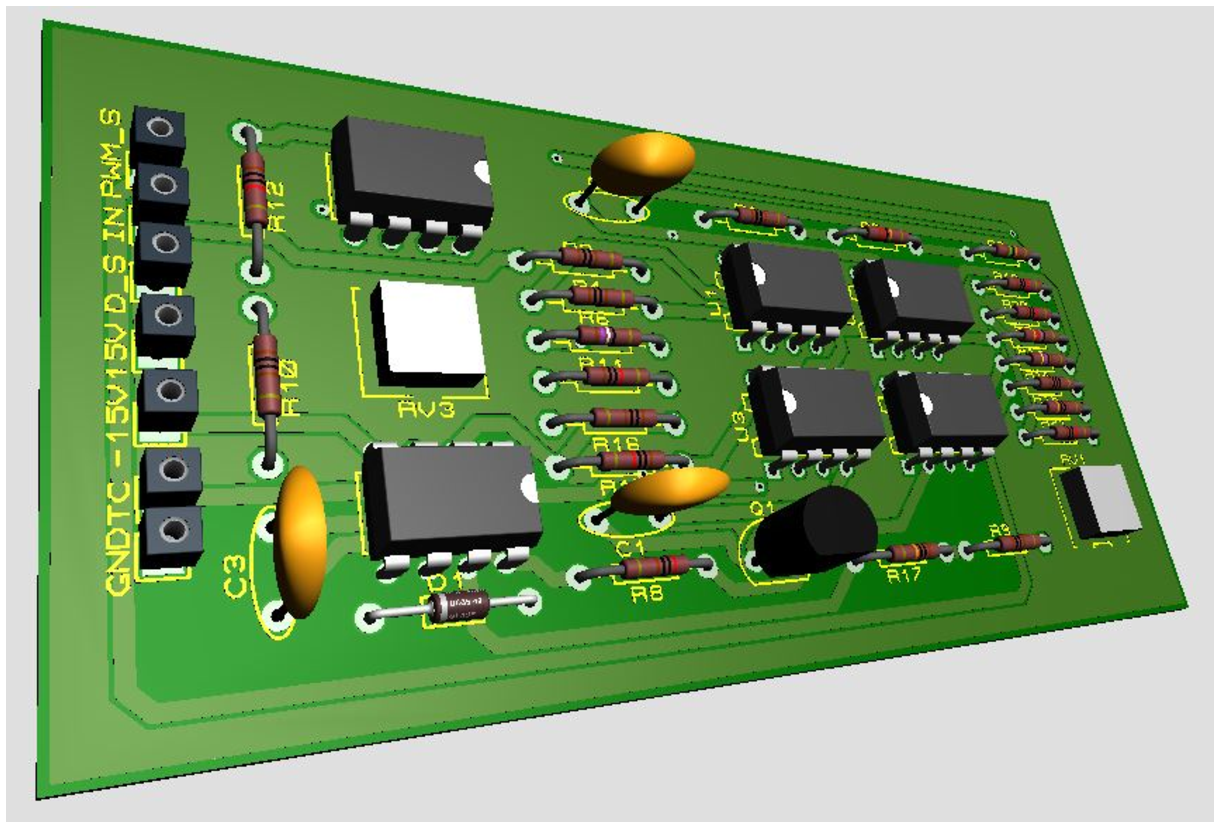
\includegraphics[width=.5\textwidth]{Proteus_Real.pdf}
\caption{Placa Renderizada do Circuito PCB Acima.}
\label{Real}
\end{figure}

\newpage

\section{Conclusão Simulação Proteus}
Como pode ser visto pela comparação das simulações, observa-se que o proteus possui grande fidelidade quanto a simulações, 
havendo pequena diferença entre a simulação no matlab, dados reais.O fato de poder-se simular e construir o circuito simulado 
é uma grande vantagem, afinal garante-se que o sistema terá o funcionamento desejado.Assim, conclui-se que tal software é um bom 
simulador para auxiliar em projetos de controle.



\newpage

\bibliography{80c51} 
\bibliographystyle{ieeetr}



\end{document} 

